\documentclass[11pt,a4paper]{report}

% --- Mandatory layout constraints (HAN) ---
\usepackage[a4paper,margin=2.5cm]{geometry} % >= 2.5cm margins :contentReference[oaicite:4]{index=4}
\usepackage{setspace}
\setstretch{1.2} % >= 1.2 line spacing :contentReference[oaicite:5]{index=5}

% ---------- Fancy headers (Report) ----------
\usepackage{xcolor}
\usepackage{fancyhdr}
\setlength{\headheight}{24pt}
\addtolength{\topmargin}{-12pt}

\pagestyle{fancy}
\fancyhf{}

% Put chapter title in left header
\renewcommand{\chaptermark}[1]{\markboth{#1}{}}
\fancyhead[L]{\nouppercase{\leftmark}}

% Right header text
\fancyhead[R]{Project Report}

% Page number
\fancyfoot[C]{\thepage}

\renewcommand{\headrulewidth}{0.4pt}
\renewcommand{\footrulewidth}{0pt}

% Red header rule
\makeatletter
\renewcommand{\headrule}{%
  {\color{blue}\hrule width\headwidth height\headrulewidth \vskip-\headrulewidth}%
}
\makeatother

% Apply same header style on chapter-opening pages (plain style)
\fancypagestyle{plain}{%
  \fancyhf{}
  \fancyhead[L]{\nouppercase{\leftmark}}
  \fancyhead[R]{Project Report}
  \fancyfoot[C]{\thepage}
  \renewcommand{\headrulewidth}{0.4pt}
  \renewcommand{\footrulewidth}{0pt}
  \makeatletter
  \renewcommand{\headrule}{%
    {\color{blue}\hrule width\headwidth height\headrulewidth \vskip-\headrulewidth}%
  }
  \makeatother
}
% -------------------------------------------

% --- Common packages ---


\usepackage{graphicx}
\usepackage{float}
\usepackage{amsmath,amssymb}
\usepackage{array}
\usepackage{booktabs}
\usepackage{longtable}
\usepackage{url}
\usepackage[square,numbers]{natbib}
\usepackage[hidelinks]{hyperref}

\usepackage[acronym,nomain,nonumberlist,toc]{glossaries}
\makenoidxglossaries
\newacronym{ai}{AI}{Artificial Intelligence}
\newacronym{adc}{ADC}{Active Data Collector}
\newacronym{apa}{APA}{American Psychological Association}
\newacronym{ap}{AP}{Average Precision}
\newacronym{cnn}{CNN}{Convolutional Neural Network}
\newacronym{coco}{COCO}{Common Objects in Context}
\newacronym{cpu}{CPU}{Central Processing Unit}
\newacronym{cv}{CV}{Computer Vision}
\newacronym{cvat}{CVAT}{Computer Vision Annotation Tool}
\newacronym{cuda}{CUDA}{Compute Unified Device Architecture}
\newacronym{dl}{DL}{Deep Learning}
\newacronym{fp16}{FP16}{Half-precision floating point format}
\newacronym{fps}{FPS}{Frames Per Second}
\newacronym{gpu}{GPU}{Graphics Processing Unit}
\newacronym{ieee}{IEEE}{Institute of Electrical and Electronics Engineers}
\newacronym{iou}{IoU}{Intersection over Union}
\newacronym{json}{JSON}{JavaScript Object Notation}
\newacronym{jetson}{NVIDIA Jetson}{Embedded GPU platform for edge AI}
\newacronym{map}{mAP}{Mean Average Precision}
\newacronym{ml}{ML}{Machine Learning}
\newacronym{ocr}{OCR}{Optical Character Recognition}
\newacronym{onnx}{ONNX}{Open Neural Network Exchange}
\newacronym{paddleocr}{PaddleOCR}{Paddle Optical Character Recognition}
\newacronym{rgb}{RGB}{Red--Green--Blue}
\newacronym{rgbd}{RGB-D}{Red--Green--Blue plus Depth}
\newacronym{rnn}{RNN}{Recurrent Neural Network}
\newacronym{ros}{ROS}{Robot Operating System}
\newacronym{ros2}{ROS 2}{Robot Operating System 2}
\newacronym{slam}{SLAM}{Simultaneous Localization and Mapping}
\newacronym{sota}{SOTA}{State of the Art}
\newacronym{tensorrt}{TensorRT}{TensorRT}
\newacronym{tbd}{TBD}{To Be Determined}
\newacronym{wsl}{WSL2}{Windows Subsystem for Linux 2}
\newacronym{wandb}{W\&B}{Weights \& Biases}
\newacronym{vram}{VRAM}{Video Random Access Memory}
\newacronym{xml}{XML}{Extensible Markup Language}
\newacronym{yaml}{YAML}{YAML Ain't Markup Language}
\newacronym{yolo}{YOLO}{You Only Look Once}
\newacronym{maskrcnn}{Mask R-CNN}{Mask Region-Based Convolutional Neural Network}

\setglossarystyle{long}
\renewcommand*{\glsgroupskip}{}
\setlength{\glsdescwidth}{0.78\textwidth}


\usepackage{wrapfig}
\usepackage{caption}
\usepackage{titlesec}
\AtEndDocument{\makeatletter}
% Make chapters look like: "1 Introduction" (no "CHAPTER 1")
\titleformat{\chapter}[hang]
  {\normalfont\Large\bfseries}
  {\thechapter\quad}
  {0pt}
  {}
\titlespacing*{\chapter}{0pt}{0pt}{1em}


% --- Bibliography (BibTeX) ---
\bibliographystyle{apalike}

\begin{document}

% ---------- Front matter (roman numbering) ----------
\pagenumbering{roman}

% Title page (adjust to match the template’s first pages)
\begin{titlepage}
    \centering
    \vspace*{2cm}
    {\Large Master Engineering Systems\par}
    \vspace{1cm}
    {\LARGE\bfseries Major Project Report\par}
    \vspace{1.5cm}
    {\huge\bfseries Developing a Scalable Computer-Vision Pipeline for\\
    Human--Interaction Element Detection in Hospital Environments\par}
    \vspace{2cm}
    {\Large Pavel Petrovski\par}
    \vspace{0.5cm}
    {\large HAN University of Applied Sciences\par}
    \vfill
    {\large Supervisors: Siddharth Ajaykumar, Jan Benders, Ben Pyman\par}
    \vspace{0.5cm}
    {\large \today\par}

    \begin{center}
    
\includegraphics[width=6cm]{figures/HANlogo.png}

    \vspace{0.5cm}
    \textbf{Master Engineering Systems – Major Project}\\
    Cyber-Physical Systems\\
    HAN University of Applied Sciences\\
    Arnhem
\end{center}
\end{titlepage}

% Preface / Disclaimer / Summary (as in template)
\chapter*{Preface}
\addcontentsline{toc}{chapter}{Preface}

This report presents the work carried out as part of the Master thesis project in
Cyber-Physical Systems track of the Master Engineering Systems program at HAN University of Applied Sciences. The project was conducted
in collaboration with Ambyon and HAN Automotive Research.

The objective of the thesis is to design and evaluate a scalable computer-vision
pipeline for service-robot interaction-point perception in hospital
environments. All work described in this report was performed by the author.

The project repository is available at
\href{https://gitlab.com/han-automotive-research/carebots/master_thesis_carebot_2025}{GitLab},
and experiment tracking together with fine-tuning curves is available at
\href{https://wandb.ai/pavelpetrovski333-han-university-of-applied-sciences/projects}{Weights \& Biases}.


\chapter*{Disclaimer}
\addcontentsline{toc}{chapter}{Disclaimer}
This Project Report was written independently by the author as part of the Master of Engineering Systems program at HAN University of Applied Sciences.  

During the preparation of this report, the generative artificial intelligence tool
\textit{ChatGPT} (OpenAI, 2025) was used selectively to support the writing process.
The tool was employed to assist with improving sentence structure, refining academic
language, and suggesting minor text rephrasing.

All technical content, system design decisions, experimental implementation,
training procedures, evaluation methods, and results presented in this report are
the original work of the author. The use of the AI tool did not replace independent
analysis, interpretation of scientific literature, or critical reasoning.


The use of AI complies with the \textit{MES Policy on the Use of Generative AI}, ensuring informed, transparent, ethical, and responsible application.


\chapter*{Summary}
\addcontentsline{toc}{chapter}{Summary}
This report presents work carried out within the CareBot projects at HAN
University of Applied Sciences in collaboration with
\href{https://ambyon.care}{Ambyon}. The project addresses the need for reliable
robot perception of elevator buttons in hospital environments, where autonomous
navigation across floors depends on accurate detection, interpretation, and
spatial localization of panel interfaces.

The developed workflow combines instance segmentation for button localization,
semi-automatic annotation with iterative retraining, and a lightweight optical
character recognition model for semantic button interpretation. The original
elevator-panel dataset was extended with instance-level annotations and later
augmented with deployment-specific images from the target university
environment. Detector and recognizer models were trained, tuned, and evaluated
using held-out test data and deployment-oriented runtime benchmarks.

The results show that the final system can combine button segmentation, text
recognition, and depth-based target estimation in a modular embedded perception
pipeline running on NVIDIA Jetson hardware. The project therefore delivers a
practical foundation for elevator-button interaction on the CareBot platform and
for future model improvement through deployment-time data collection and
retraining.


\chapter*{Nomenclature}
\addcontentsline{toc}{chapter}{Nomenclature}

\section*{List of Symbols}
\addcontentsline{toc}{section}{List of Symbols}
\noindent
\begin{tabular}{@{}p{0.22\textwidth}p{0.72\textwidth}@{}}
$\mathcal{L}$ & composite training loss \\
$\lambda$ & weighting coefficient for YOLO loss terms \\
$TP$, $FP$, $FN$ & true positives, false positives, and false negatives \\
$N$ & number of samples \\
$\hat{y}_i$, $y_i$ & predicted and ground-truth OCR labels for sample $i$ \\
$\mathcal{V}$ & set of valid depth pixels inside the predicted segmentation mask \\
$u$, $v$ & image coordinates of the target center \\
$x$, $y$, $z$ & estimated 3D target coordinates \\
$f_x$, $f_y$ & camera focal lengths in pixels \\
$c_x$, $c_y$ & camera principal-point coordinates \\
\end{tabular}

\section*{Acronyms}
\addcontentsline{toc}{section}{Acronyms}
\glsaddall[types=\acronymtype]
{\renewcommand*{\glossarysection}[2][]{%
}%
\printnoidxglossary[
  type=\acronymtype,
  title={}
]}
\clearpage



\tableofcontents
\clearpage

\listoffigures
\clearpage

\listoftables
\clearpage



% ---------- Main matter (arabic numbering) ----------
\pagenumbering{arabic}

% Mandatory chapter structure (do not rename/remove) :contentReference[oaicite:7]{index=7}

\chapter{Introduction}

This introduction includes the background information, problem definition, project objective and the
research questions.

\section{Background}

Robotics in healthcare is moving from experimental pilots to practical deployment, supporting tasks such as logistics, delivery of medical supplies, and environmental assistance. These systems are intended not to replace clinical staff, but to support them by reducing repetitive physical work and enabling more time for patient care \citep{holland2021servicerobots,masala2025assistiverobotics}. As hospitals face increasing operational pressure and staff shortages, autonomous robots capable of safe navigation and interaction with the environment hold significant potential.

\begin{wrapfigure}{r}{0.36\textwidth}
    \centering
    \vspace{-8pt}
    \captionsetup{width=0.34\textwidth}
    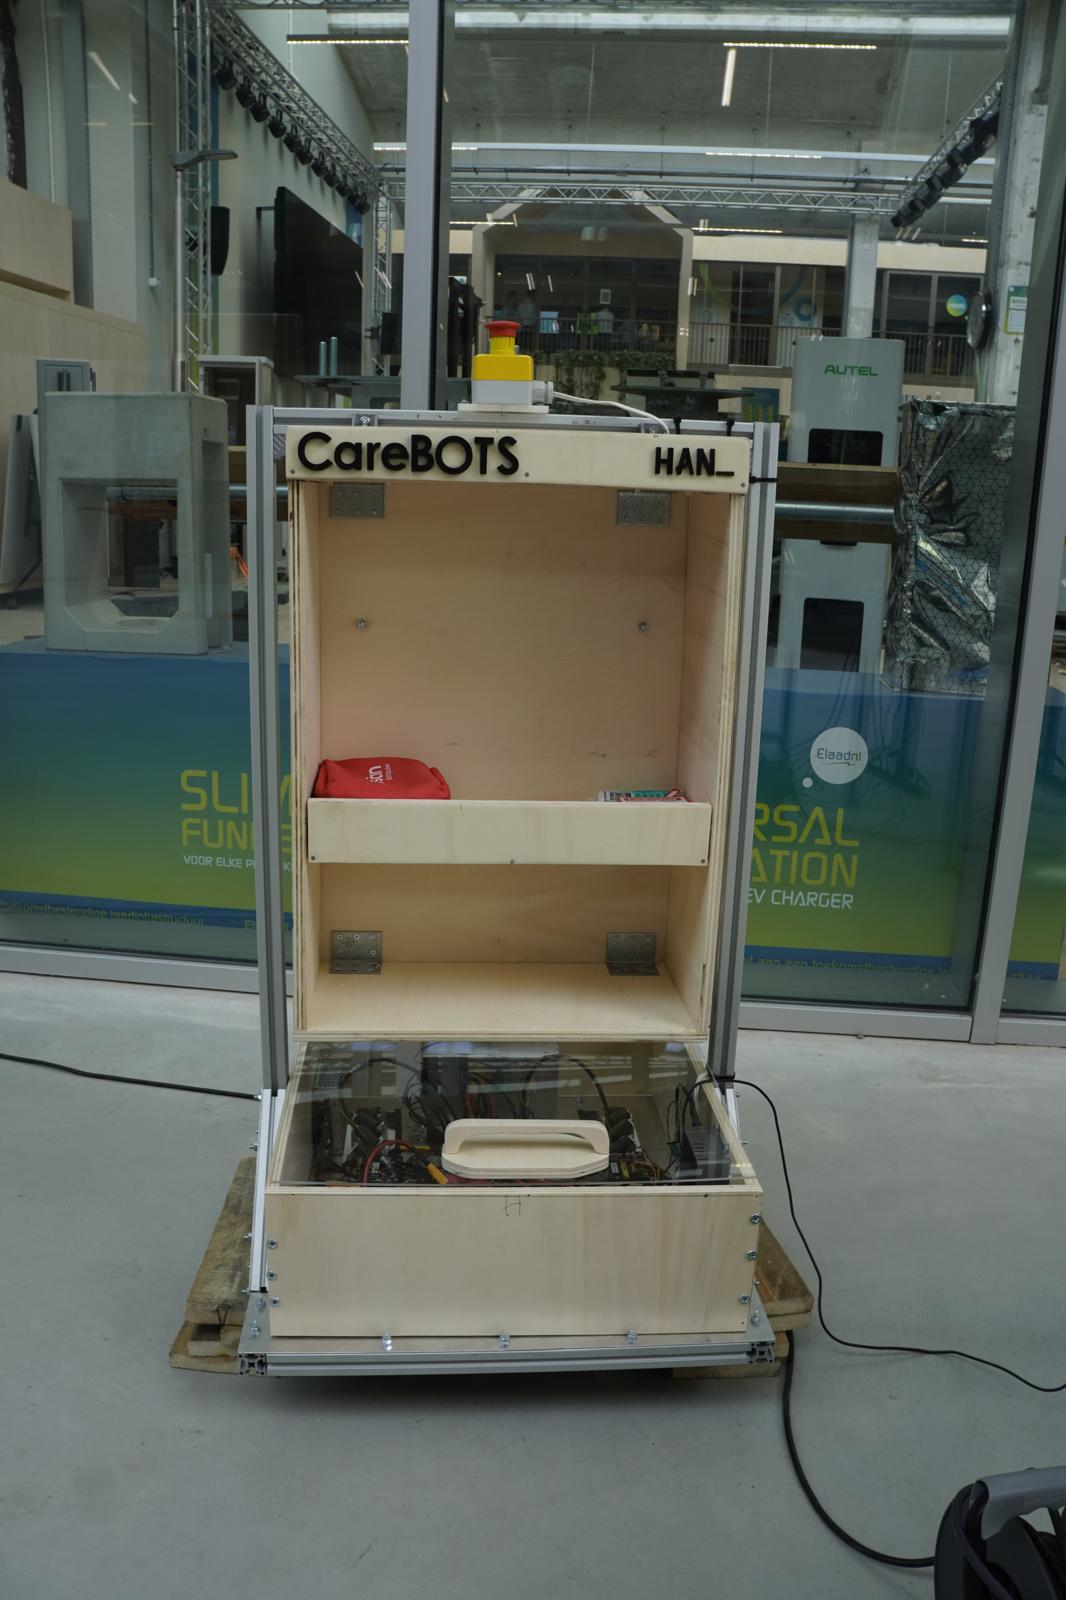
\includegraphics[width=0.45\textwidth]{figures/carebot.jpg}
    \caption{CareBot prototype at HAN Automotive Research}
    \label{fig:prototyperobot}
    \vspace{-8pt}
\end{wrapfigure}

Hospitals are typically multi-floor environments that rely on infrastructure such as elevators, automatic doors, and access-control systems. For a robot to move freely and perform tasks across different floors, it must be able to detect and interact with these human–machine interfaces, including elevator buttons and door panels. Reliable perception of such interaction elements is therefore a key capability for achieving truly autonomous navigation in hospital settings. Without this, robots remain confined to limited single-floor operation or require human assistance for vertical transport.

At \textit{HAN Automotive Research}, the CareBot platform is being developed as an educational and research project that allows students and researchers to experiment with robotic perception, planning, and control in realistic environments. While not designed to replicate the Ambyon ONE robot, the CareBot in this project will be equipped with a similar sensor stack and processing unit, enabling realistic simulation of Ambyon’s operational conditions. The Ambyon ONE itself is a service robot currently under development by \textit{Ambyon}, a Dutch startup focused on robotics for healthcare and logistics applications.

The CareBot system uses an \gls{rgbd} camera and \gls{jetson} computing module to enable on-device perception suitable for real-time operation in clinical environments. A key research challenge is enabling the robot to accurately detect and classify interaction points such as elevator buttons, access readers, and door panels under varying lighting, reflections, occlusions, and diverse panel designs - while maintaining efficient performance within embedded hardware constraints.

This project contributes to that research direction by designing and evaluating a scalable computer-vision workflow for interaction-point detection on embedded systems. The work includes dataset creation, model design and optimisation, evaluation on prototype hardware, and preparation for future extensions. The resulting system will serve as a foundation for autonomous hospital mobility and support the development of assistive robotic technologies.

%---------------------------------------------------------------

\section{Problem Definition}
% The Ambyon ONE robot currently lacks a robust and efficient perception system capable of reliably detecting and localizing human-interaction elements such as elevator buttons, door panels, and access systems in hospital environments in real time on Jetson-class embedded hardware, under variable conditions and panel layouts.
The Ambyon ONE robot currently lacks a reliable computer-vision system to detect and recognize human-interaction elements (e.g., elevator and door control interfaces) in hospital environments, preventing autonomous navigation and interaction with building infrastructure.

\section{Project Objective}
% Develop and validate an efficient and scalable computer vision workflow that enables the Ambyon ONE robot to autonomously detect and classify human-interaction elements in hospital environments using embedded hardware.
Develop and validate an efficient and scalable computer-vision workflow that enables a service-robot platform to autonomously detect and classify human-interaction elements in hospital environments using embedded hardware.

\section{Research Question(s)}
\textbf{Main Research Question:} \\
How can an efficient and scalable computer-vision workflow be designed and implemented to enable a service robot to detect and interpret human-interaction elements in hospital environments using embedded hardware?

\textbf{Sub-questions:}
\begin{enumerate}
    \item What are the relevant human–interaction points in hospital environments that should be detected and classified by the computer-vision workflow?
    \item What computer-vision methods and model architectures are most suitable for detecting and classifying human-interaction elements in service-robot environments?
    \item How can a high-quality dataset be designed and constructed for achieving robust model performance?
    \item Which model-optimization techniques support real-time inference on embedded hardware while preserving detection accuracy?
    \item How can the workflow support scalable and efficient model improvements, including potential data collection and retraining during deployment?
\end{enumerate}


\section{Outline of the report}

Chapter~1 introduces the background, motivation, and objectives of the project.
Chapter~2 reviews relevant literature on interaction-point perception, instance
segmentation, and embedded computer-vision systems. Chapter~3 describes the
methodology, including dataset preparation, annotation strategy, model training,
evaluation, and deployment considerations. Chapter~4 presents the experimental
results and quantitative evaluation. Chapter~5 discusses the findings and their
implications, and Chapter~6 concludes the report and outlines future work.


\chapter{Literature Review}
\label{ch:literature}
This chapter reviews the scientific literature relevant to interaction-point
perception in hospital environments, with a focus on instance segmentation,
dataset design, annotation strategies, and deployment of computer-vision models
on embedded systems.

\section{Perception of human-machine interaction elements}

Human--machine interaction elements such as elevator buttons, door panels, and
access readers are important targets for indoor service robots operating in
hospital environments. Previous work in healthcare and service robotics shows
that reliable interaction with such infrastructure is required for autonomous
operation across multiple floors and restricted areas
\citep{holland2021servicerobots,masala2025assistiverobotics}.

From a computer-vision perspective, these interaction elements are challenging
to detect because they are small, visually similar, and often arranged closely
together on control panels. Studies on visual perception for robotic interaction
report that elevator panels typically contain many buttons with minimal visual
differences, which makes robust localization difficult under varying lighting
conditions, reflections, and viewing angles \citep{bernard2020interfaces}.

General indoor-robot perception systems often focus on detecting large objects
or structural elements and assume that interaction with building infrastructure
is externally supported or environment-specific. However, research on autonomous
service robots emphasizes that scalable deployment requires perception systems
that can directly identify actionable interface elements from camera and sensor data,
without relying on prior knowledge of the environment
\citep{wang2019indoorrobots}.

These findings indicate that interaction-point perception is a fine-grained
vision problem in which individual button instances on a panel must be localized
accurately within visually dense scenes. At the same time, the cited studies
mainly motivate the problem rather than solving it under the embedded and
deployment-oriented constraints of this project. This observation motivates the
need for vision methods that go beyond coarse detection of panels or regions and
instead support precise identification of individual button instances.


\section{Formulating interaction-point perception as a vision problem}

Vision-based perception problems in robotics are commonly formulated as image
classification, object detection, or semantic segmentation tasks. Each formulation
implies different assumptions about the structure of the scene and the required
output, which directly affects suitability for robotic interaction.

Image classification assigns a single label to an entire image and is therefore
unsuitable for scenarios where multiple interaction elements appear simultaneously.
Object detection extends this formulation by predicting bounding boxes and class
labels for individual objects; in this project, those objects correspond to
individual button instances on an elevator panel. While detection-based approaches have been widely
used for indoor perception tasks, bounding boxes provide only coarse spatial
localization and do not capture the precise shape of interaction elements
\citep{ren2015fasterrcnn,redmon2016yolo}.

Semantic segmentation addresses this limitation by assigning a class label to
each pixel in the image. Formally, semantic segmentation can be expressed as a
pixel-wise classification function
\[
f_{\theta} : \mathbb{R}^{H \times W \times C} \rightarrow \{1,\dots,K\}^{H \times W},
\]
where $H$ and $W$ denote image height and width, $C$ the number of input channels,
and $K$ the number of semantic classes \citep{long2015fcn}. Although this formulation
enables precise localization, all pixels belonging to the same class are treated
as a single region. As a result, semantic segmentation cannot distinguish between
multiple instances of the same object class.

For interaction-point perception, this limitation is critical. Elevator panels
often contain many visually similar button instances, each corresponding to a
distinct action \citep{bernard2020interfaces}. By definition, semantic
segmentation assigns a class label to each pixel but does not separate
same-class instances \citep{long2015fcn}, whereas instance segmentation
predicts a separate mask for each detected instance \citep{he2017maskrcnn}. For an
elevator panel, a semantic segmentation output would therefore label button
pixels by class without separating adjacent buttons into distinct actionable
targets. This lack of instance-level differentiation makes semantic
segmentation unsuitable for downstream decision-making and physical interaction,
where each button must be treated as a separate actionable element.

Instance segmentation extends semantic segmentation by jointly performing object
detection and pixel-wise classification, producing a separate mask for each object
instance. This formulation can be expressed as a set of instance masks
\[
\mathcal{M} = \{M_1, M_2, \dots, M_N\},
\]
where each $M_i \in \{0,1\}^{H \times W}$ represents a binary mask for one object
instance \citep{he2017maskrcnn}. Instance segmentation therefore enables both
precise spatial localization and differentiation between multiple objects of the
same class.
\begin{figure}[htbp]
    \centering
    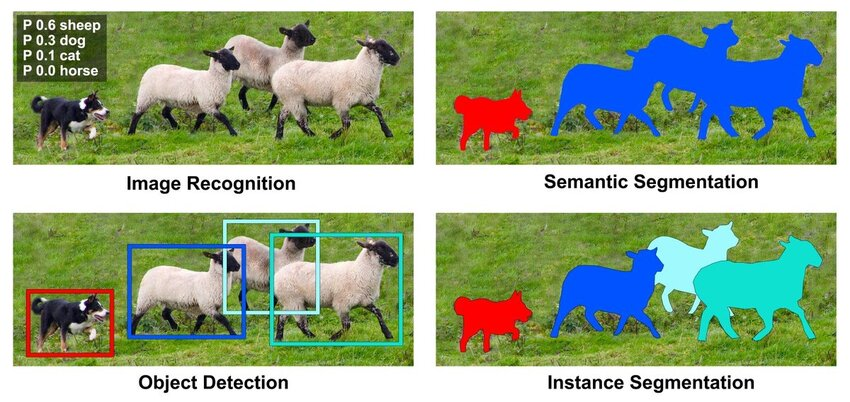
\includegraphics[width=0.9\textwidth]
    {figures/Comparison-of-image-classification-semantic-segmentation-and-semantic-instance.png}
    \caption{Comparison of image classification, object detection, semantic segmentation, and instance segmentation. Adapted from \citet{liu2022indoorscene}.}
    \label{fig:vision_task_comparison}
\end{figure}
Figure~\ref{fig:vision_task_comparison} illustrates the conceptual differences
between image classification, object detection, semantic segmentation, and instance
segmentation for visual perception tasks.


Based on findings in the literature and the requirements of interaction-point
detection, instance segmentation provides the most appropriate problem formulation
for this project. It allows individual buttons to be identified as distinct
entities while preserving pixel-level accuracy, which is essential for reliable
robotic interaction in dense and visually complex control interfaces. The
literature therefore clarifies the correct task formulation, but not yet which
model family best satisfies this requirement on embedded robotic hardware.


\section{Public datasets and annotation strategies.}

Public datasets for vision-based detection of elevator interfaces are limited, as
most indoor robotics datasets focus on navigation or scene understanding rather
than interaction elements \citep{sun2017scenenet}. This limits their direct
applicability to interaction-point perception tasks.

The IRSO 2018 dataset provides \gls{rgb} images of elevator panels captured in realistic
indoor environments and was originally introduced for object detection tasks
\citep{irso2018dataset}. Due to its focus on real elevator interfaces and visual
diversity, it is well suited for studying interaction-point perception in service
robotics.

Recent work reports a large-scale dataset with pixel-wise annotations for elevator
button segmentation \citep{liu2021elevator}. However, despite being described in the
literature, the corresponding semantic segmentation dataset is not publicly
available at the time this project is made and therefore cannot be used.

To enable instance-level interaction-point detection, this work reuses images from
the IRSO 2018 dataset and replaces the original annotations, namely
\gls{xml}-formatted bounding boxes and textual labels, with instance
segmentation masks. The new annotations are stored in the \gls{coco} format,
which supports instance-level labeling and is widely used across computer vision
frameworks, facilitating reuse and future extensions \citep{lin2014coco}. This
reveals a practical gap in the literature: relevant public images exist, but
publicly reusable instance-segmentation annotations for elevator interfaces are
still limited.

\section{Model design principles, evaluation metrics, and semantic interpretation}

Instance segmentation models for robotic perception typically follow a modular
design in which feature extraction, object localization, and pixel-level mask
prediction are handled by separate components within a single network. This design
enables shared visual representations while supporting accurate instance-level
localization, which is required for interaction-point perception in dense control
interfaces.

Region-based instance segmentation models such as \gls{maskrcnn} achieve high
localization accuracy through a two-stage design in which candidate regions are
proposed first and then refined by classification and mask-prediction heads
\citep{he2017maskrcnn}. This architecture is widely used as a reference and
benchmark in instance-segmentation research because of its strong instance-level
accuracy. However, its multi-stage processing increases computational cost and
memory use, which limits suitability for real-time deployment on embedded robotic
platforms.

To address these constraints, single-stage instance-segmentation architectures
have been developed that combine detection and mask prediction in a unified
pipeline. \gls{yolo}-based segmentation models, including the \gls{yolo}v8s
segmentation model, remain CNN-based vision models, but differ from
\gls{maskrcnn} in that they avoid a separate region-proposal stage and are
optimized for faster end-to-end inference \citep{jocher2023yolov8}. In practice,
this design trades some flexibility and, in some cases, peak segmentation
accuracy for substantially improved inference speed and computational efficiency,
which makes such models attractive for embedded robotic deployment.

Model performance is commonly evaluated using overlap-based metrics that measure
agreement between predicted masks and ground-truth annotations. \gls{iou} is defined as
\[
\mathrm{IoU} = \frac{|M_p \cap M_{gt}|}{|M_p \cup M_{gt}|},
\]
where $M_p$ and $M_{gt}$ denote the predicted and ground-truth masks. Average Precision
(\gls{ap}), computed over multiple \gls{iou} thresholds, is widely used as a standard evaluation
metric for instance segmentation tasks \citep{lin2014coco}.

For elevator-button perception, instance localization can be followed by a
recognition stage that determines the functional meaning of each detected button.
This can be achieved using character recognition, \gls{ocr}, or dedicated symbol
classification models applied to isolated button regions \citep{liu2021elevator}.
Accurate instance segmentation is a critical enabling step for such approaches, as
it provides clean, well-aligned inputs for subsequent classification or text
recognition.

In this work, instance segmentation is treated as the primary perception task, as
reliable instance-level localization is a prerequisite for any semantic
interpretation of interaction elements. The resulting pipeline is therefore
designed to support integration of \gls{ocr} or custom button classifiers, enabling the
robot to associate detected buttons with their intended functions in downstream
processing stages. The literature gives clear architectural candidates, but the
trade-off between multi-stage accuracy and single-stage deployability remains an
open design decision for this specific use case.

\section{Embedded deployment constraints in robotic perception}

Vision-based perception systems deployed on mobile service robots must operate
under strict computational and energy constraints. Prior work in robotic vision
reports that deep-learning models deployed on embedded platforms are limited by
onboard memory, processing power, and power consumption, which directly affects
real-time performance \citep{chen2018deeplearningrobots}.

Studies evaluating deep-learning inference on \gls{jetson}-class hardware show that
models achieving high accuracy on desktop \glspl{gpu} often exhibit increased latency and
memory usage when deployed on embedded devices \citep{kang2020edgeai}. These
findings indicate that benchmark accuracy alone is not a sufficient criterion for
model selection in robotic perception systems.

For instance segmentation tasks, this trade-off is particularly relevant, as mask
prediction introduces additional computational overhead compared to bounding-box
detection. Research on efficient model design highlights that architectural choices
such as backbone depth and feature reuse have a significant impact on inference
efficiency \citep{tan2019efficientnet}. Based on these insights, this project
treats model efficiency and deployability as primary design constraints alongside
segmentation accuracy.

Consequently, instance segmentation models considered in this work are evaluated
not only with respect to localization performance, but also in terms of their
suitability for embedded deployment. However, relatively few studies report this
trade-off for elevator-interface perception specifically. This literature-driven
perspective directly informs the model selection and optimization strategies
described in Chapter 3 (\nameref{ch:methodology}).

\section{Scalability, robustness, and reproducibility.}

Several studies emphasize that robust perception systems require more than a single
well-performing model. Instead, scalability is achieved through structured data
management, consistent annotation practices, and reproducible training pipelines
that support incremental dataset expansion and model updates
\citep{cordts2016cityscapes}. These practices reduce sensitivity to domain-specific
bias and enable adaptation to new environments without redesigning the entire
system.

From these findings, this project adopts a pipeline-oriented approach in which
dataset creation, annotation, training, and evaluation are treated as modular and
repeatable processes. Rather than optimizing a single model for a fixed dataset,
the focus is placed on maintaining a perception workflow that can be extended with
new data and retrained as deployment conditions evolve. Existing literature
strongly advocates reproducibility, but gives less attention to practical
feedback loops for environment-specific data collection and retraining after
deployment.


\section{Summary and identified research gap}

The reviewed literature shows that reliable perception of interaction elements in
robotic systems requires instance-level localization, suitable annotation
strategies, and awareness of embedded deployment constraints. Existing studies
demonstrate the technical feasibility of these components, but often address them
in isolation.

At the same time, publicly available datasets for elevator interfaces are limited,
and existing annotations are commonly designed for object detection rather than segmentation tasks. In addition, many approaches focus
on model performance without explicitly considering scalability, reproducibility,
or deployment on embedded robotic platforms.

This project addresses these gaps by repurposing a realistic elevator dataset with
instance-level annotations and by developing a scalable and deployment-aware
computer-vision pipeline for elevator-button perception in hospital environments.
The following chapter describes the methodology used to realize this approach.

\chapter{Methodology}
\label{ch:methodology}

This chapter describes the methodology used to develop a computer-vision pipeline
for interaction-point perception in hospital environments. The project is conducted
with the objective of building a scalable and deployment-oriented perception system
that can be iteratively improved across different hospital settings and reused
within a robot fleet.

\section{Overview of the proposed perception pipeline}

The proposed methodology focuses on instance-level localization of interaction
elements such as elevator buttons and control panels. Instance segmentation is used
to detect individual button instances at pixel level, allowing precise localization
and separation of closely spaced elements. This capability provides the basis for
subsequent interpretation of button functions and autonomous interaction.

The methodology is designed to support an iterative training and deployment
workflow. An initial base model is deployed on the robot, where it performs
interaction-point perception and collects visual data during operation. Selected
data can be transferred to an offboard system, where annotations may be reviewed,
corrected, or extended before retraining the perception models. The updated models
are then redeployed to the robot and become the new default for continued operation.

This workflow enables gradual adaptation to new hospital environments and allows
knowledge acquired in one deployment to be reused and refined in subsequent
deployments. The target end-to-end training and deployment process toward which this
project is developed is illustrated in Figure~\ref{fig:scalable_workflow}.

The following sections describe each stage of the methodology in detail, beginning
with dataset selection and preparation.
\begin{figure}[htbp]
    \centering
    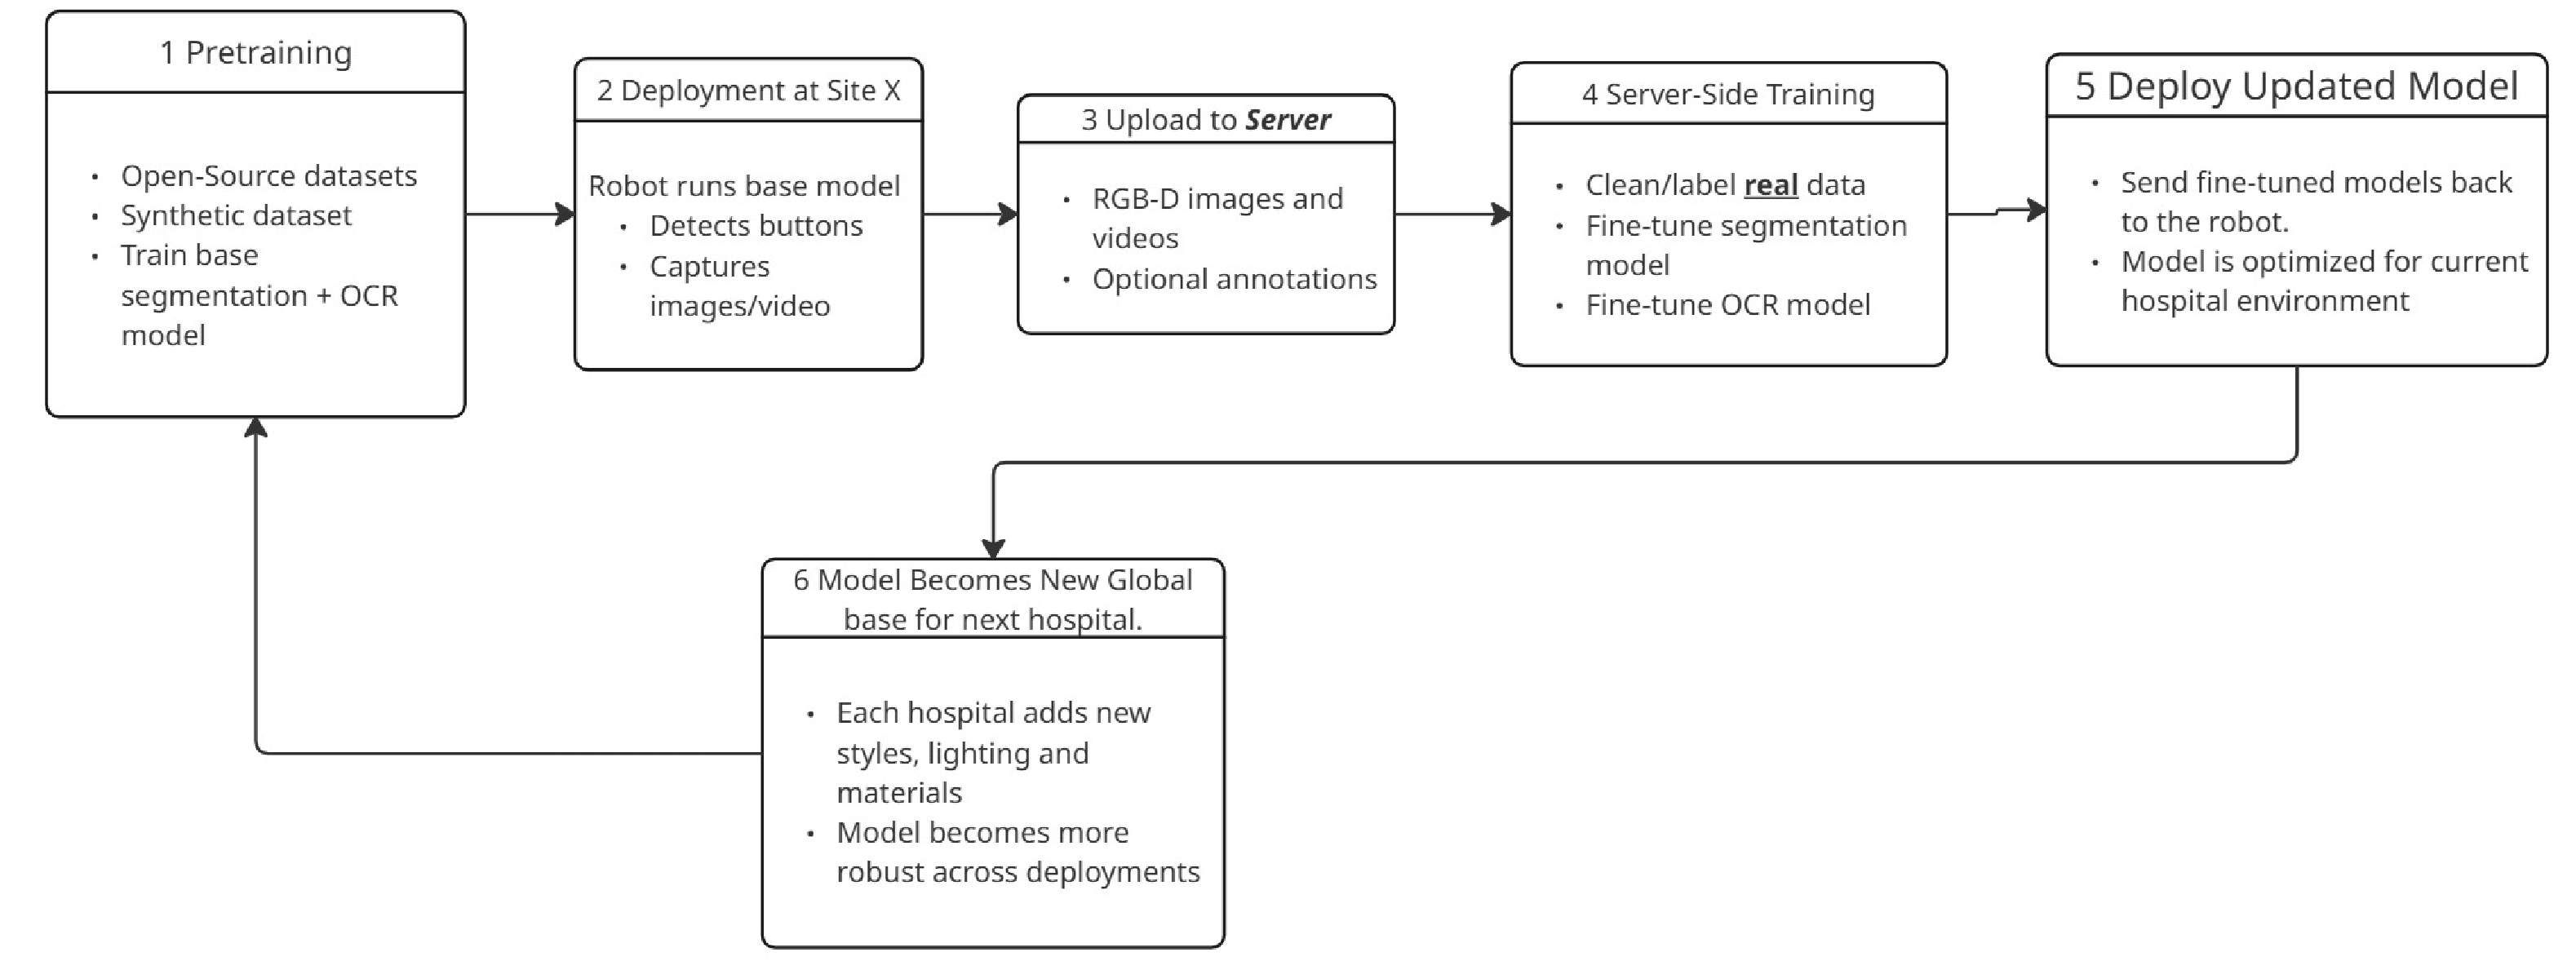
\includegraphics[width=1.1\textwidth]
    {figures/CareBot_workflow.pdf}
    \caption{Target workflow for scalable training and deployment of
    interaction-point perception models across multiple hospital environments.}
    \label{fig:scalable_workflow}
\end{figure}

\section{Dataset selection and preparation}

This project uses a dataset derived from the IRSO2018 collection, which contains
images of elevator panels and buttons captured in realistic indoor environments.
This section corresponds to the initial model-development step in
Figure~\ref{fig:scalable_workflow}, detailing the dataset and its preparation
before the first training cycle.
The origin and relevance of this dataset were discussed in \nameref{ch:literature};
therefore, this section focuses on its structure and preparation for use in this
project.

The dataset consists of a total of 2000 images. Of these, 1400 images are assigned
to the training set (\texttt{train\_set}) and 600 images to the test set
(\texttt{test\_set}). Each subset follows the same directory structure, containing
an \texttt{images} folder with the raw \gls{rgb} images and an \texttt{annotations} folder
with the corresponding annotation files.

In the original dataset, annotations were provided as bounding boxes stored in \gls{xml}
format. For the purposes of this project, the directory structure was preserved,
but the annotation format was replaced with \gls{coco}-style JSON files to support
instance-level segmentation. This ensures compatibility with modern instance
segmentation frameworks while maintaining a clear separation between training and
test data.
\begin{figure}[htbp]
    \centering
    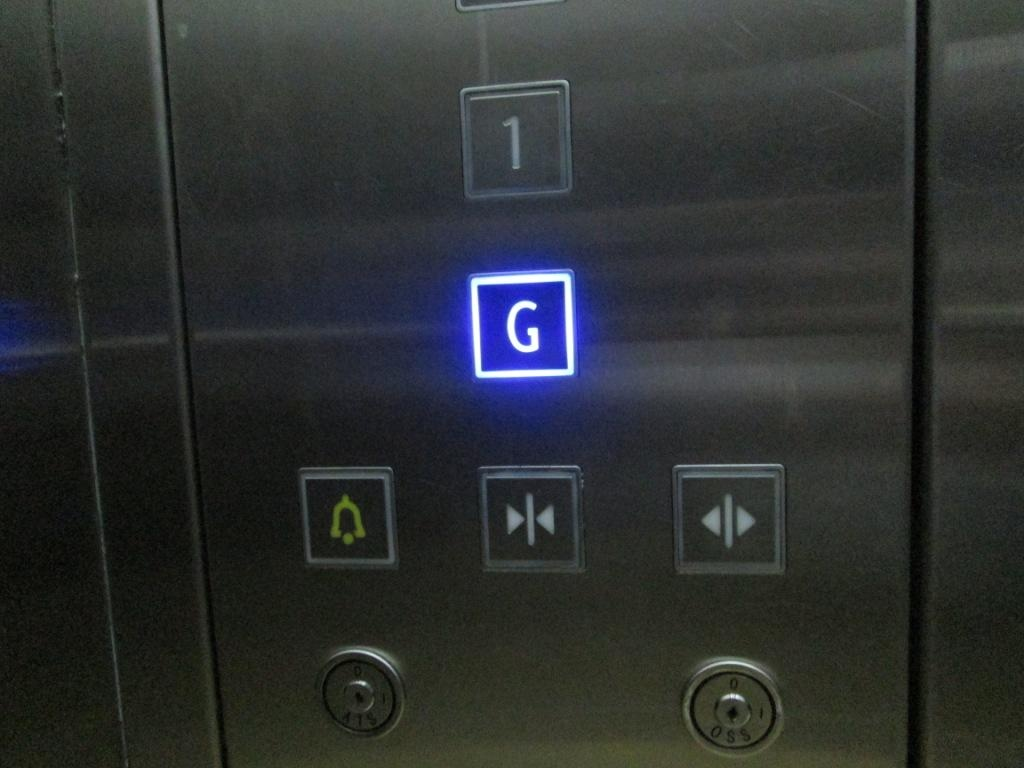
\includegraphics[width=0.4\textwidth]
    {figures/methodology/71.jpg}
    \caption{Example raw image from the dataset.}
    \label{fig:example_raw_image}
\end{figure}

The resulting dataset structure provides a consistent and reusable foundation for
annotation, model training, and evaluation, as described in the following sections.

\section{Annotation strategy and workflow}

Instance-level ground truth was created using a semi-automatic workflow that
combines model-based pre-annotation with manual verification. This strategy was
used to efficiently generate high-quality instance segmentation annotations while
maintaining consistency across the dataset.

Annotations were created in \gls{cvat} \citep{cvat2020}, deployed locally using Docker
\citep{merkel2014docker} within a \gls{wsl}-based Linux environment on a Windows host. Automatic annotation was enabled through \gls{cvat}--Nuclio integration, where the model
was deployed as a Nuclio serverless function \citep{nuclio}. The instance
segmentation model used for automatic annotation was \gls{maskrcnn} \citep{he2017maskrcnn}.

During automatic annotation, \gls{cvat} sends task images to the Nuclio function, where
\gls{maskrcnn} predicts binary masks for each detected button instance. These masks
are converted into polygon shapes within the Nuclio function and returned to \gls{cvat}
as annotation data. The overall workflow used in this project is shown in
Figure~\ref{fig:annotation_workflow}.

\begin{figure}[htbp]
    \centering
    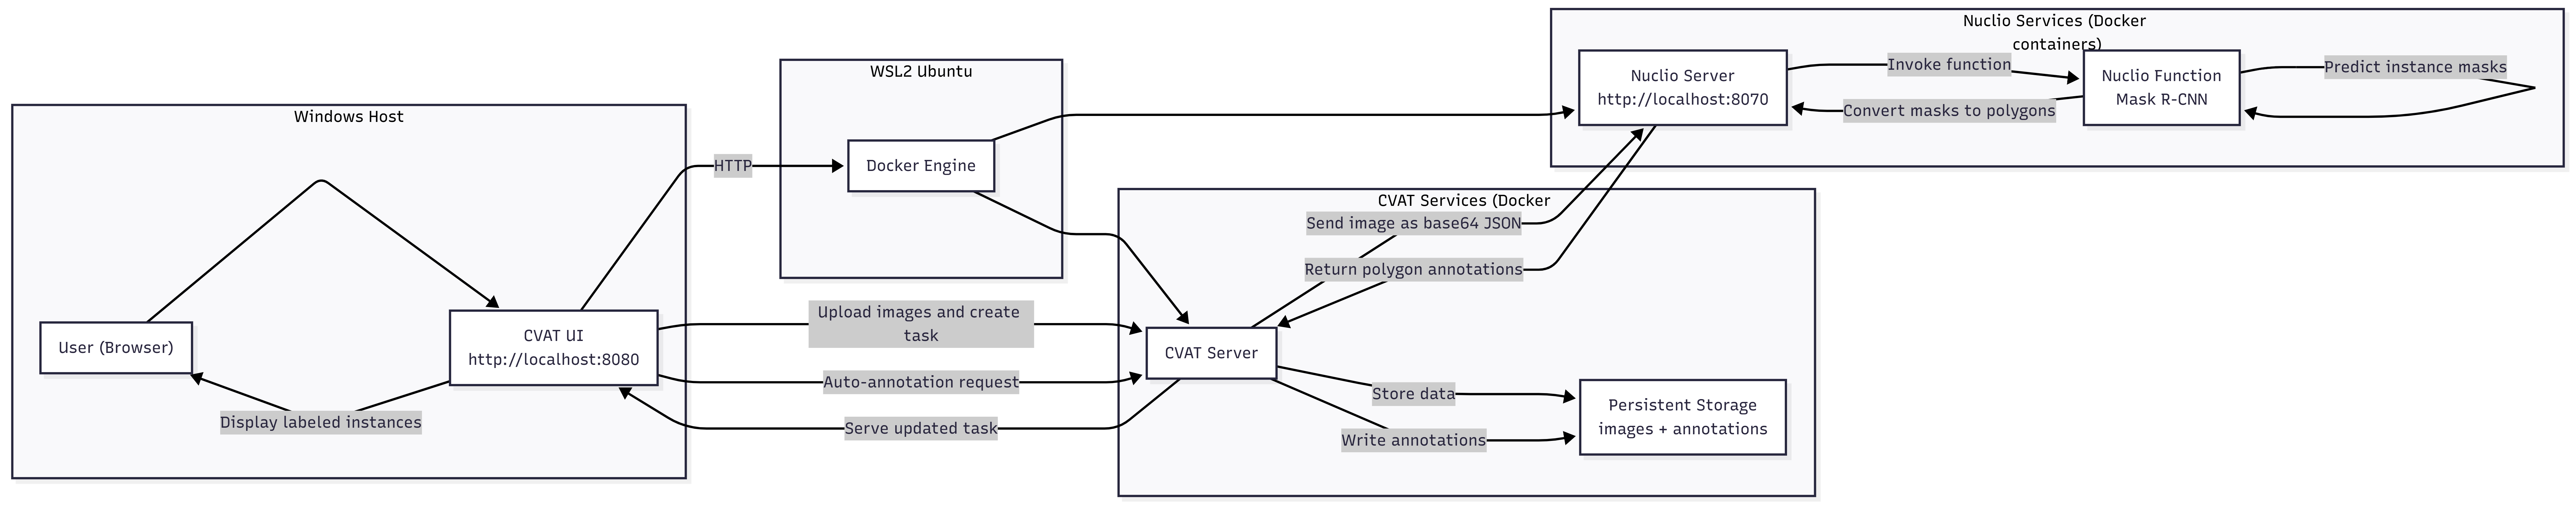
\includegraphics[width=1.3\textwidth]{figures/methodology/Docker_CVAT_Nuclio.png}
    \caption{Semi-automatic annotation workflow on a Windows host using \gls{wsl} and
    Docker. \gls{cvat} sends images to a Nuclio function running \gls{maskrcnn}, which returns
    polygon instance annotations derived from predicted binary masks.}
    \label{fig:annotation_workflow}
\end{figure}

To support iterative improvement, the dataset was annotated in batches of
approximately 150 images. After each batch, the model was retrained using the
newly annotated data and reused for subsequent annotation rounds. Model checkpoints
were created after approximately 100, 450, and 900 annotated images, enabling
progressively improved pre-annotations and reduced manual correction effort.

All automatically generated annotations were also manually reviewed and corrected when needed to
ensure accurate instance boundaries, correct separation of adjacent buttons, and
consistent labeling across both the training and test sets.

\begin{figure}[htbp]
    \centering
    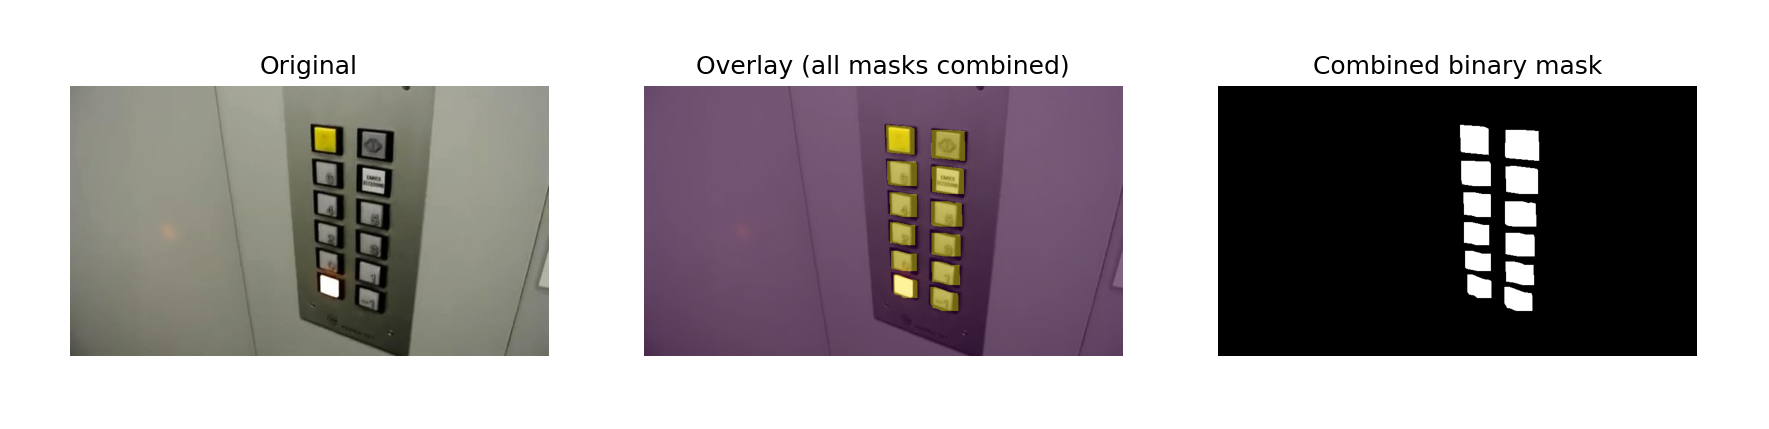
\includegraphics[width=0.95\textwidth]{figures/methodology/instances_Train_1349_1402__971.jpg.png}
    \caption{Example of an annotated image showing instance segmentation masks.}
    \label{fig:example_annotated_image}
\end{figure}

\section{Dataset quality assessment.}
\textbf{Note: This section is not done, and the text within it will most probably be changed drastically. However, I intent to keep structure and general idea the same.
One subsection for model assisted image quality assessment, and one for statistical image quality metrics.}

A systematic dataset quality assessment was performed to verify whether image-level degradation could negatively affect model performance.

\subsection{Statistical quality metrics.}
For every image, the following metrics were computed:
\begin{itemize}
    \item \textbf{Sharpness}, estimated using the variance of the Laplacian:
    \begin{equation}
        \sigma^2_{\text{lap}} = \mathrm{Var}(\nabla^2 I)
    \end{equation}
    where $I$ is the grayscale image.
    \item \textbf{Brightness}, defined as the mean grayscale intensity.
    \item \textbf{Edge density}, defined as the fraction of pixels with gradient magnitude above the 90th percentile.
\end{itemize}

% \paragraph{Results.}
% Figure~\ref{fig:quality_distributions} shows the distributions of sharpness, entropy, and brightness.
% The dataset exhibits predominantly well-exposed images with high information content and moderate sharpness.
% No distinct group of severely degraded images was observed.

% Figure~\ref{fig:quality_vs_performance} shows the relationship between image quality metrics and model performance.
% No strong correlation was found between sharpness or entropy and segmentation quality.
% False positives were primarily associated with low edge density, indicating visually ambiguous but valid scenes rather than image degradation.

% \paragraph{Conclusion.}
% The analysis indicates that dataset quality is high and does not constitute a limiting factor for model performance.
% Quality-based dataset pruning was therefore not applied.

---

\subsection{Model-assisted image assessment.}

In addition to image-level quality analysis, a model-assisted approach was used to identify potentially harmful training samples.

\paragraph{Method.}
A trained instance segmentation model was used to evaluate each training image individually.
For each image, the following metrics were computed:
\begin{itemize}
    \item Mean Intersection over Union:
    \begin{equation}
        \mathrm{IoU} = \frac{|M_{\text{pred}} \cap M_{\text{gt}}|}{|M_{\text{pred}} \cup M_{\text{gt}}|}
    \end{equation}
    \item Mean detection confidence:
    \begin{equation}
        \bar{c} = \frac{1}{N} \sum_{i=1}^{N} p_i
    \end{equation}
    where $p_i$ is the softmax score of the $i$-th predicted instance.
    \item Number of false positives and false negatives.
\end{itemize}

Images were ranked using a composite criterion favoring low \gls{iou}, high false positives, and high confidence incorrect predictions. Based on those criteria, a harm-score is measured,
based on which training set images are filtered and the potentially harmful ones are selected for manual inspection.

\paragraph{Inspection.}
Manual inspection of the lowest-ranked samples revealed two categories:
\begin{itemize}
    \item Hard but valid images (extreme viewpoints, zoom levels, or geometric distortions).
    \item Negative images without buttons, occasionally producing false positives.
\end{itemize}

After retraining the model with excluded possibly "harmful" samples, it was observed that removing hard samples reduced recall and segmentation accuracy, while removing a small number of negative samples slightly improved precision.

% \paragraph{Conclusion.}
% Most samples identified as potentially harmful were informative hard examples that improved generalization.
% The final model was therefore trained on the full dataset, excluding only a small number of negative images without annotated buttons.


\section{Model architectures and training strategy}

Two instance segmentation model families are employed in this project, each serving
a distinct role within the overall perception pipeline. \gls{maskrcnn} is used as a
high-accuracy reference model and as the backbone of the semi-automatic annotation
workflow (Section~3.3), while \gls{yolo}v8-Seg is trained and evaluated as a
deployment-oriented solution suitable for embedded hardware.

\subsection*{Common training strategy}

All models are trained using a transfer learning approach. Networks are initialized
from pretrained checkpoints and fine-tuned on the project-specific dataset, rather
than being trained from scratch. This strategy improves convergence speed and
generalization performance, particularly given the moderate dataset size.

The dataset is split into training and validation subsets using an 80/20 ratio with
a fixed random seed (42) to ensure reproducibility. Standard data augmentation
techniques are applied during training to improve robustness to viewpoint and
lighting variations. These include random horizontal flipping with probability
$p=0.5$ and color jitter with brightness, contrast, and saturation factors set to
0.1.

\subsection*{Mask R-CNN training}

\gls{maskrcnn} is trained using a custom PyTorch-based pipeline with \gls{coco}-formatted
instance annotations. Training is performed for 50 epochs with a batch size of 2,
reflecting the higher memory requirements of region-based instance segmentation
models.

Optimization is performed using the AdamW optimizer with a learning rate of
$5 \times 10^{-4}$ and weight decay of $1 \times 10^{-4}$. A ReduceLROnPlateau learning
rate scheduler is employed, reducing the learning rate by a factor of 0.5 when the
validation loss does not improve for three consecutive epochs. Early stopping is
enabled with a patience of 10 epochs based on validation loss.

\gls{maskrcnn} is retrained iteratively as the annotated dataset grows. This iterative
training is applied exclusively to the \gls{maskrcnn} model, as it is used to generate
pre-annotations during the semi-automatic annotation process. Model checkpoints are
created after approximately 100, 450, and 900 annotated training images, enabling
progressively improved annotation quality and reduced manual correction effort.

\subsection*{YOLOv8-Seg training}

\gls{yolo}v8-Seg is trained using the Ultralytics framework with the pretrained
\texttt{yolov8s-seg.pt} checkpoint. Training is performed for 50 epochs with a batch
size of 8 and an input resolution of $640 \times 640$ pixels. The default Ultralytics hyperparameters are used for the training.
Early stopping patience is set to 10 epochs based on validation loss. 3 epochs for learning rate warmup, gradually increasing the learning rate from a low value to the initial learning rate to stabilize training early on

Unlike \gls{maskrcnn}, \gls{yolo}v8-Seg is not retrained iteratively during annotation. Instead,
it is trained on the finalized annotated dataset and evaluated as a candidate model
for real-time deployment on embedded hardware.

\subsection*{Loss functions and optimization objectives}

Both instance segmentation models are trained by minimizing a composite loss
function that jointly optimizes object classification, localization, and mask
prediction. Although \gls{maskrcnn} and \gls{yolo}v8-Seg differ architecturally, their
optimization objectives are conceptually aligned.

\paragraph{Mask R-CNN.}
The training objective of \gls{maskrcnn} is defined as a multi-task loss composed of
three terms \citep{he2017maskrcnn}:
\begin{equation}
\mathcal{L}_{\text{Mask R-CNN}} =
\mathcal{L}_{\text{cls}} +
\mathcal{L}_{\text{box}} +
\mathcal{L}_{\text{mask}},
\end{equation}
where $\mathcal{L}_{\text{cls}}$ denotes the classification loss, implemented as
categorical cross-entropy; $\mathcal{L}_{\text{box}}$ represents bounding-box
regression using the smooth $L_1$ loss; and $\mathcal{L}_{\text{mask}}$ is a
pixel-wise binary cross-entropy loss applied to each predicted instance mask.

\paragraph{YOLOv8-Seg.}
\gls{yolo}v8-Seg integrates detection and segmentation into a single-stage architecture.
The total training loss is expressed as a weighted sum of classification,
localization, and segmentation losses \citep{jocher2023yolov8}:
\begin{equation}
\mathcal{L}_{\text{YOLO}} =
\lambda_{\text{cls}} \mathcal{L}_{\text{cls}} +
\lambda_{\text{box}} \mathcal{L}_{\text{box}} +
\lambda_{\text{seg}} \mathcal{L}_{\text{seg}},
\end{equation}
where $\mathcal{L}_{\text{seg}}$ represents the segmentation loss applied to the
predicted mask outputs, and the weighting coefficients $\lambda$ control the
relative contribution of each task during optimization.

Despite architectural differences, both models optimize comparable objectives,
enabling consistent evaluation of segmentation accuracy and computational
efficiency across reference and deployment-oriented architectures.

\subsection*{OCR-based button interpretation}

Following instance segmentation, the detected button regions are passed to a
semantic interpretation stage. Segmented button instances are cropped and processed
by an \gls{ocr}-based recognition module to extract character labels or symbols associated
with each button. This stage enables the robot to associate detected interaction
points with their functional meaning and supports downstream decision-making during
autonomous operation.


\section{Evaluation metrics and methodology}

The performance of the instance segmentation models is evaluated using a combination
of standard \gls{coco} metrics and task-oriented instance-level metrics. This dual
evaluation strategy allows both standardized benchmarking and direct assessment of
model suitability for robotic interaction tasks.

\subsection{Intersection over Union}

Segmentation quality is measured using Intersection over Union (\gls{iou}). For a
predicted instance mask $M_p$ and the corresponding ground-truth mask $M_{gt}$, \gls{iou}
is defined as:

\begin{equation}
\mathrm{IoU} = \frac{|M_p \cap M_{gt}|}{|M_p \cup M_{gt}|}
\end{equation}

\gls{iou} values range from 0 (no overlap) to 1 (perfect overlap). In this project, \gls{iou} is
computed at the instance level and used both for matching predicted and ground-truth
instances and for computing summary statistics.

\subsection{Precision, recall, and F1-score}

Instance-level detection performance is quantified using precision, recall, and
F1-score. A predicted instance is considered a true positive if its \gls{iou} with an
unmatched ground-truth instance exceeds a threshold of 0.5. Precision and recall
are defined as:

\begin{equation}
\mathrm{Precision} = \frac{TP}{TP + FP}
\end{equation}

\begin{equation}
\mathrm{Recall} = \frac{TP}{TP + FN}
\end{equation}

where $TP$, $FP$, and $FN$ denote the number of true positives, false positives, and
false negatives, respectively.

The F1-score, which balances precision and recall, is computed as:

\begin{equation}
\mathrm{F1} = \frac{2 \cdot \mathrm{Precision} \cdot \mathrm{Recall}}
{\mathrm{Precision} + \mathrm{Recall}}
\end{equation}

These metrics provide intuitive insight into detection reliability and are
particularly relevant for robotic interaction tasks, where both missed detections
and false positives can lead to failed interactions.

\subsection{Average Precision under the COCO protocol}

To enable standardized benchmarking, model performance is additionally evaluated
using the \gls{coco} instance segmentation protocol. Average Precision (\gls{ap}) is computed
as the area under the precision--recall curve:

\begin{equation}
\mathrm{AP} = \int_{0}^{1} p(r)\,dr
\end{equation}

where $p(r)$ denotes precision as a function of recall $r$. Following the \gls{coco}
evaluation methodology, \gls{ap} is reported as the mean over multiple \gls{iou} thresholds
ranging from 0.50 to 0.95 in increments of 0.05. Additional metrics such as
$\mathrm{AP}_{50}$ and $\mathrm{AP}_{75}$ are also reported to provide insight into
performance at specific overlap thresholds.

\subsection{Mean IoU and runtime performance}

For correctly matched instances, the mean \gls{iou} is computed across the test set to
assess overall segmentation accuracy. In addition to accuracy metrics, runtime
performance is measured by recording per-image inference time. Average inference
time and frames per second (\gls{fps}) are reported to evaluate suitability for real-time
deployment on embedded hardware.

\subsection{Evaluation protocol}

All evaluations are conducted on a held-out test set that is not used during
training or validation. Identical datasets, matching criteria, and thresholds are
used across all model architectures to ensure fair comparison. \gls{coco}-based metrics
are computed using the official evaluation tools, while precision, recall, F1-score,
mean \gls{iou}, and runtime statistics are computed using a custom evaluation pipeline.

The evaluation methodology described in this section forms the basis for the
quantitative comparison of models presented in Chapter~4.

\section{Embedded deployment and optimization}

\begin{wrapfigure}{r}{0.42\textwidth}
    \centering
    \vspace{-10pt}
    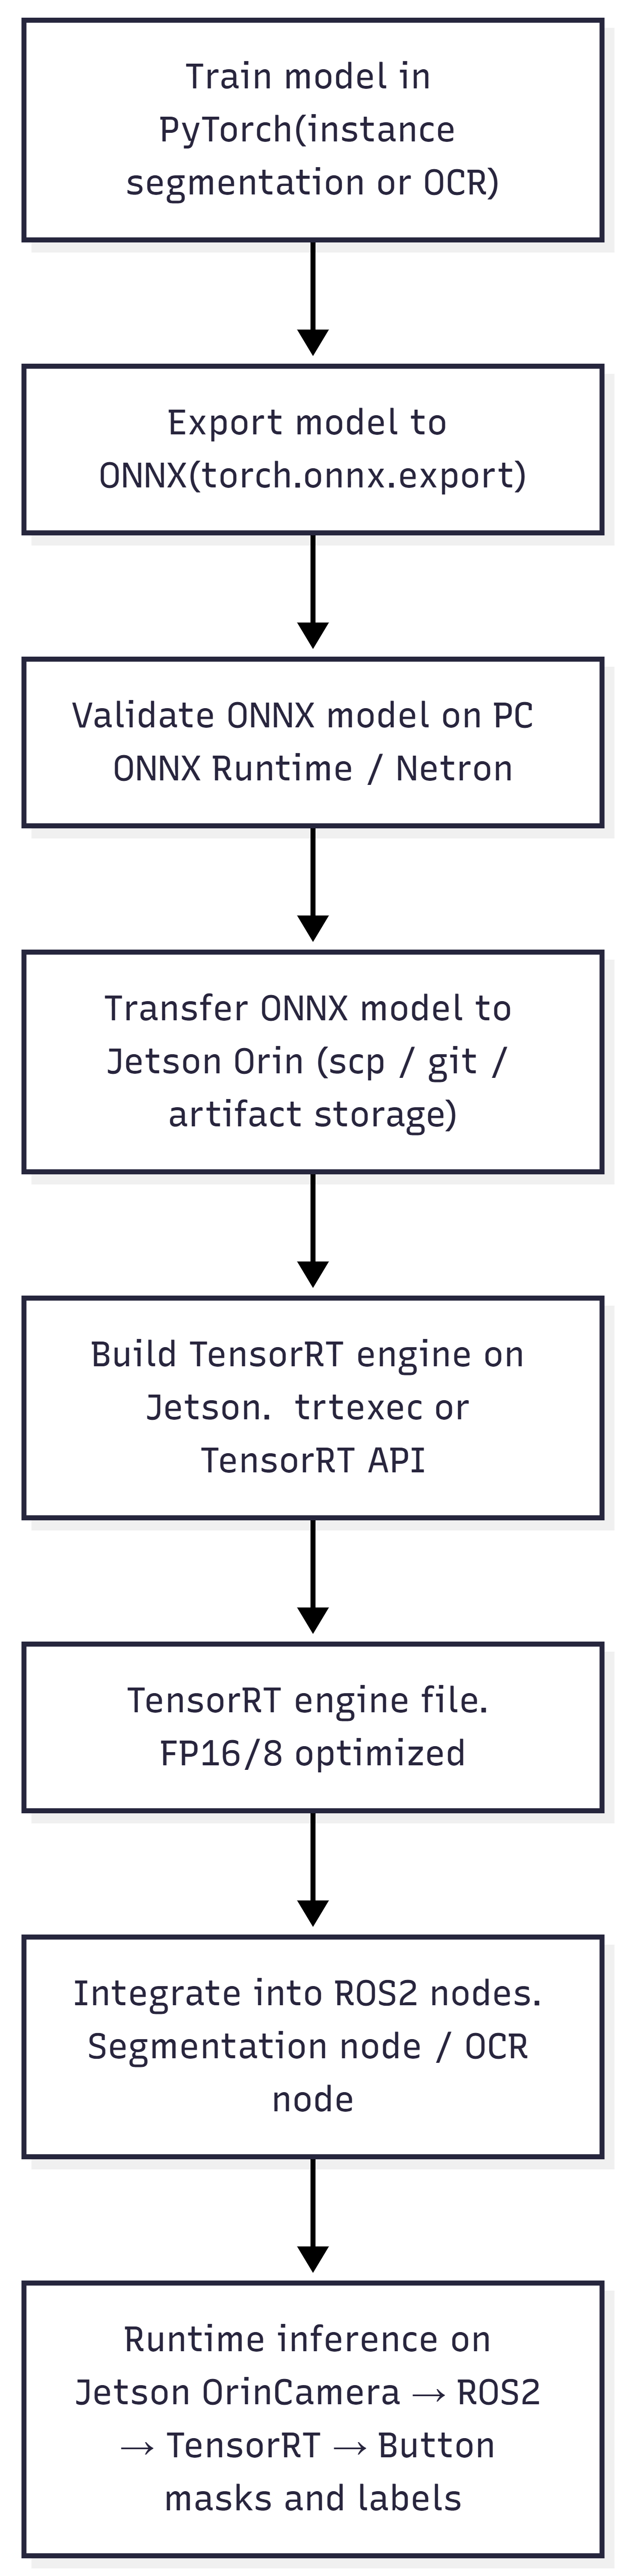
\includegraphics[width=0.25\textwidth]{figures/methodology/Embedded_workflow.png}
    \captionsetup{width=0.3\textwidth}
    \caption{Deployment and optimization workflow for 
    models on \gls{jetson} Orin using \gls{onnx} and \gls{tensorrt}.}
    \label{fig:tensorrt_workflow}
    \vspace{-10pt}
\end{wrapfigure}

To enable real-time execution on embedded hardware, and wrap up step 1 of the workflow strategy in Figure~\ref{fig:scalable_workflow}, trained models are optimized
and deployed on a \gls{jetson} Orin platform. The deployment workflow is designed
to be identical for both the instance segmentation model and the OCR-based button
classification model.

Models are first trained in PyTorch and exported to the Open Neural Network Exchange
(\gls{onnx}) \citep{onnx2019} format. The exported \gls{onnx} models are validated on a desktop system using \gls{onnx}
Runtime and model inspection tools to ensure numerical correctness and structural
compatibility prior to deployment.

Validated \gls{onnx} models are then transferred to the \gls{jetson} Orin device, where
\gls{tensorrt} is used to build optimized inference engines. Engine generation is
performed directly on the target device to ensure compatibility with the specific
\gls{gpu} architecture. \gls{fp16} precision is used to reduce memory footprint and improve
inference speed while maintaining sufficient numerical accuracy.

The resulting \gls{tensorrt} engines are integrated into \gls{ros2} nodes responsible for
perception tasks. At runtime, image data from the \gls{rgbd} camera is passed through
the \gls{ros2} pipeline and processed by the \gls{tensorrt} engines to produce instance
segmentation masks and corresponding button labels.

The complete deployment and optimization workflow is illustrated in
Figure~\ref{fig:tensorrt_workflow}. This approach ensures a consistent and efficient
deployment pipeline and enables fair evaluation of different model architectures
under identical runtime constraints.


\chapter{Results}
\label{ch:results}

This chapter presents the quantitative results obtained for the main technical
components of the proposed elevator-interaction pipeline. The current version of
the report focuses on the visual detection subsystem based on \gls{yolo}
instance segmentation and the \gls{ocr}-based button interpretation stage. Unless
stated otherwise, final model comparisons are
reported on held-out test sets, while model selection during training and
hyperparameter tuning is based on the validation split.

\section{YOLO hyperparameter tuning and evaluation}

\subsection{Baseline YOLOv8-Seg performance}

The baseline \gls{yolo}v8-Seg model trained on \texttt{elevator\_split} established
the main reference point for all subsequent experiments. On the validation split,
the best checkpoint was obtained at epoch 49. This model achieved a mask
$\mathrm{mAP}_{50}$ of 0.93931 and a mask
$\mathrm{mAP}_{50\text{:}95}$ of 0.59645, with mask precision and recall of
0.90623 and 0.89947, respectively. These results confirmed that the initial
configuration was already strong enough to serve as a realistic benchmark rather
than only as a preliminary starting point.

When evaluated on the held-out original test split at an image size of 640 pixels,
the same baseline model achieved a mask $\mathrm{mAP}_{50}$ of 0.91921 and a mask
$\mathrm{mAP}_{50\text{:}95}$ of 0.58295. This test result is slightly lower than the
best validation value, which is expected, but it still indicates good
generalization to unseen elevator-panel images.

\subsection{Hyperparameter tuning results}

The three-stage hyperparameter tuning procedure improved validation performance,
but the gains were moderate. Stage 1 served as a narrow Ray Tune search around
the baseline configuration. As shown in Figure~\ref{fig:stage1_mask_map}, most of
the displayed Stage 1 trials did not produce meaningful mask performance.
Among the first ten runs shown in the \gls{wandb} export, only three
configurations reached non-zero $\mathrm{mAP}_{50\text{:}95}$ values, while the
remaining trials stayed at zero throughout the 30-epoch search horizon. These
zero-valued runs still count as valid tuning outcomes because they identify
unsuccessful regions of the hyperparameter space. The main conclusion from Stage
1 was therefore not that tuning broadly improved all runs, but that only a small
subset of configurations was suitable for further evaluation in Stage 2.

\begin{figure}[htbp]
    \centering
    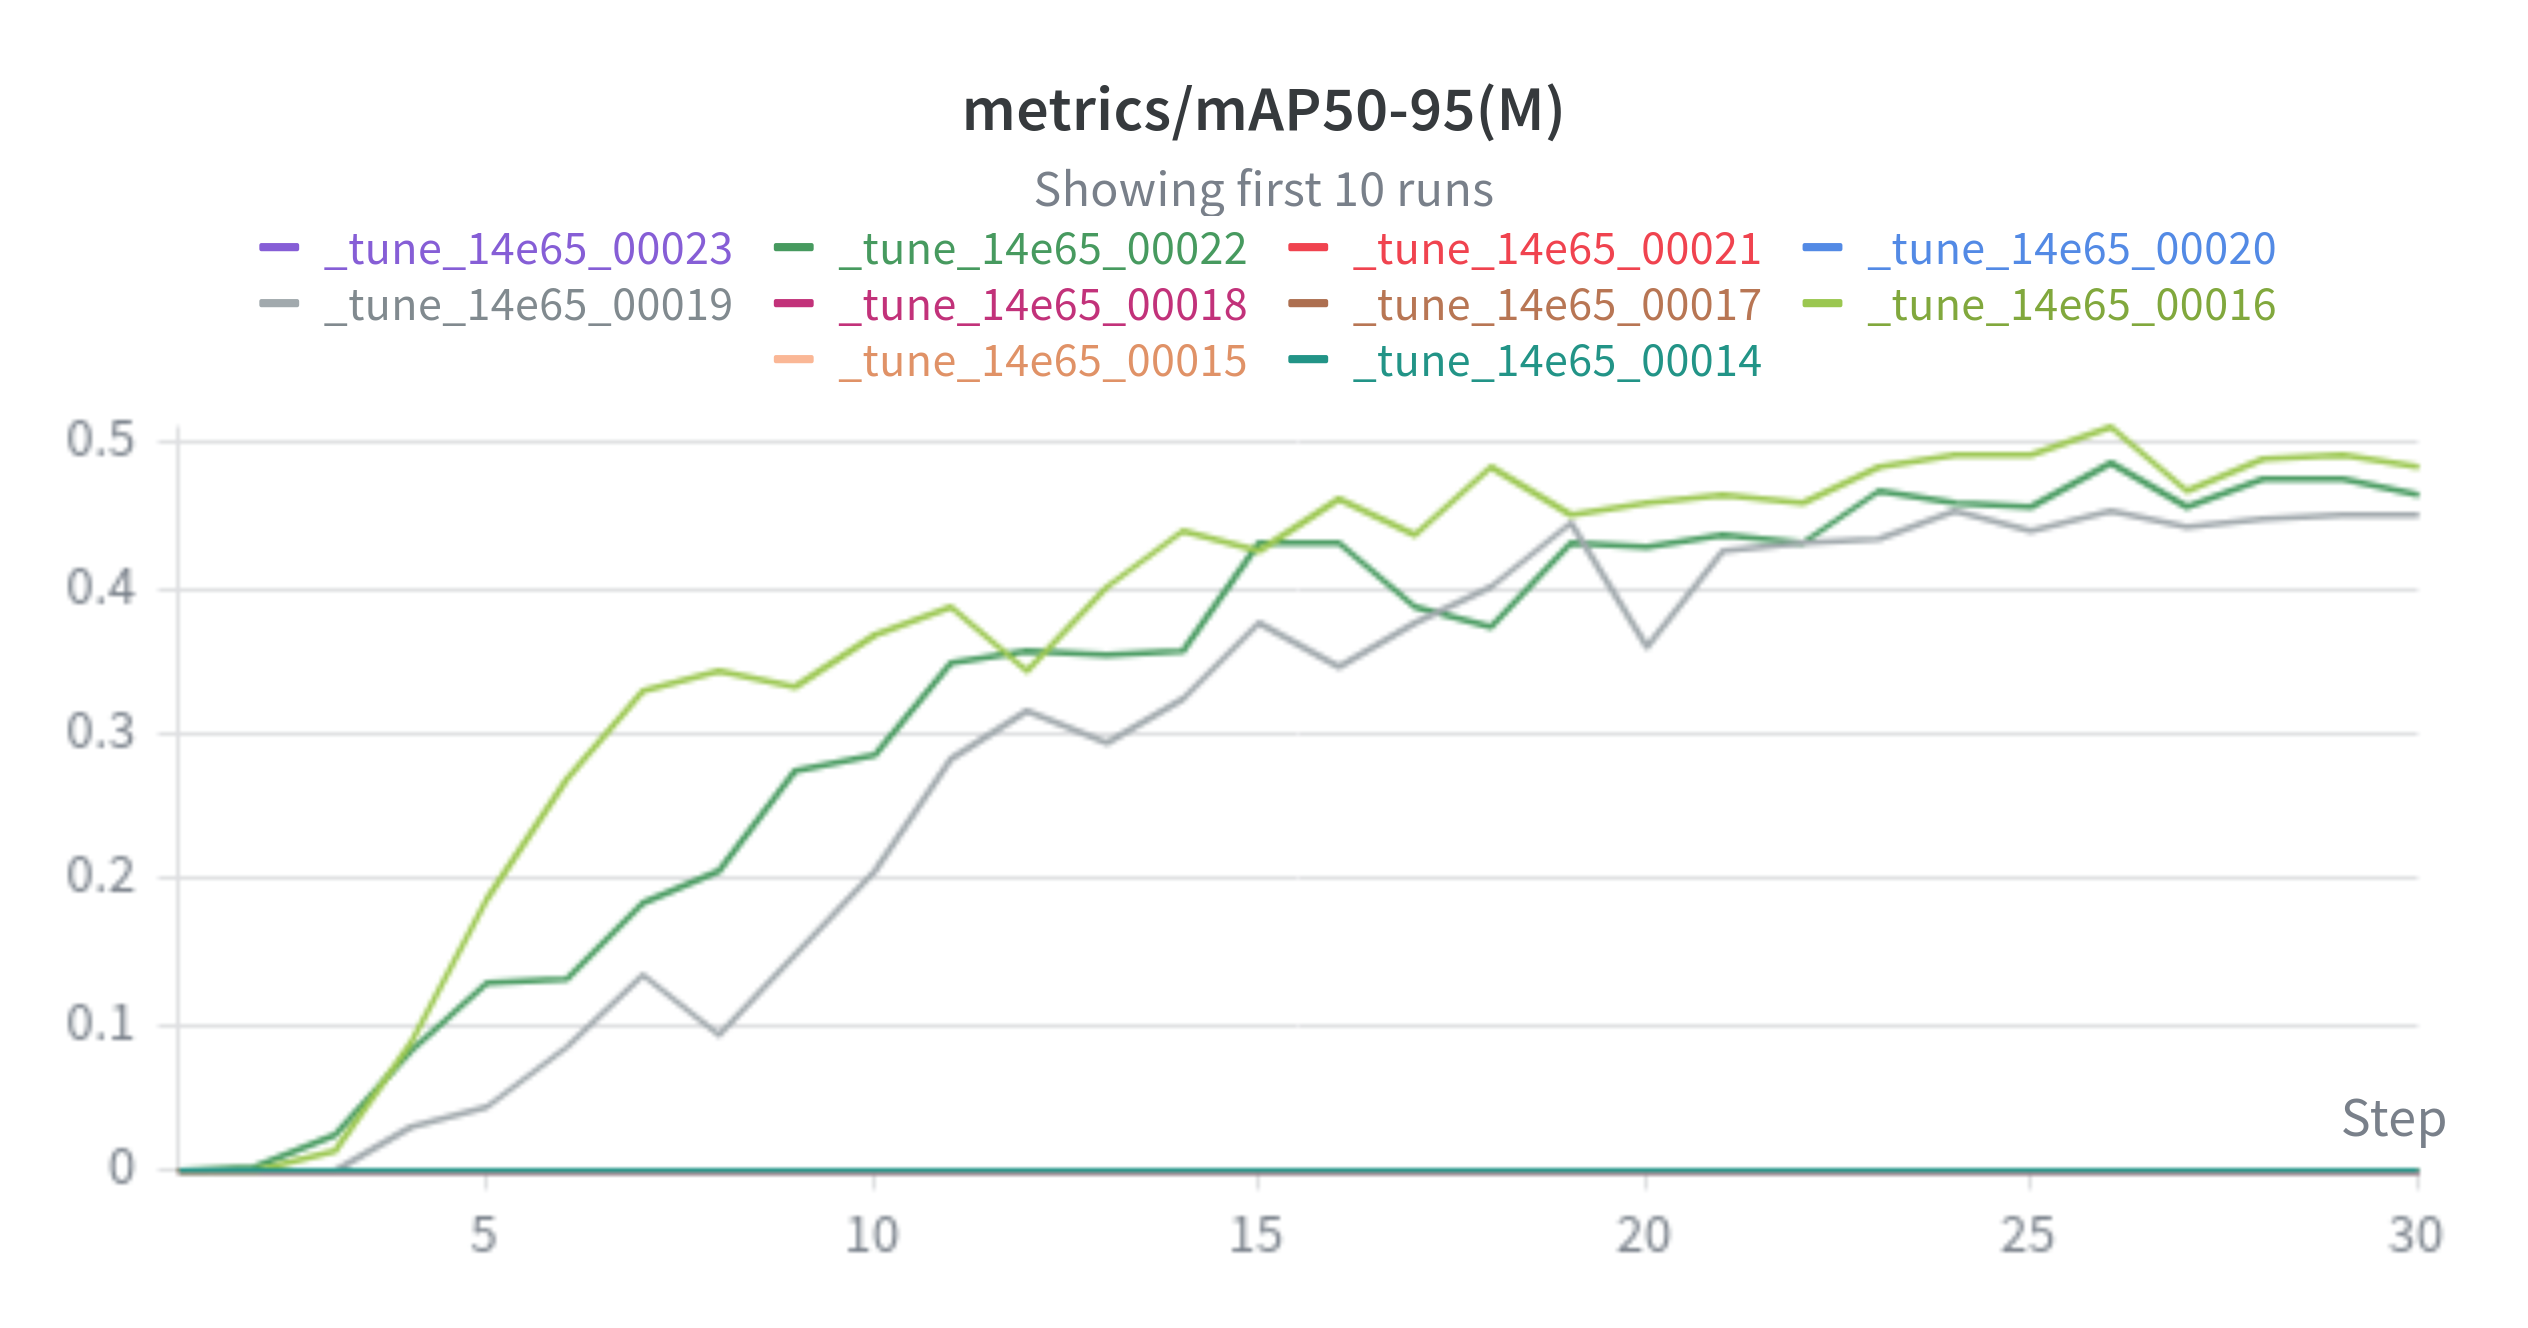
\includegraphics[width=0.82\textwidth]{figures/results/stage1_yolo_mAP50-95_M.png}
    \caption{Stage 1 validation mask $\mathrm{mAP}_{50\text{:}95}$ for the first ten runs shown in the \gls{wandb} sweep export. Only a small subset of configurations produced non-zero validation performance.}
    \label{fig:stage1_mask_map}
\end{figure}

The most relevant outcome of the tuning pipeline was that the best Stage 2
configuration consistently selected a batch size of 16 and an input resolution of
768 pixels. Stage 3 then resumed training from this configuration with a reduced
initial learning rate.

Figure~\ref{fig:stage2_mask_map} shows the broader Stage 2 validation mask
$\mathrm{mAP}_{50\text{:}95}$ trends. In contrast to Stage 1, Stage 2 produced a
larger number of usable configurations because the search was restricted to the
top Stage 1 candidates and only varied image size and batch size. The logged
results show that eight out of sixteen unique Stage 2 configurations achieved
non-zero mask $\mathrm{mAP}_{50\text{:}95}$ values. Most successful runs were
observed at an input resolution of 640 pixels, while many 768-pixel variants
remained unsuccessful. The main exception was the
\texttt{cfg1\_b16\_sz768} configuration, which produced the best Stage 2 result
and was therefore selected for Stage 3 refinement.

\begin{figure}[htbp]
    \centering
    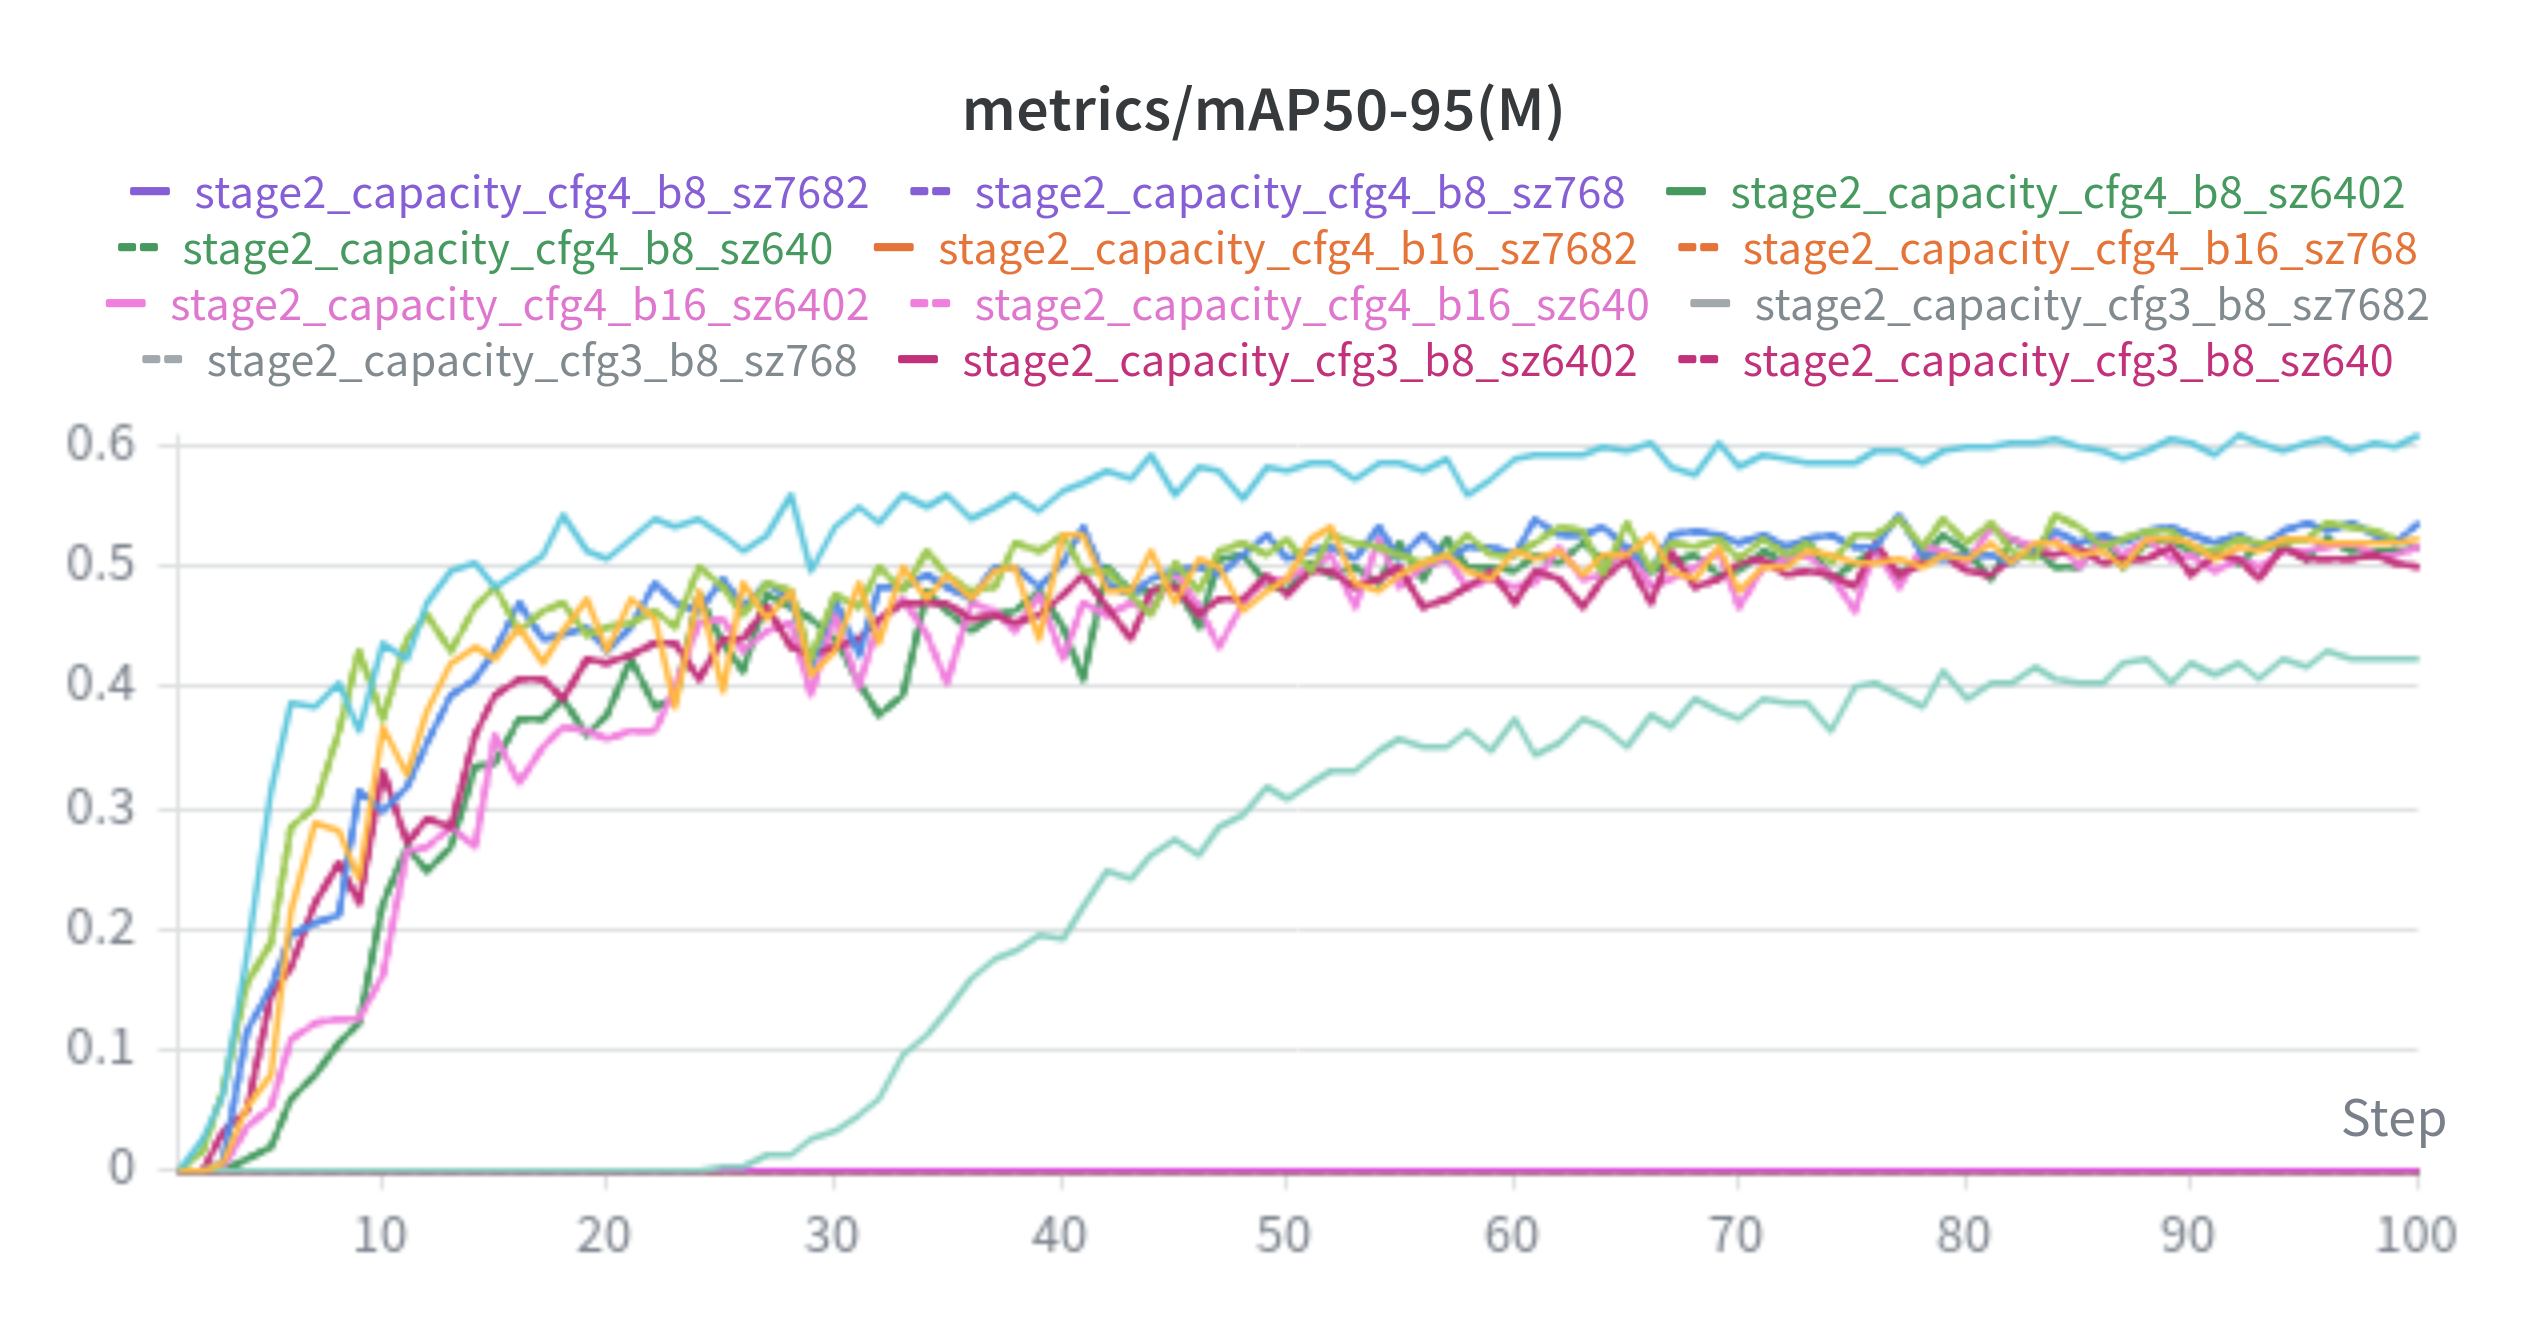
\includegraphics[width=0.82\textwidth]{figures/results/stage2_yolo_mAP50-95_m_full.png}
    \caption{Stage 2 validation mask $\mathrm{mAP}_{50\text{:}95}$ for the broader set of capacity-tuning runs. Compared with Stage 1, more configurations produced usable validation performance, although unsuccessful runs were still present.}
    \label{fig:stage2_mask_map}
\end{figure}

Table~\ref{tab:yolo_tuning_results} summarizes the best validation results of the
baseline model and the best Stage 3 tuned model. The tuned model reached its best
validation performance at epoch 120 and improved mask
$\mathrm{mAP}_{50\text{:}95}$ from 0.59645 to 0.63064. This corresponds to an absolute
gain of 0.03419 on the validation set. Precision changed only slightly, while
recall increased from 0.89947 to 0.90810, indicating that the tuned model mainly
benefited from better localization and mask quality rather than from a major shift
in confidence calibration. This improvement, however, should be interpreted as a
validation-stage model-selection result and not as evidence that the tuned model
outperformed the baseline on the final held-out test set.

Figures~\ref{fig:stage3_mask_map} and \ref{fig:stage3_val_seg_loss} show the
behavior of the two Stage 3 refinement runs. Both runs followed almost identical
validation trajectories, which indicates that the refinement step was stable once
the best Stage 2 configuration had been selected. The validation mask
$\mathrm{mAP}_{50\text{:}95}$ increased rapidly in the early epochs and then
stabilized slightly above 0.62. At the same time, the validation segmentation
loss dropped sharply at the start of training and then remained close to a stable
plateau. These curves indicate a controlled refinement of an already strong
configuration rather than a major qualitative change in optimization behavior.

\begin{figure}[htbp]
    \centering
    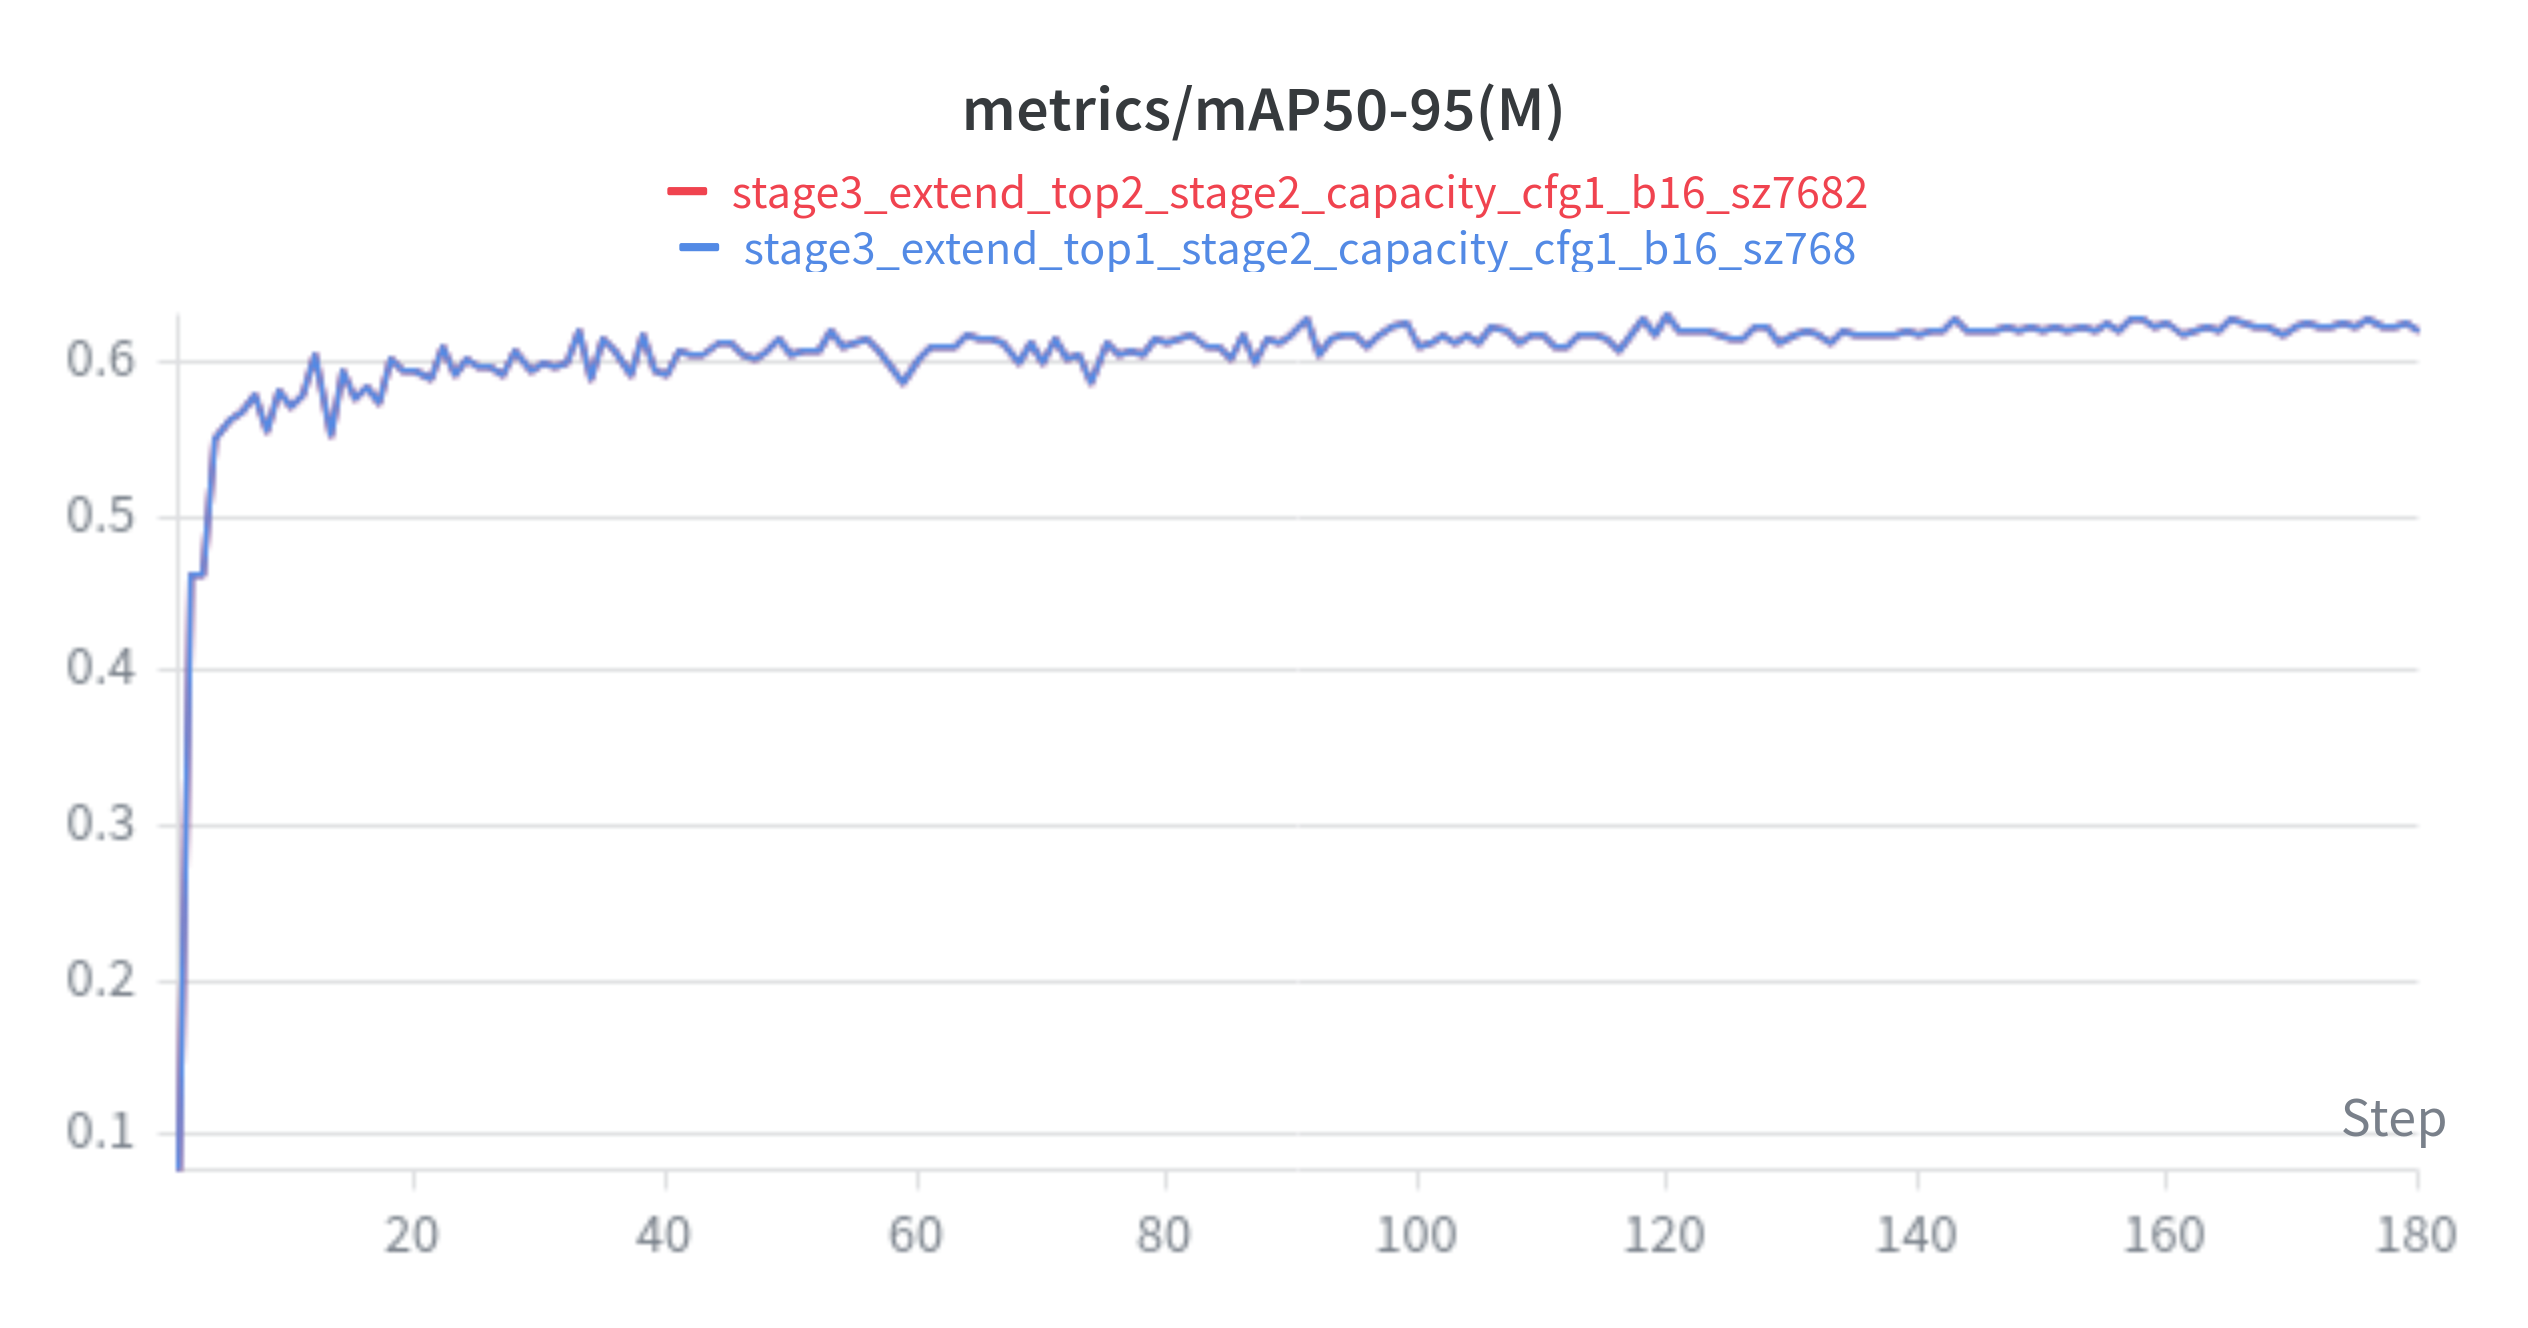
\includegraphics[width=0.82\textwidth]{figures/results/stage3_yolo_mAP50-95_M.png}
    \caption{Stage 3 validation mask $\mathrm{mAP}_{50\text{:}95}$ for the two refinement runs. The runs followed nearly identical trajectories and converged to the same performance region.}
    \label{fig:stage3_mask_map}
\end{figure}

\begin{figure}[htbp]
    \centering
    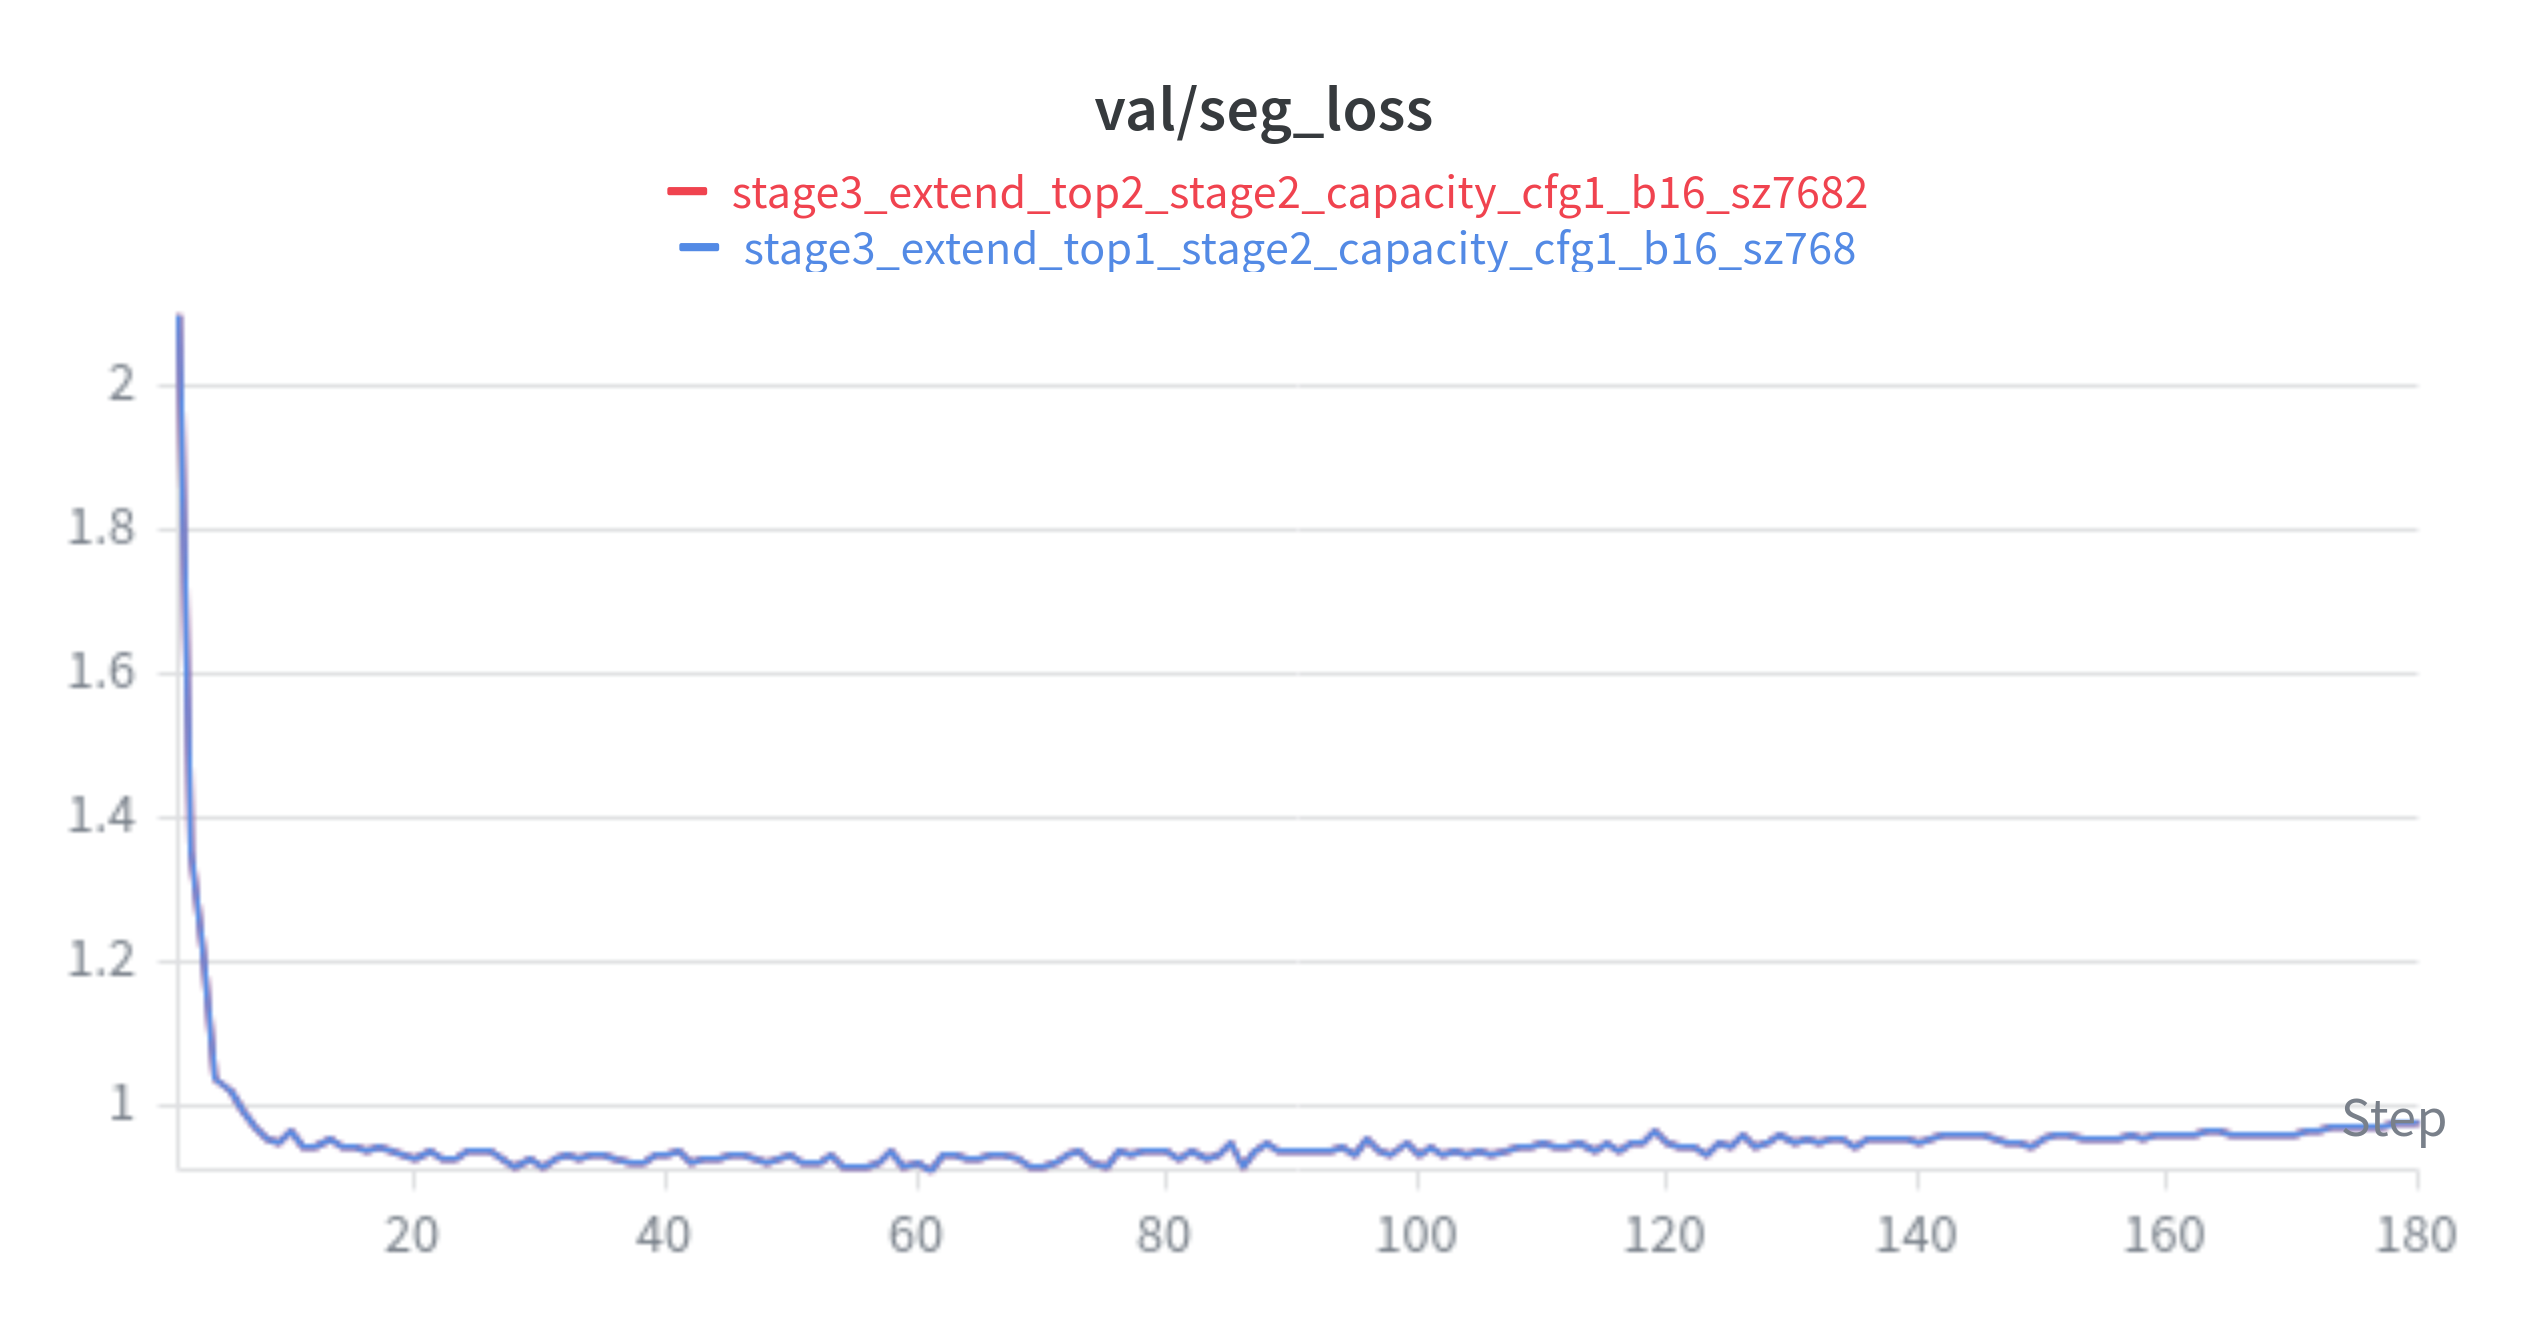
\includegraphics[width=0.82\textwidth]{figures/results/stage3_yolo_seg_loss_val.png}
    \caption{Stage 3 validation segmentation loss. After a steep initial decrease, the loss remained stable, indicating consistent convergence during refinement.}
    \label{fig:stage3_val_seg_loss}
\end{figure}

\begin{table}[htbp]
    \centering
    \caption{Best validation results of the baseline and tuned \gls{yolo}v8-Seg models.}
    \label{tab:yolo_tuning_results}
    \small
    \begin{tabular}{lccccc}
        \toprule
        Model & Best epoch & Mask $\mathrm{mAP}_{50}$ & Mask $\mathrm{mAP}_{50\text{:}95}$ & Mask precision & Mask recall \\
        \midrule
        Baseline YOLOv8-Seg & 49 & 0.93931 & 0.59645 & 0.90623 & 0.89947 \\
        Stage 3 tuned YOLOv8-Seg & 120 & 0.94268 & 0.63064 & 0.90150 & 0.90810 \\
        \bottomrule
    \end{tabular}
\end{table}

\begin{table}[htbp]
    \centering
    \caption{Held-out test-set comparison between the baseline and the selected Stage 3 tuned \gls{yolo}v8-Seg model.}
    \label{tab:yolo_tuning_test_results}
    \small
    \begin{tabular}{lccccc}
        \toprule
        Model & Image size & Mask $\mathrm{mAP}_{50}$ & Mask $\mathrm{mAP}_{50\text{:}95}$ & Mask precision & Mask recall \\
        \midrule
        Baseline YOLOv8-Seg & 640 & 0.92819 & 0.73744 & 0.87603 & 0.90832 \\
        Stage 3 tuned YOLOv8-Seg & 640 & 0.91706 & 0.68829 & 0.86839 & 0.88443 \\
        Baseline YOLOv8-Seg & 768 & 0.92638 & 0.74752 & 0.86778 & 0.92329 \\
        Stage 3 tuned YOLOv8-Seg & 768 & 0.92719 & 0.71985 & 0.87399 & 0.90724 \\
        \bottomrule
    \end{tabular}
\end{table}

These results show that systematic hyperparameter tuning was useful for improving
validation performance. However, the held-out test comparison in
Table~\ref{tab:yolo_tuning_test_results} does not support replacing the baseline
checkpoint with the Stage 3 model. At an image size of 640 pixels, the baseline
outperformed the tuned model by 0.04915 mask $\mathrm{mAP}_{50\text{:}95}$, and
at 768 pixels the margin remained 0.02767 in favor of the baseline. For this
reason, the original baseline checkpoint remained the reference model for the
later deployment-oriented experiments and for the final adaptation study.

\subsection{Comparison with YOLO26}

To evaluate whether a newer Ultralytics architecture could provide a better
segmentation model under comparable conditions, YOLO26-small was trained using
the same baseline recipe and later extended to a longer 180-epoch run. The final
comparison was performed on the held-out original test split at image sizes of 640
and 768 pixels.

The results are presented in Table~\ref{tab:yolo26_comparison}. At an image size
of 640 pixels, the baseline \gls{yolo}v8-Seg model achieved a mask
$\mathrm{mAP}_{50\text{:}95}$ of 0.58295, whereas YOLO26 reached 0.57538. At 768
pixels, the baseline again remained slightly better, with 0.62325 compared with
0.61689 for YOLO26. The higher-resolution evaluation benefited both models, but it
did not change the ranking between them. Under the training and evaluation
conditions used in this project, YOLO26 therefore did not outperform the baseline
\gls{yolo}v8-Seg model on the held-out test set.

Figure~\ref{fig:yolo26_mask_map} shows the corresponding validation mask
$\mathrm{mAP}_{50\text{:}95}$ curves for the two YOLO26 runs. Extending the
training to 180 epochs shifted the validation curve upward and produced a higher
plateau than the shorter run. However, the improvement remained modest and was
not sufficient to reverse the final test-set ranking against the baseline
\gls{yolo}v8-Seg model.

\begin{table}[htbp]
    \centering
    \caption{Test-set comparison between the baseline \gls{yolo}v8-Seg model and YOLO26-small.}
    \label{tab:yolo26_comparison}
    \small
    \begin{tabular}{lccccc}
        \toprule
        Model & Image size & Mask $\mathrm{mAP}_{50}$ & Mask $\mathrm{mAP}_{50\text{:}95}$ & Mask precision & Mask recall \\
        \midrule
        YOLOv8-Seg baseline & 640 & 0.91921 & 0.58295 & 0.86835 & 0.89896 \\
        YOLO26-small & 640 & 0.91209 & 0.57538 & 0.87300 & 0.89879 \\
        YOLOv8-Seg baseline & 768 & 0.92384 & 0.62325 & 0.86577 & 0.91939 \\
        YOLO26-small & 768 & 0.92596 & 0.61689 & 0.88408 & 0.91326 \\
        \bottomrule
    \end{tabular}
\end{table}

\begin{figure}[htbp]
    \centering
    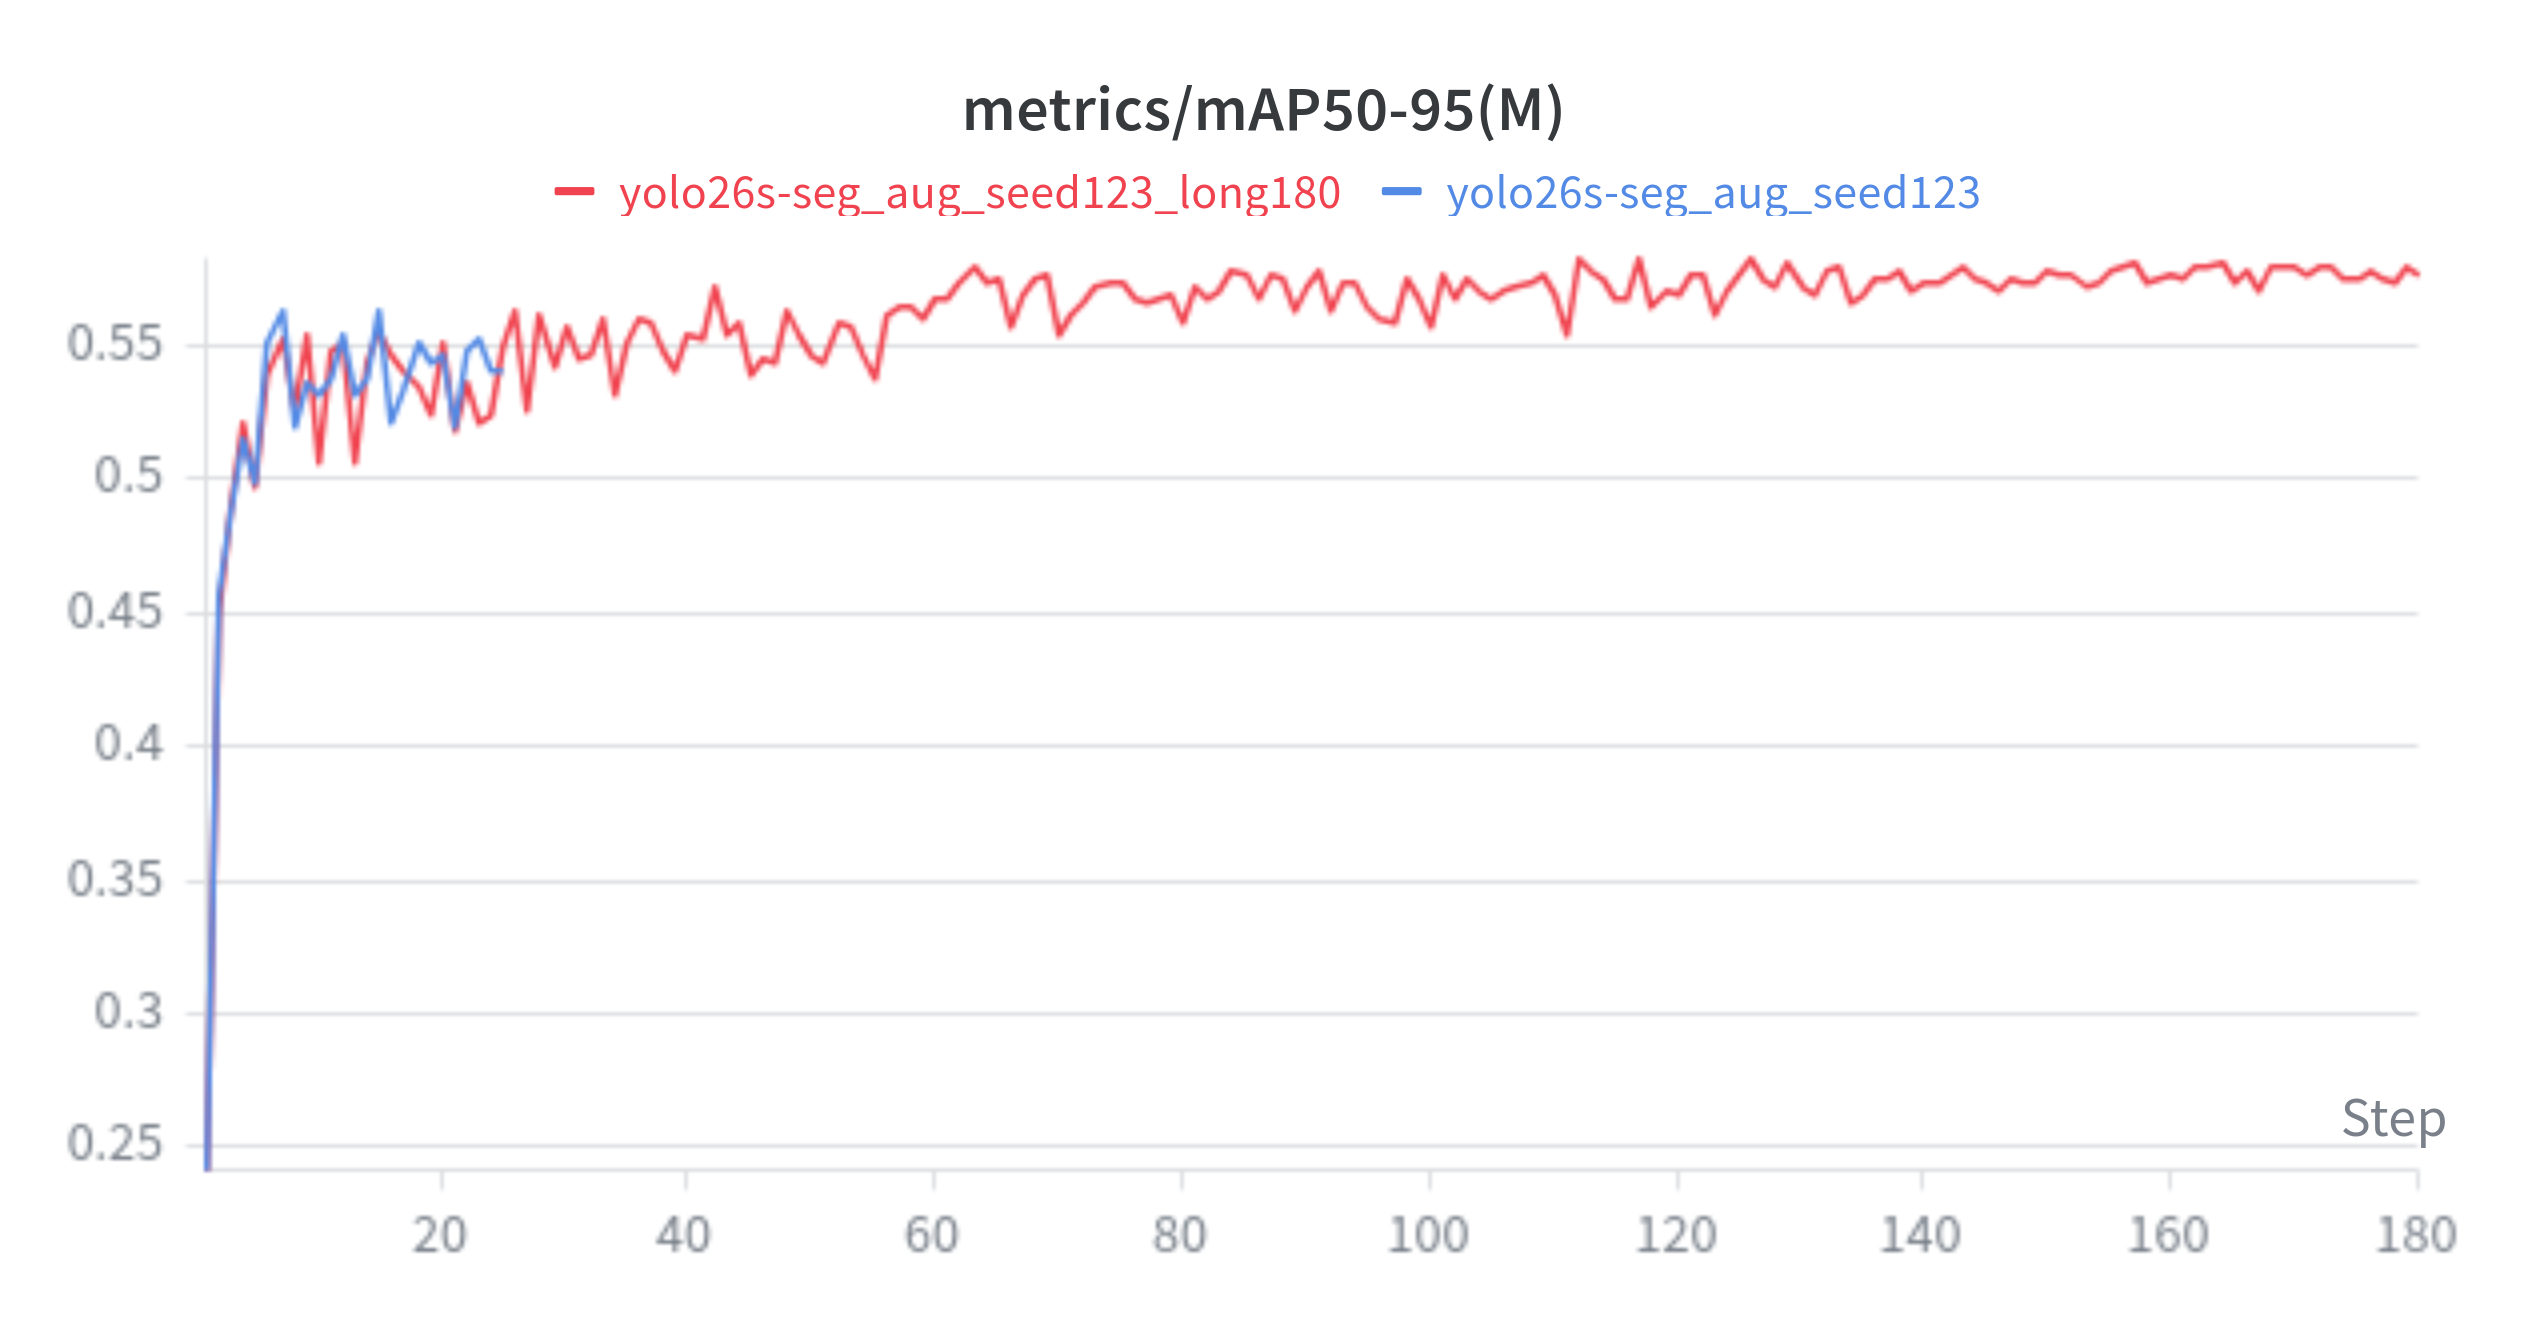
\includegraphics[width=0.82\textwidth]{figures/results/yolo26_mAP50-95_M.png}
    \caption{Validation mask $\mathrm{mAP}_{50\text{:}95}$ for the two YOLO26 training runs. The longer 180-epoch run improved over the shorter run, but the resulting model still did not surpass the YOLOv8 baseline on the held-out test set.}
    \label{fig:yolo26_mask_map}
\end{figure}

\subsection{Environment-specific fine-tuning with \gls{adc} data}

The final \gls{yolo} experiment focused on adaptation to the target university
environment. For this purpose, the baseline checkpoint was fine-tuned on a mixed
dataset that combined the original elevator-panel dataset with 46 newly
collected and annotated images from HAN University, Building 31. This building
served as the pilot environment for planned robot deployment tests. The
environment-specific images were collected with the \gls{adc} and then split into
32 training images, 7 validation images, and 7 test images before being merged
with the original dataset. The resulting evaluation therefore makes it possible
to determine whether the adapted model improves in the target environment without
losing too much performance on the original domain.

Table~\ref{tab:adc_original_test} shows the results on the original held-out test
split. The fine-tuned model remained effectively tied with the baseline. Its mask
$\mathrm{mAP}_{50\text{:}95}$ changed from 0.58295 to 0.58293, which is
negligible. The box metrics improved slightly, and mask precision and recall also
increased marginally. This indicates that adaptation to the new environment did
not cause a meaningful degradation on the original dataset.

The corresponding validation curve is shown in
Figure~\ref{fig:adc_finetune_mask_map}. The fine-tuned model remained in the same
overall validation range as the original baseline, with modest fluctuations
around 0.58. This is consistent with the final original-test comparison, which
showed that the fine-tuned model preserved the baseline's general performance
while becoming substantially more effective on the environment-specific
\texttt{adc\_first} test set.

\begin{table}[htbp]
    \centering
    \caption{Performance on the original held-out elevator test split before and after \gls{adc} fine-tuning.}
    \label{tab:adc_original_test}
    \small
    \begin{tabular}{lcccc}
        \toprule
        Model & Mask $\mathrm{mAP}_{50}$ & Mask $\mathrm{mAP}_{50\text{:}95}$ & Mask precision & Mask recall \\
        \midrule
        Baseline YOLOv8-Seg & 0.91921 & 0.58295 & 0.86835 & 0.89896 \\
        \glsentryshort{adc} fine-tuned YOLOv8-Seg & 0.91912 & 0.58293 & 0.88043 & 0.90050 \\
        \bottomrule
    \end{tabular}
\end{table}

\begin{figure}[htbp]
    \centering
    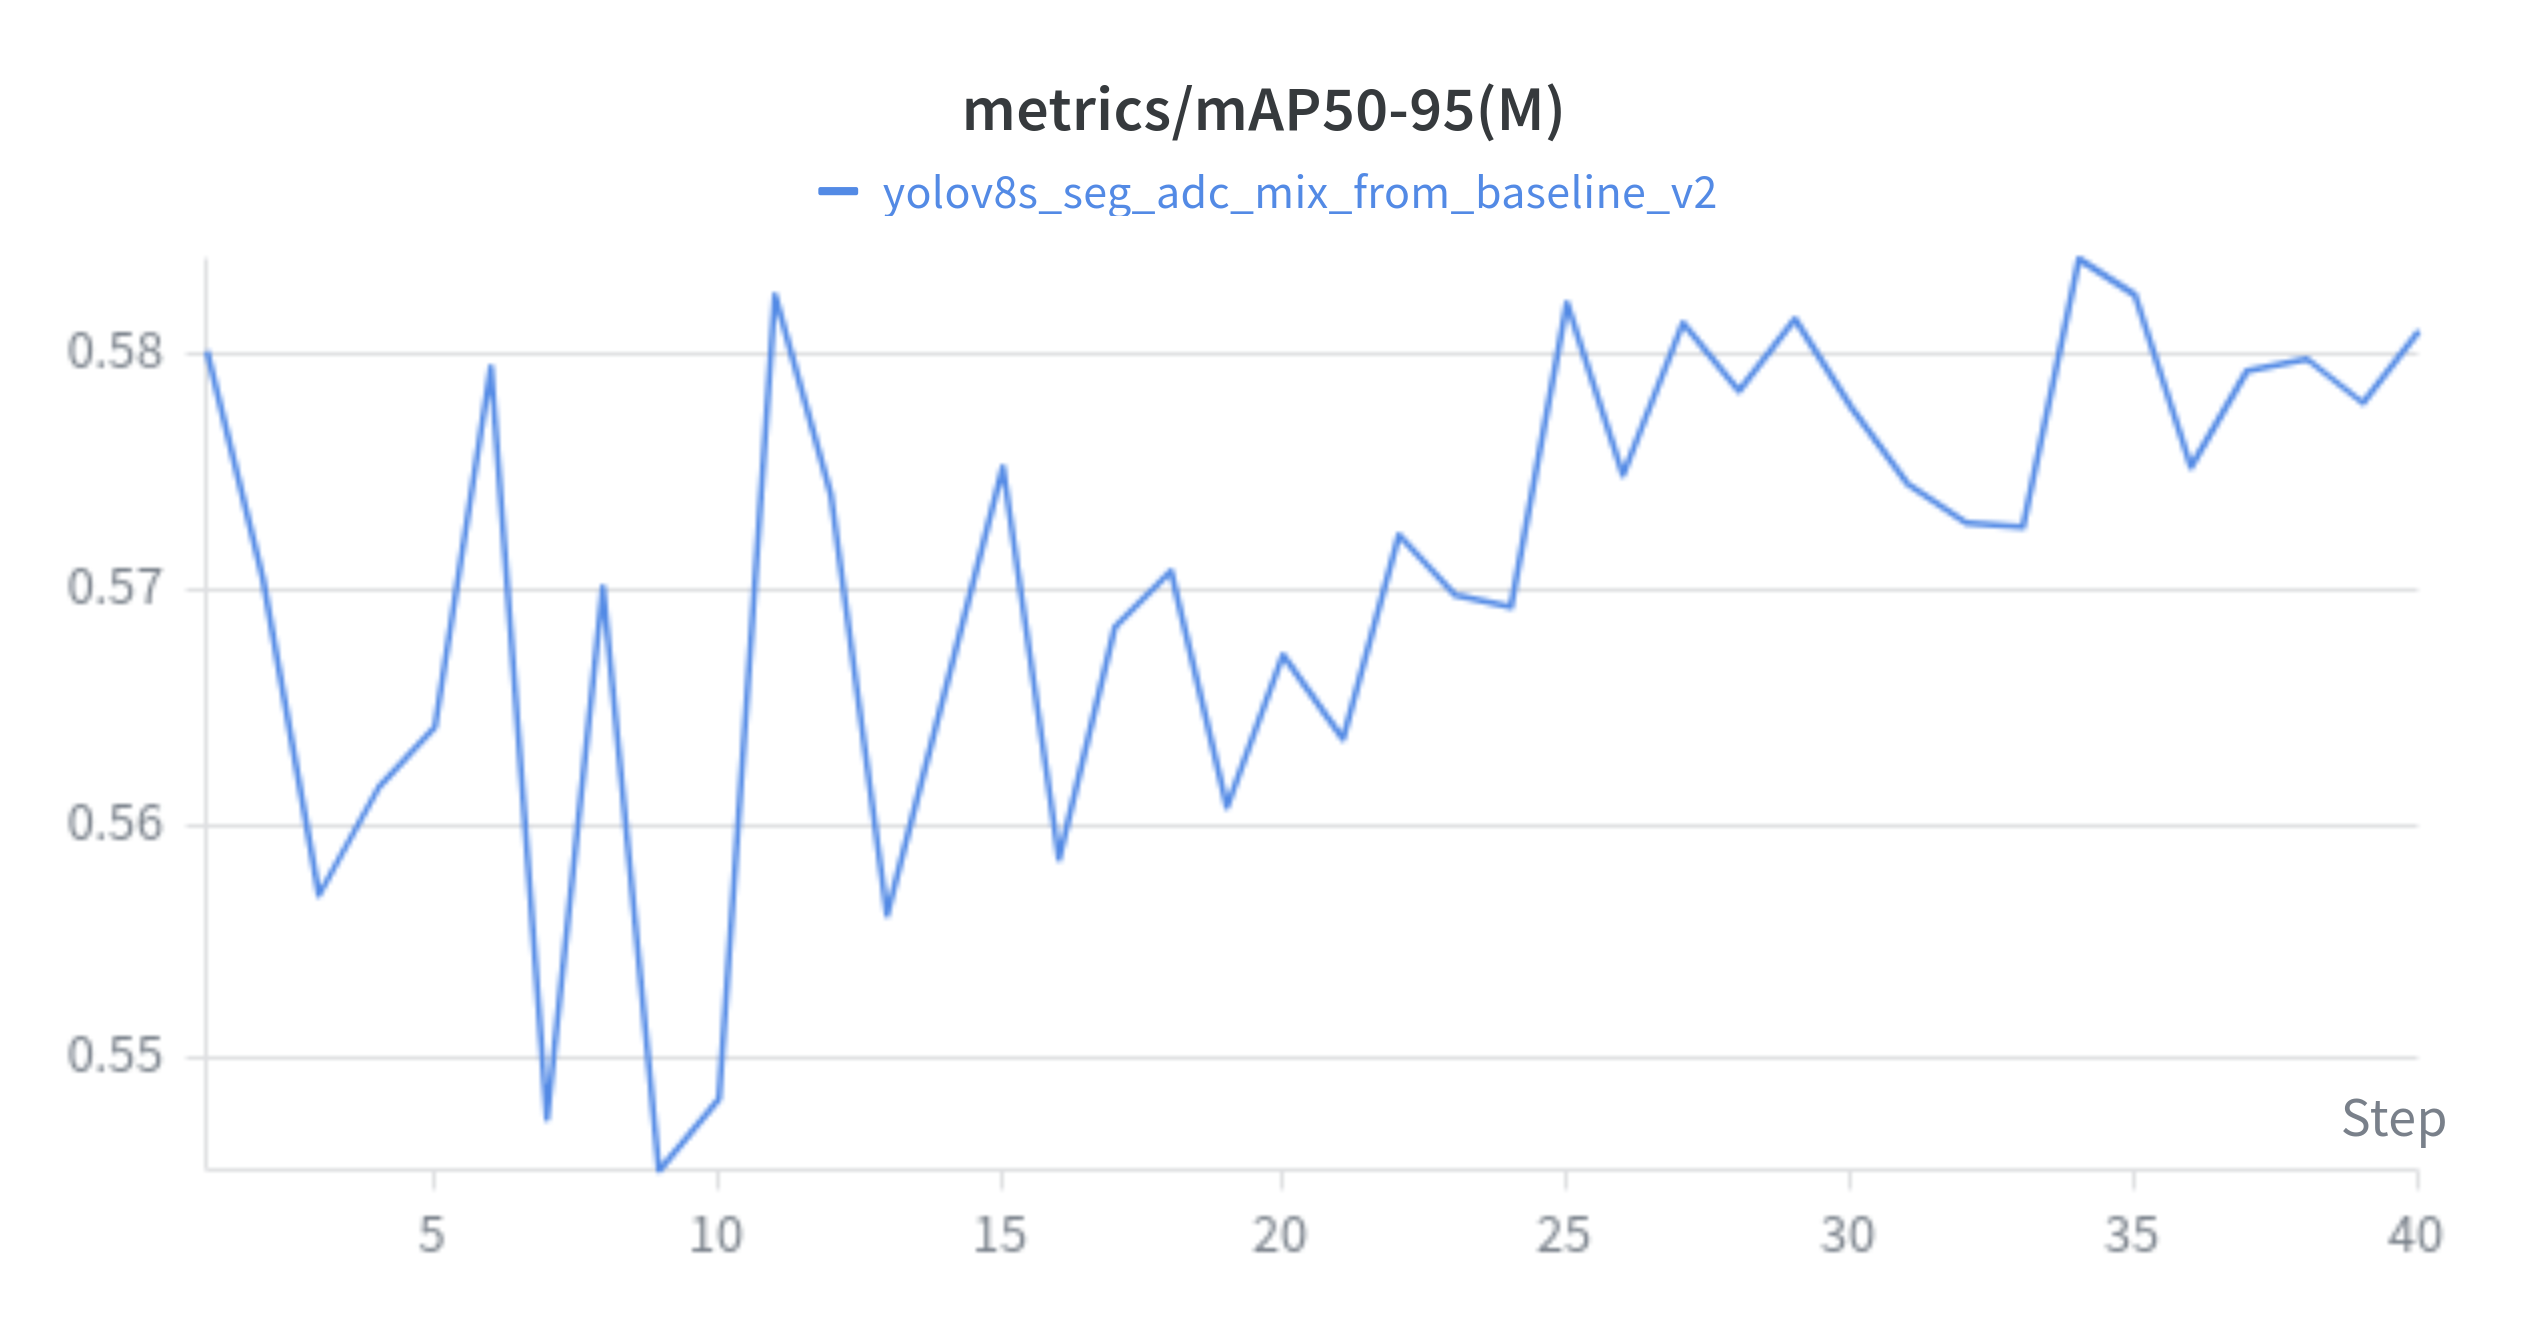
\includegraphics[width=0.82\textwidth]{figures/results/yolo_adc_fine_tune_mAP50-95_M.png}
    \caption{Validation mask $\mathrm{mAP}_{50\text{:}95}$ during \gls{adc}-based fine-tuning. The curve remains close to the baseline validation range, which aligns with the near-identical performance observed on the original held-out test split.}
    \label{fig:adc_finetune_mask_map}
\end{figure}

The effect on the \gls{adc}-specific test set is much more pronounced, as shown in
Table~\ref{tab:adc_env_test}. On this environment-specific split, the baseline
model achieved a mask $\mathrm{mAP}_{50\text{:}95}$ of only 0.12290. After
fine-tuning, the same metric increased to 0.50463. Mask precision increased from
0.61209 to 1.00000, and mask recall increased from 0.70136 to 0.99712. This is
the clearest result of the \gls{yolo} experiments: collecting a relatively small
amount of real deployment data and using it for controlled fine-tuning
substantially improved performance in the target environment while preserving the
performance level on the original test set.

\begin{table}[htbp]
    \centering
    \caption{Performance on the environment-specific \gls{adc} test split before and after \gls{adc} fine-tuning.}
    \label{tab:adc_env_test}
    \small
    \begin{tabular}{lcccc}
        \toprule
        Model & Mask $\mathrm{mAP}_{50}$ & Mask $\mathrm{mAP}_{50\text{:}95}$ & Mask precision & Mask recall \\
        \midrule
        Baseline YOLOv8-Seg & 0.53520 & 0.12290 & 0.61209 & 0.70136 \\
        \glsentryshort{adc} fine-tuned YOLOv8-Seg & 0.99500 & 0.50463 & 1.00000 & 0.99712 \\
        \bottomrule
    \end{tabular}
\end{table}

This environment-specific improvement was also reflected in deployment-oriented
behavior after retraining on \gls{adc} data from HAN University, Building 31.
In a controlled replay experiment on the same recorded \gls{rgbd} sequence, the
retrained model increased mean target confidence from 0.8184 to 0.8422 and
raised the 10th-percentile target confidence from 0.6562 to 0.7727, indicating
that the main gain occurred in weaker detections rather than only in already
easy cases. Distance-related improvements were more scenario-dependent, but live
deployment observations showed a practical increase in outside elevator-panel
single-button recognition distance from approximately 35~cm to 75~cm. This
distance gain should be interpreted as a task-specific field observation rather
than a universal range increase across all scenes, but it still supports the
conclusion that retraining improved practical usability in the target building.

Overall, the \gls{yolo} results show three main findings. First, the baseline
\gls{yolo}v8-Seg model was already strong and difficult to surpass on the general
elevator test set. Second, staged hyperparameter tuning improved validation
performance but did not fundamentally change the final model ranking. Third, the
most practically valuable improvement was achieved through environment-specific
fine-tuning with \gls{adc} data, which substantially increased performance on the
target deployment domain while preserving performance on the original dataset.

\section{\Gls{ocr} hyperparameter tuning and evaluation}

The \gls{ocr} experiments focused on improving cropped-button recognition while keeping
the recognizer lightweight enough for later embedded deployment. As in the
\gls{yolo} experiments, model selection during \gls{ocr} tuning was based on the
validation split, and the final comparison between \gls{ocr} candidates was performed on
the held-out \gls{ocr} test set.

\subsection{Stage 1: epoch selection}

The first \gls{ocr} tuning stage varied only the number of training epochs while keeping
the optimizer configuration fixed. The main objective of this stage was to
determine whether the original 60-epoch fine-tuning recipe was necessary or
whether a shorter training budget would already achieve the same validation
quality.

Table~\ref{tab:ocr_stage1_results} shows that the 50-epoch and 60-epoch runs
converged to almost identical validation performance, both reaching their best
result at epoch 46. In contrast, the 30-epoch run underperformed clearly. This
indicates that the recognizer required more than 30 epochs to converge, but that
training beyond 50 epochs provided no meaningful additional benefit. For that
reason, 50 epochs were selected as the fixed budget for the next stage of \gls{ocr}
hyperparameter tuning. This interpretation is also supported by the Stage 1
training-loss curves shown in Figure~\ref{fig:ocr_stage1_loss}, where the main
decrease occurs well before the end of the 50-epoch run and the longer schedule
does not suggest a qualitatively different convergence regime.

\begin{figure}[htbp]
    \centering
    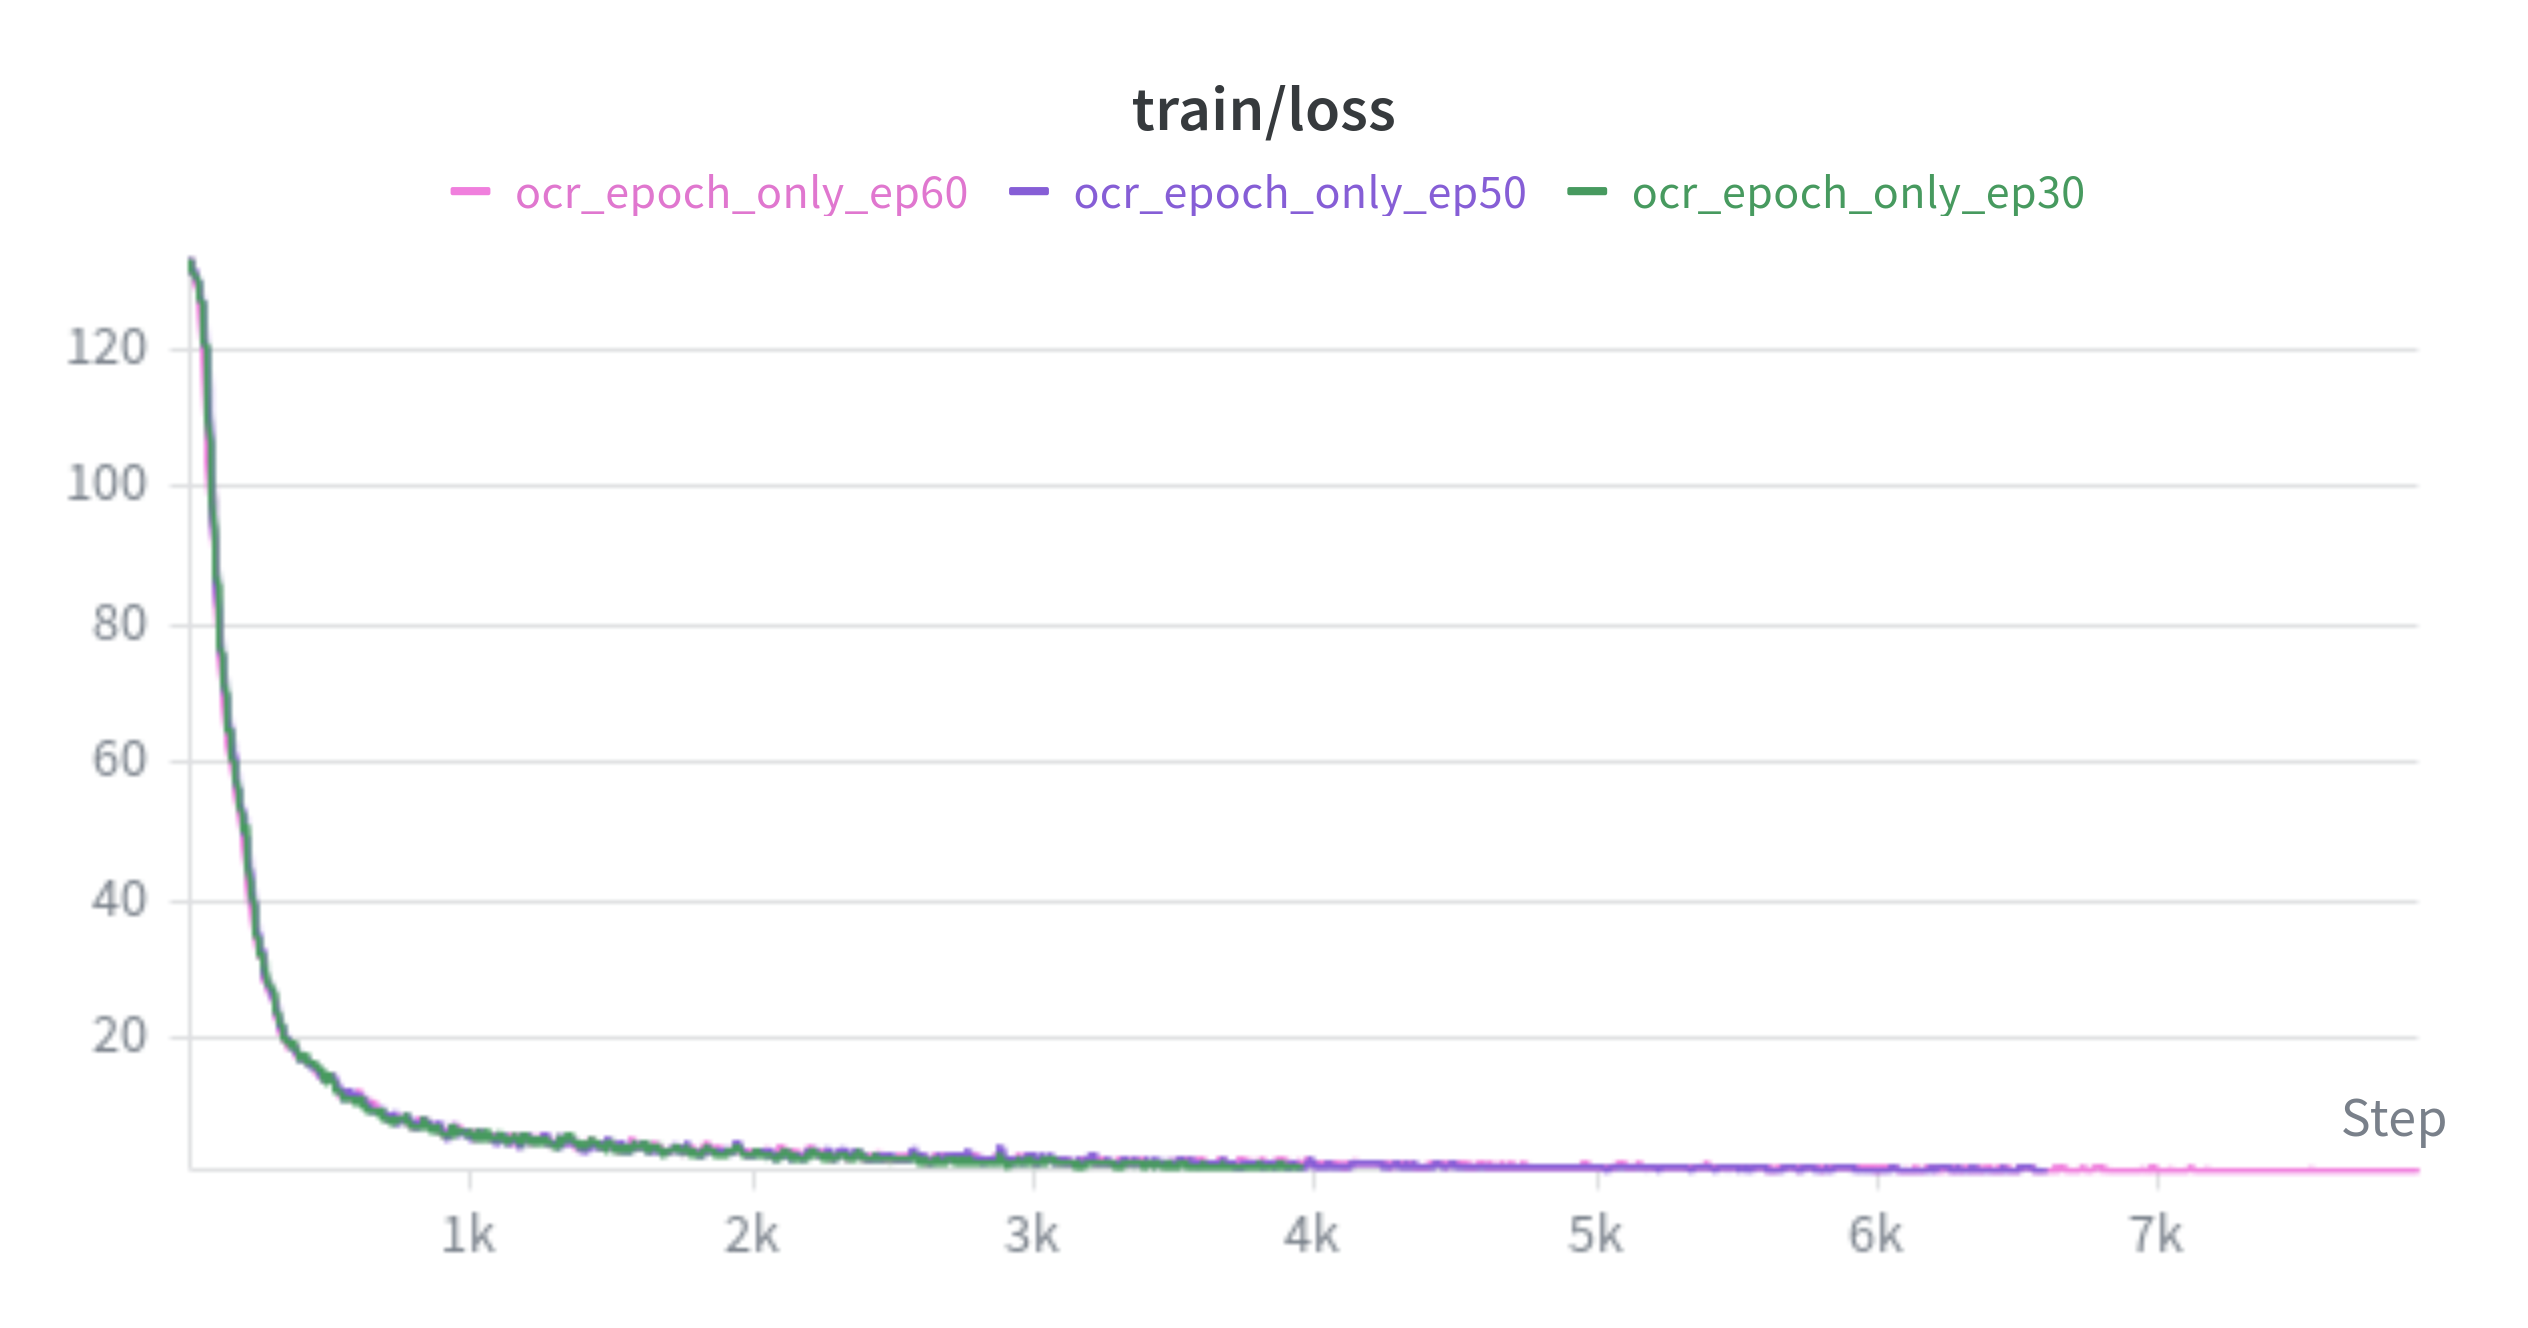
\includegraphics[width=0.82\textwidth]{figures/results/stage1_ocr_train_loss.png}
    \caption{Stage 1 \gls{ocr} training loss for the epoch-selection runs. Most of the
    optimization progress occurs before the 50-epoch mark, which supports the
    decision to use 50 epochs for the subsequent optimizer sweep.}
    \label{fig:ocr_stage1_loss}
\end{figure}

\begin{table}[htbp]
    \centering
    \caption{Stage 1 \gls{ocr} epoch-sweep results on the validation split.}
    \label{tab:ocr_stage1_results}
    \small
    \begin{tabular}{lccc}
        \toprule
        Trial & Best epoch & Accuracy & Normalized edit distance \\
        \midrule
        30 epochs & 16 & 0.78776 & 0.83732 \\
        50 epochs & 46 & 0.84124 & 0.87080 \\
        60 epochs & 46 & 0.84057 & 0.86893 \\
        \bottomrule
    \end{tabular}
\end{table}

\subsection{Stage 2: learning rate and weight decay sweep}

After fixing the training budget at 50 epochs, a second tuning stage evaluated a
narrow optimizer sweep over learning rate and weight decay. Four configurations
were tested. The resulting validation scores are summarized in
Table~\ref{tab:ocr_stage2_results}.

The best configuration used an initial learning rate of
$3 \times 10^{-4}$ and a weight decay of $3 \times 10^{-5}$. This run achieved a
validation accuracy of 0.84157 and a normalized edit distance of 0.87098, making
it the strongest \gls{ocr} candidate of the sweep. The configuration with the same
learning rate but lower weight decay performed substantially worse, while the run
using $5 \times 10^{-4}$ degraded sharply and converged to a much lower
performance level. Increasing the learning rate further to $7 \times 10^{-4}$
recovered most of the performance, but still remained below the best
$3 \times 10^{-4}$ run.

These results indicate that \gls{ocr} fine-tuning was sensitive to the optimizer
settings even within a relatively narrow search range. In particular, the stage-2
results suggest that a slightly lower learning rate than the original baseline
provided more stable and ultimately better convergence on the recognition task.
This behavior is visible in Figure~\ref{fig:ocr_stage2_acc}, where the best run
maintains the highest evaluation accuracy, and in
Figure~\ref{fig:ocr_stage2_ned}, where the same configuration also produces the
strongest normalized edit-distance curve.

\begin{figure}[htbp]
    \centering
    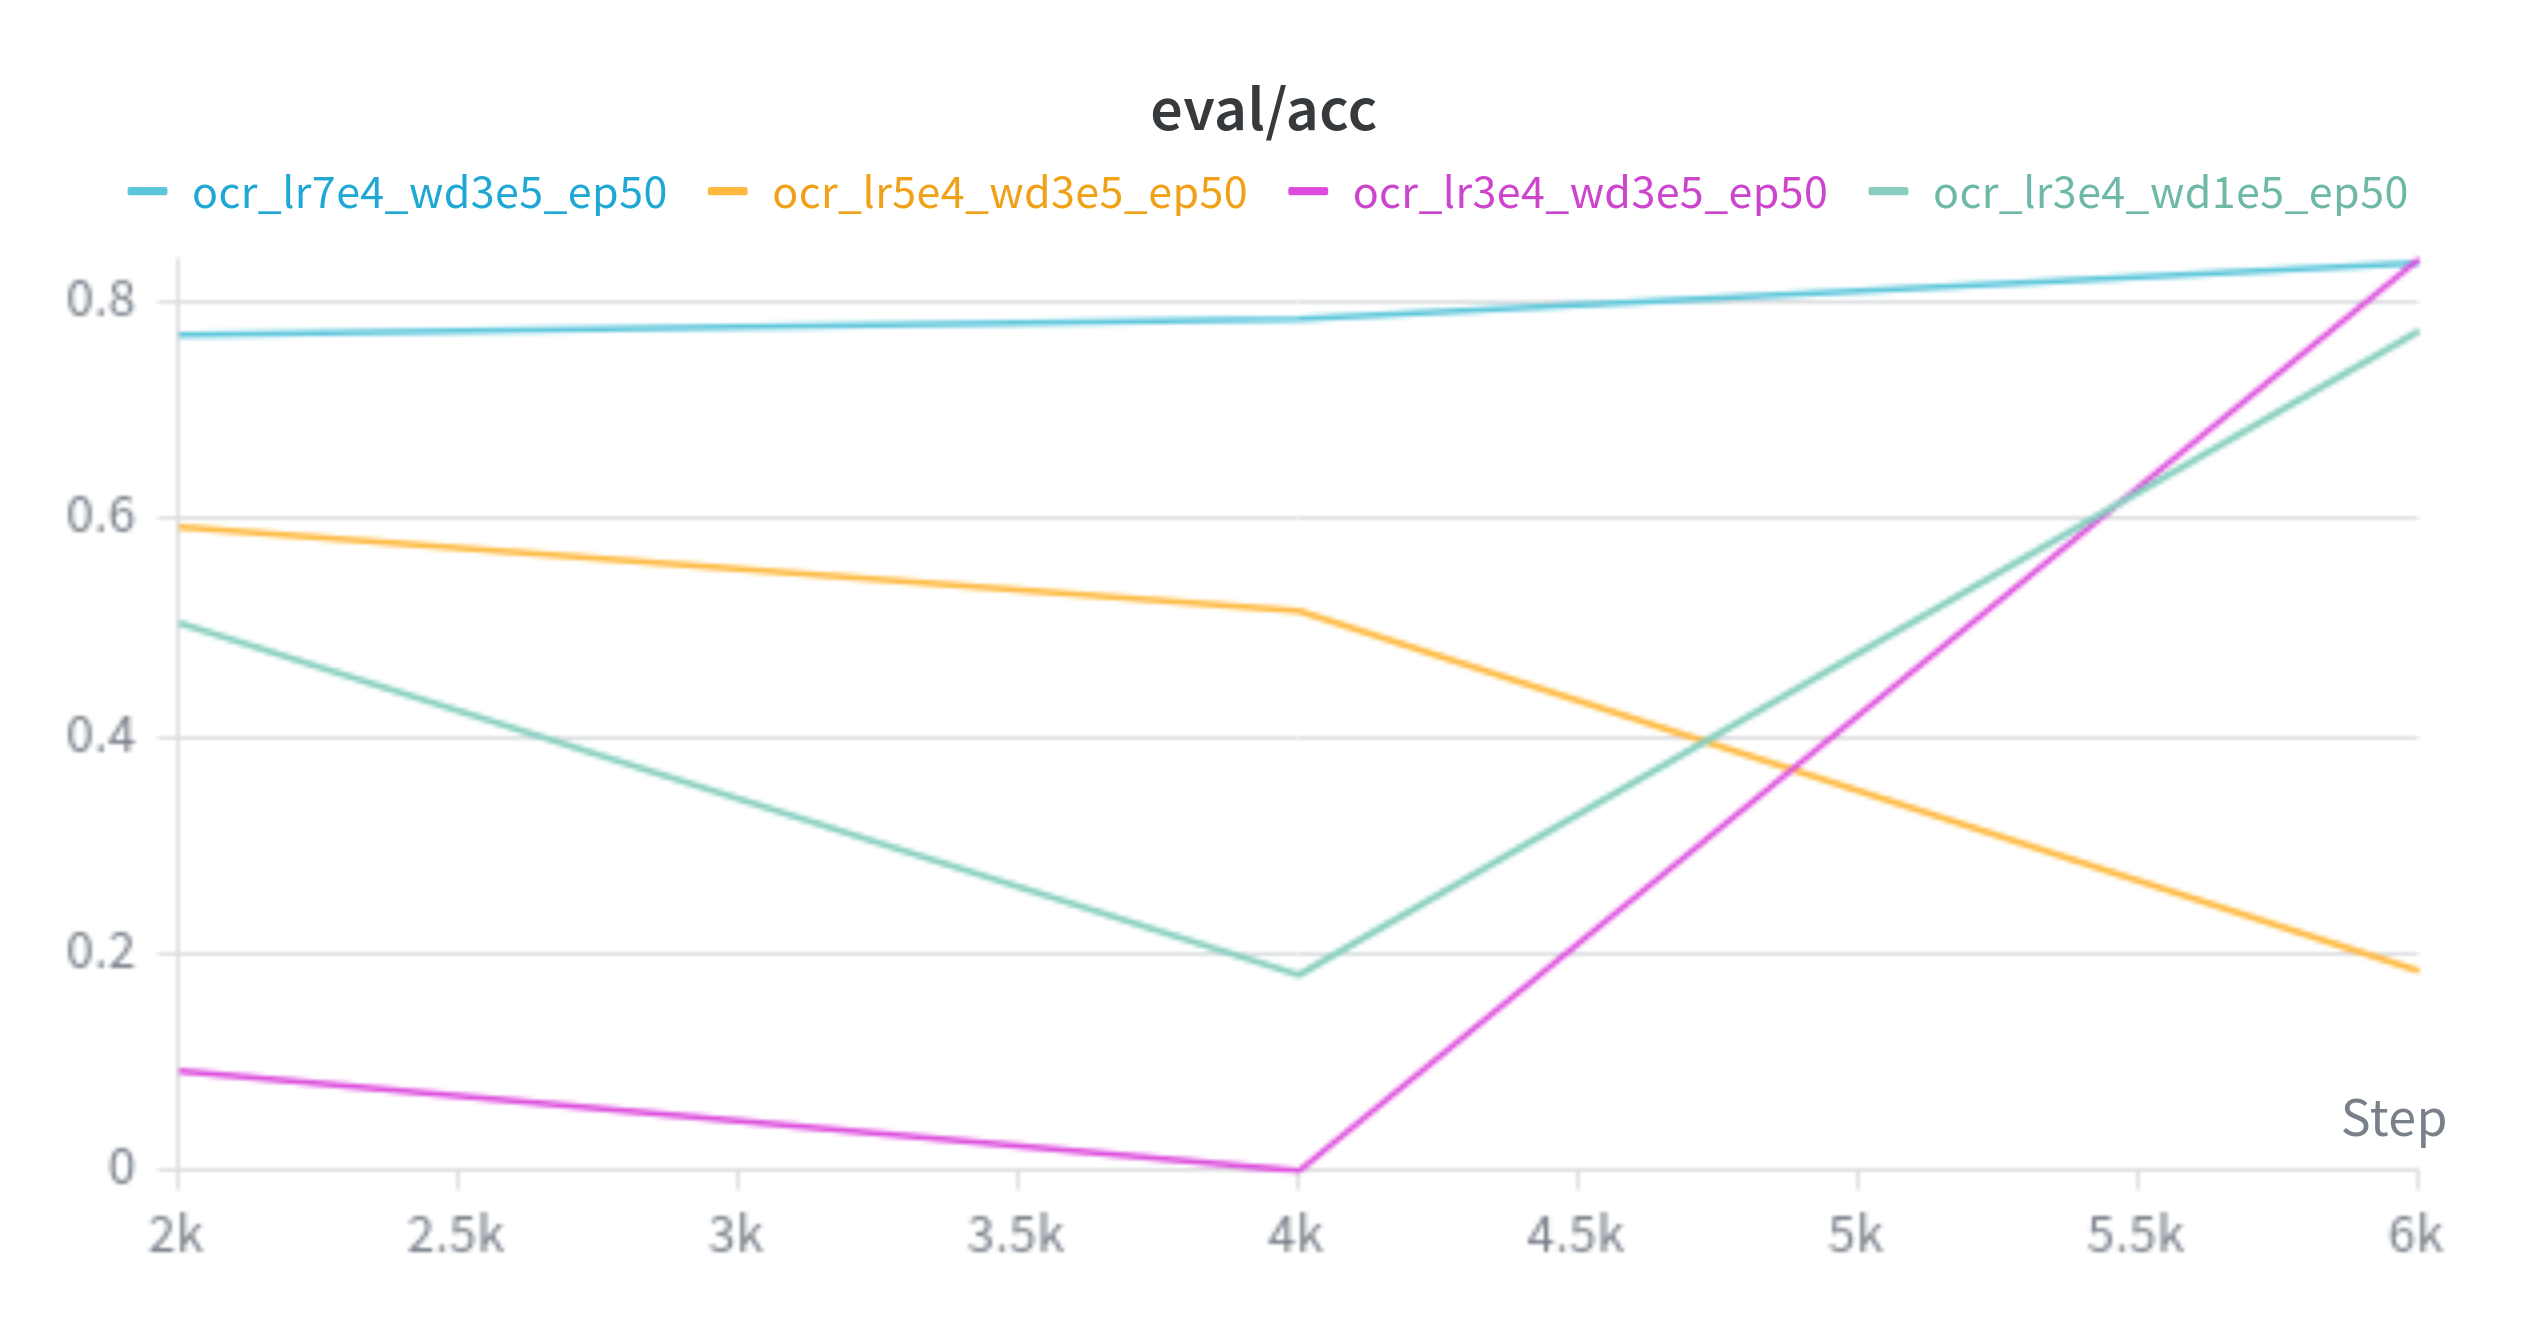
\includegraphics[width=0.82\textwidth]{figures/results/stage2_ocr_eval_acc.png}
    \caption{Stage 2 \gls{ocr} evaluation accuracy for the learning-rate and
    weight-decay sweep. The configuration with learning rate
    $3 \times 10^{-4}$ and weight decay $3 \times 10^{-5}$ achieved the best
    validation accuracy.}
    \label{fig:ocr_stage2_acc}
\end{figure}

\begin{figure}[htbp]
    \centering
    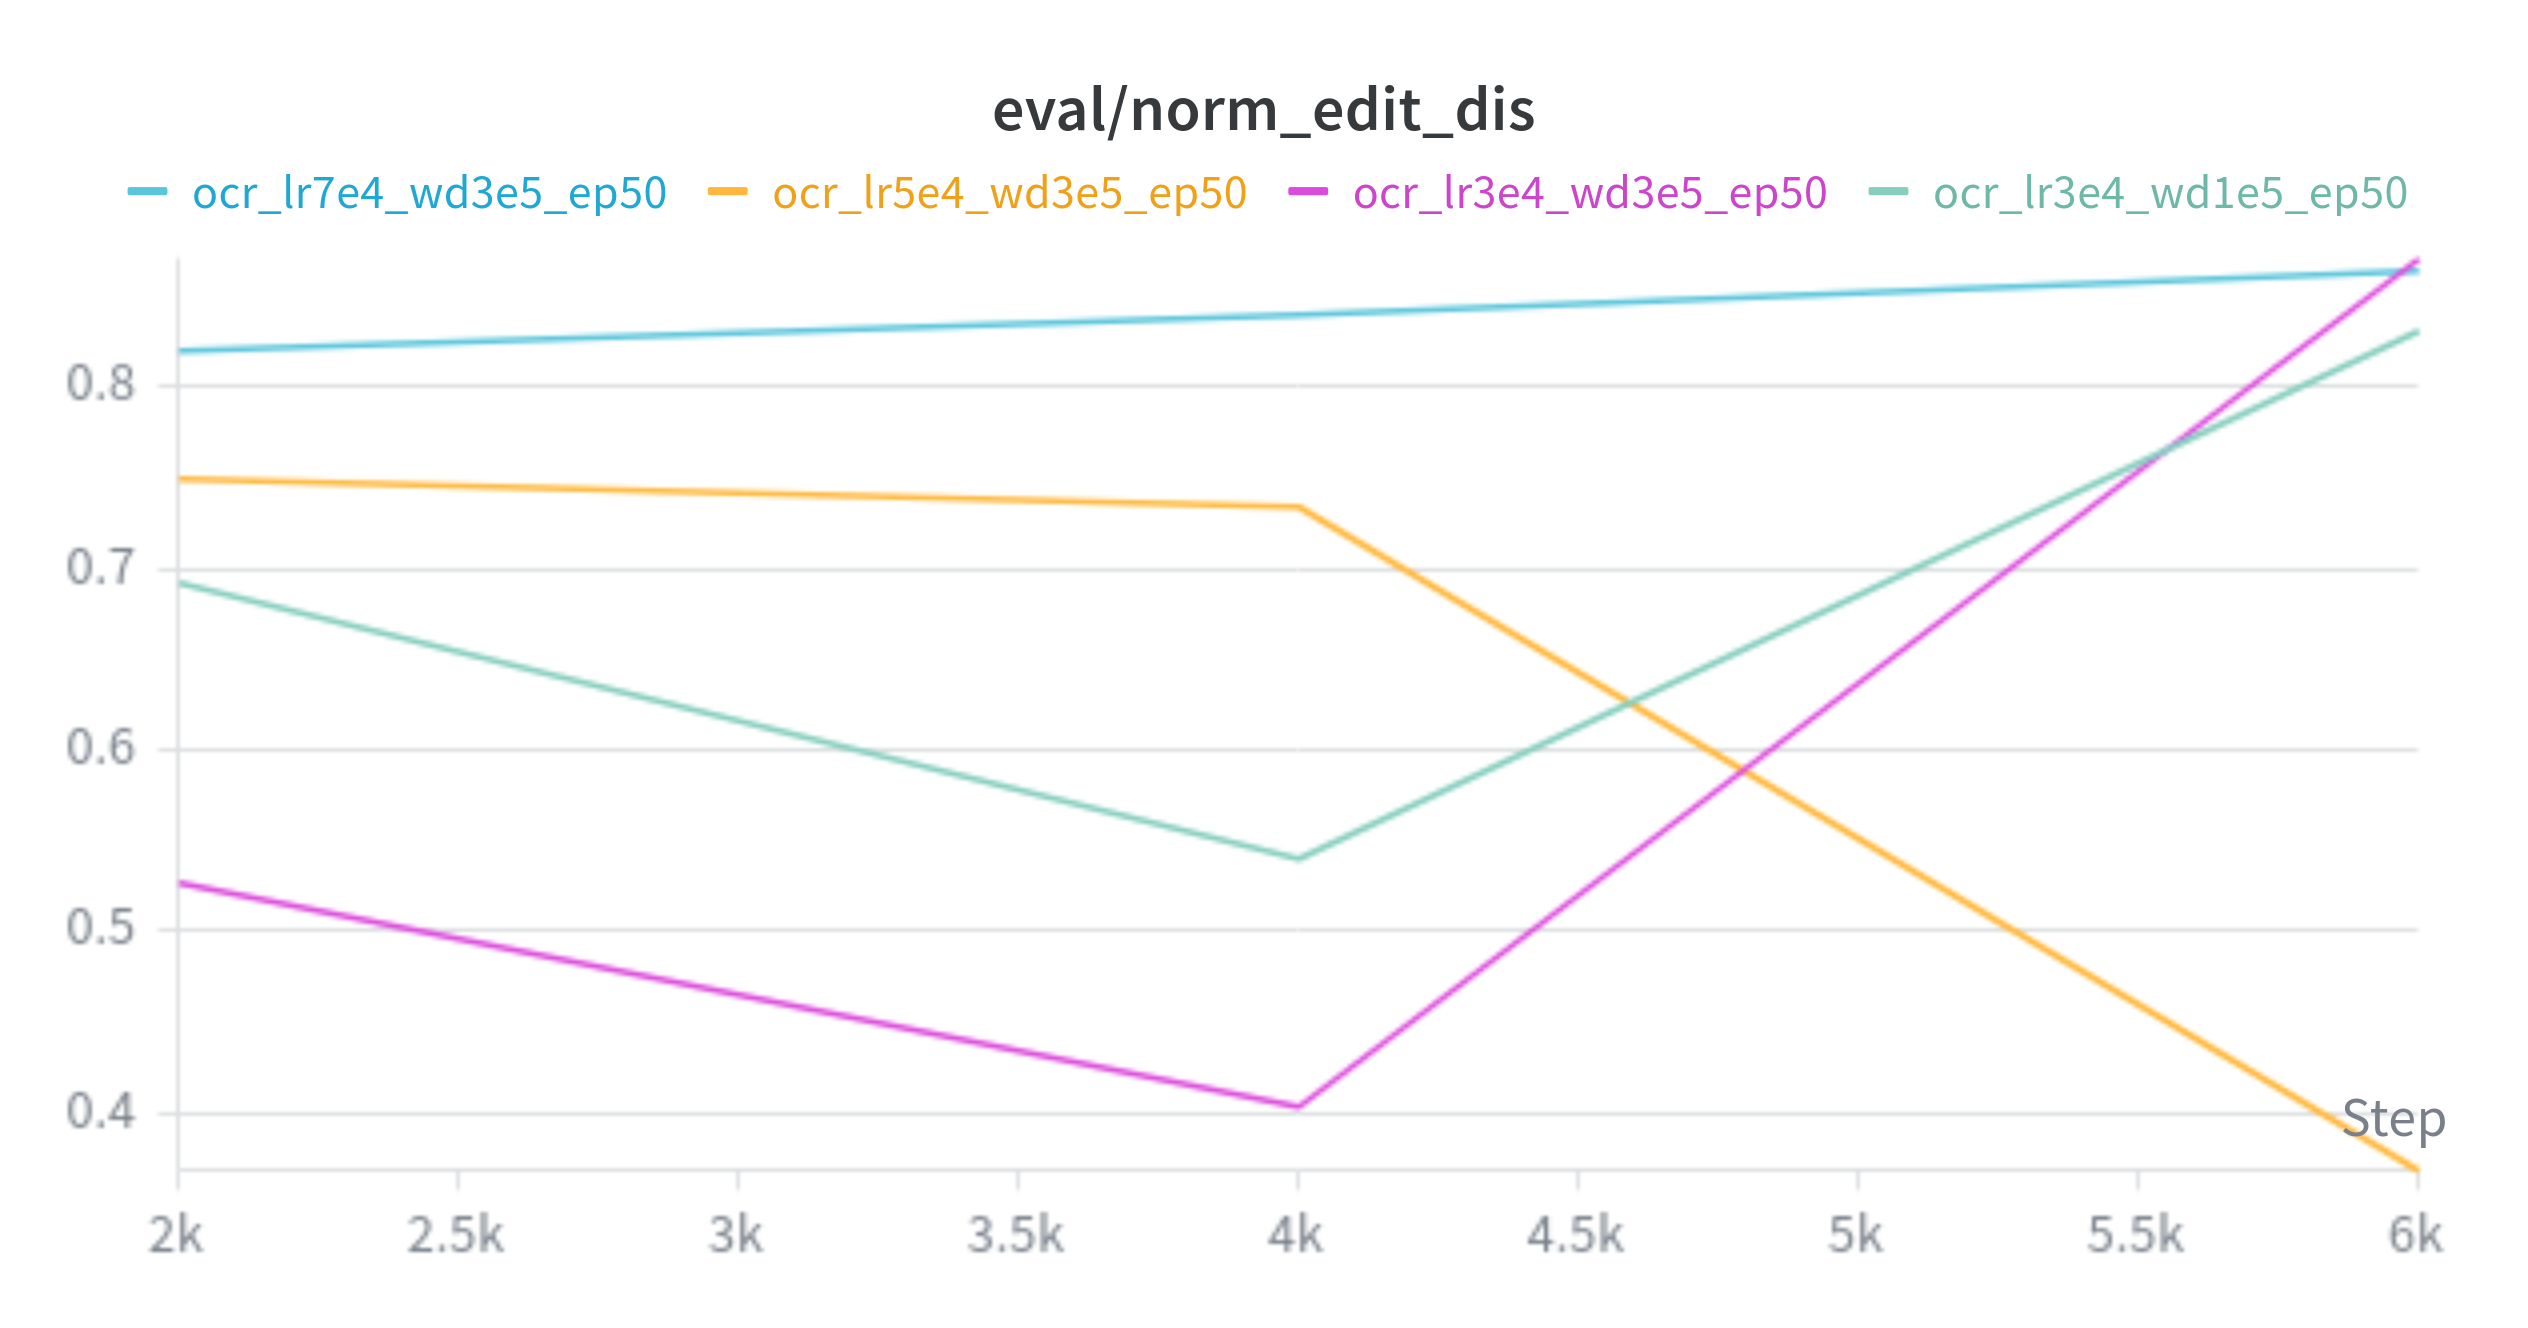
\includegraphics[width=0.82\textwidth]{figures/results/stage2_ocr_eval_norm_edit_dis.png}
    \caption{Stage 2 \gls{ocr} normalized edit distance for the learning-rate and
    weight-decay sweep. The best-performing configuration also achieved the
    highest normalized edit-distance score.}
    \label{fig:ocr_stage2_ned}
\end{figure}

\begin{table}[htbp]
    \centering
    \caption{Stage 2 \gls{ocr} hyperparameter sweep on the validation split.}
    \label{tab:ocr_stage2_results}
    \small
    \begin{tabular}{lcccc}
        \toprule
        Trial & Learning rate & Weight decay & Accuracy & Normalized edit distance \\
        \midrule
        lr3e4\_wd1e5\_ep50 & $3 \times 10^{-4}$ & $1 \times 10^{-5}$ & 0.77531 & 0.83148 \\
        lr3e4\_wd3e5\_ep50 & $3 \times 10^{-4}$ & $3 \times 10^{-5}$ & \textbf{0.84157} & \textbf{0.87098} \\
        lr5e4\_wd3e5\_ep50 & $5 \times 10^{-4}$ & $3 \times 10^{-5}$ & 0.59603 & 0.74899 \\
        lr7e4\_wd3e5\_ep50 & $7 \times 10^{-4}$ & $3 \times 10^{-5}$ & 0.83653 & 0.86546 \\
        \bottomrule
    \end{tabular}
\end{table}

\subsection{Final \gls{ocr} benchmark}

The final \gls{ocr} benchmark compared the original fine-tuned recognizer against the
best-performing stage-2 configuration on the held-out \gls{ocr} test set. The results
are shown in Table~\ref{tab:ocr_final_benchmark}. The stage-2 model outperformed
the initial \gls{ocr} model on both recognition-quality metrics. Test accuracy improved
from 0.81635 to 0.83486, while normalized edit distance improved from 0.85574 to
0.87190. In addition, the measured evaluation throughput increased slightly from
805.68 to 817.71 samples per second.

Taken together, these results show that the \gls{ocr} hyperparameter tuning process
produced a real improvement rather than only a validation-specific gain. Unlike
the \gls{yolo} tuning experiments, where better validation performance did not
translate into a better final test-set model, the \gls{ocr} stage-2 winner also
improved the held-out test benchmark. For this reason, the stage-2 best \gls{ocr} model
was selected as the final recognition candidate for later integration into the
complete perception pipeline.

\begin{table}[htbp]
    \centering
    \caption{Held-out \gls{ocr} test-set comparison between the initial recognizer and the selected stage-2 \gls{ocr} model.}
    \label{tab:ocr_final_benchmark}
    \small
    \begin{tabular}{lccc}
        \toprule
        Model & Accuracy & Normalized edit distance & Throughput (samples/s) \\
        \midrule
        Initial \glsentryshort{ocr} model & 0.81635 & 0.85574 & 805.68 \\
        Stage-2 best \glsentryshort{ocr} model & \textbf{0.83486} & \textbf{0.87190} & \textbf{817.71} \\
        \bottomrule
    \end{tabular}
\end{table}

\subsection{Model hardware optimization results}

As described in Chapter~3, the final \gls{yolo} and \gls{ocr} models were
exported to \gls{tensorrt} for optimized execution on the \gls{jetson} platform.
To verify the effect of this export step, a compact benchmark was performed on
the held-out test image \texttt{367.jpg}. For \gls{yolo}, the comparison used the
PyTorch checkpoint and the exported \gls{tensorrt} engine on the same full image.
For \gls{ocr}, the comparison used the Paddle inference model and the exported
\gls{tensorrt} engine on the five annotated button crops from the same image.

\begin{table}[htbp]
    \centering
    \caption{Single-image model hardware optimization benchmark on test image \texttt{367.jpg}. For \gls{ocr}, the reported latency is average time per single button crop.}
    \label{tab:model_hw_optimization}
    \small
    \begin{tabular}{lccc}
        \toprule
        Model stage & Baseline backend & \glsentryshort{tensorrt} backend & Speedup \\
        \midrule
        \glsentryshort{yolo} inference [ms/image] & 36.46 & 24.43 & 1.49$\times$ \\
        \glsentryshort{yolo} wall time [ms/image] & 64.19 & 64.52 & 1.00$\times$ \\
        \glsentryshort{ocr} latency [ms/crop] & 167.72 & 10.29 & 16.30$\times$ \\
        \bottomrule
    \end{tabular}
\end{table}

The \gls{yolo} result shows that \gls{tensorrt} reduced the forward-pass time
substantially, even though the total offline single-image wall time remained
almost unchanged because preprocessing and postprocessing still contributed a
large fraction of the runtime. The \gls{ocr} result is more direct: the
\gls{tensorrt} engine reduced average latency from 167.72~ms to 10.29~ms per
button crop while preserving the same accepted predictions on all five button
regions in the test image. These results support the use of \gls{tensorrt}
export as an important deployment optimization step before integrating the models
into the full \gls{ros2} pipeline.

\section{\Gls{ros2} pipeline performance}

After the final \gls{yolo} and \gls{ocr} models were exported to \gls{tensorrt}, the complete
perception stack was evaluated on the \gls{jetson} Orin Nano in its deployed \gls{ros2}
configuration. The purpose of these experiments was not to compare neural-network
accuracy, but to quantify the practical throughput of the integrated pipeline under
different runtime settings. The reported measurements correspond to the final
post-refactor pipeline in which ROI-local masks are published by the YOLO node and
full-image annotation reconstruction is performed only inside the \gls{adc} when
export is required. During these experiments, the Stereolabs ZED X camera was
launched with the \texttt{zedx} wrapper profile, which uses a native
\texttt{HD1200} grab mode at 30~Hz and publishes rectified color and depth data at
15~\gls{fps}. With the configured downscale factor of 2.0, the effective published
image resolution used by the perception pipeline was 960$\times$600 pixels.

Three final runtime scenarios were compared:
\begin{itemize}
    \item camera + \gls{yolo} + \gls{ocr} + \gls{adc},
    \item camera + \gls{yolo} + \gls{ocr} without collector and with \gls{ocr} uncapped, and
    \item camera + \gls{yolo} + \gls{ocr} without collector and with \gls{ocr} limited to four regions per message.
\end{itemize}

Table~\ref{tab:ros2_pipeline_fps} summarizes the resulting topic throughput. The
collector-enabled configuration sustained approximately 10~\gls{fps} while preserving
the full deployment data-collection path. When the collector was disabled and \gls{ocr}
was allowed to process all candidate regions, the end-to-end rate increased to
about 12.2~\gls{fps}. The best runtime-oriented configuration was obtained when \gls{ocr}
was capped to four regions per message, yielding approximately 13.1~\gls{fps}
end-to-end on the final \texttt{/button\_targets\_3d\_ocr} output topic. The
reported topic rates were measured with the standard \texttt{ros2 topic hz}
utility on the relevant output topics.

\begin{table}[htbp]
    \centering
    \caption{Final \gls{ros2} pipeline throughput on the \gls{jetson} Orin Nano after the ROI-mask refactor, measured with \texttt{ros2 topic hz}.}
    \label{tab:ros2_pipeline_fps}
    \small
    \begin{tabular}{lcc}
        \toprule
        Configuration & \texttt{/button\_targets\_3d} \gls{fps} & \texttt{/button\_targets\_3d\_ocr} \gls{fps} \\
        \midrule
        With collector & $\sim 10.0$ & $\sim 10.0$ \\
        No collector, \gls{ocr} uncapped & $\sim 12.15$ & $\sim 12.29$ \\
        No collector, \gls{ocr} capped to 4 ROIs & $\sim 13.14$--$13.47$ & $\sim 13.08$--$13.25$ \\
        \bottomrule
    \end{tabular}
\end{table}

The timing breakdown confirms that the final system bottleneck is not the \gls{tensorrt}
forward pass alone, but the combined cost of segmentation postprocessing, depth
estimation, and \gls{ocr} execution inside the live \gls{ros2} graph. Table~\ref{tab:ros2_pipeline_timing}
shows typical timing ranges of the \gls{yolo} and \gls{ocr} nodes for the three runtime
configurations. In collector mode, the YOLO node required approximately
81--91~ms per callback and the \gls{ocr} node 79--95~ms. Removing the collector while
keeping \gls{ocr} uncapped reduced the practical throughput penalty of data export but
still required roughly 11 processed \gls{ocr} regions per message, which kept \gls{ocr} total
time in the 77--102~ms range. Limiting \gls{ocr} to four regions reduced \gls{ocr} total time
to roughly 33--35~ms and allowed the complete pipeline to reach its best measured
throughput.

\begin{table}[htbp]
    \centering
    \caption{Typical node timing ranges for the final \gls{ros2} runtime experiments.}
    \label{tab:ros2_pipeline_timing}
    \small
    \resizebox{\textwidth}{!}{%
    \begin{tabular}{lcccc}
        \toprule
        Configuration & \glsentryshort{yolo} total [ms] & \glsentryshort{yolo} depth [ms] & \glsentryshort{ocr} total [ms] & \glsentryshort{ocr} processed ROIs \\
        \midrule
        With collector & $\sim 81$--$91$ & $\sim 3.6$--$6.6$ & $\sim 79$--$95$ & not capped \\
        No collector, \gls{ocr} uncapped & $\sim 78$--$99$ & $\sim 4$--$7$ & $\sim 77$--$102$ & $\sim 10.7$--$10.9$ \\
        No collector, \gls{ocr} capped to 4 ROIs & $\sim 70.4$--$77.8$ & $\sim 5.3$--$7.0$ & $\sim 33.0$--$35.2$ & $4.0$ \\
        \bottomrule
    \end{tabular}
    }
\end{table}

These results show that the integrated perception pipeline can operate at
deployment-relevant frame rates on the \gls{jetson} Orin Nano, provided that annotation
serialization is kept out of the real-time \gls{yolo} path and \gls{ocr} workload is bounded.
For runtime operation, the most effective configuration is the ROI-limited \gls{ocr}
setup without concurrent collection, which achieved approximately 13.1~\gls{fps}.
For deployment sessions that must simultaneously gather new training data, the
collector-enabled configuration remains practical at approximately 10~\gls{fps},
which is sufficient to preserve the full adaptive data-collection loop described in
Chapter~\ref{ch:methodology}.

\chapter{Discussion}
\label{ch:discussion}

This chapter interprets the results presented in Chapter~4 and relates them to
the project objective of developing an efficient and scalable computer-vision
workflow for robot interaction with elevator infrastructure on embedded
hardware.

\section{Interpretation of the main findings}

The main outcome of this project is that a practical embedded perception
workflow can be achieved by combining instance-segmentation-based button
detection, crop-based \gls{ocr}, and a modular \gls{ros2} runtime pipeline. The
results show that the strongest overall system did not come from selecting the
newest model architecture or from maximizing validation performance in isolation.
Instead, the most effective workflow emerged from a sequence of engineering
decisions that balanced perception quality, deployment constraints, and future
scalability.

For \gls{yolo}, the baseline \gls{yolo}v8-Seg model remained the most reliable
choice for deployment. Hyperparameter tuning improved validation performance, but
those gains did not translate into a better final held-out test model. Likewise,
YOLO26-small did not outperform the baseline under the same evaluation
conditions. This is an important result because it shows that, for this task, a
carefully chosen and well-understood baseline can be more valuable than adopting
a newer architecture without a clear deployment benefit. The most practically
useful \gls{yolo} improvement came from environment-specific fine-tuning with
\gls{adc} data from HAN University, Building 31, which substantially improved
performance in the target environment while preserving the original-domain
performance.

For \gls{ocr}, the project produced a clearer tuning outcome. The selected stage-2
configuration improved both test accuracy and normalized edit distance relative
to the initial recognizer. In contrast to the \gls{yolo} tuning results, the
\gls{ocr} validation improvements did translate into better held-out test-set
performance. This suggests that the \gls{ocr} stage was more sensitive to
optimization settings in a way that remained meaningful at test time.

At system level, the deployed \gls{ros2} pipeline demonstrates that model
quality alone is not sufficient for real-time embedded performance. The final
pipeline throughput depended strongly on how much non-inference work remained in
the runtime path. The shift from full-image mask export to compact ROI-local mask
handling, together with the split-node \gls{yolo}/\gls{ocr} architecture and the
bounded \gls{ocr} workload, produced the most important runtime gains. The best
measured configuration achieved about 13.1~\gls{fps}, while the collector-enabled
configuration remained practical at about 10~\gls{fps}. This shows that the
embedded performance target was not reached by model export alone, but by a
combination of model export, message-design decisions, and workload placement.

\section{Relation to the research questions}

The results provide a coherent answer to the main research question. An
efficient and scalable computer-vision workflow for hospital interaction-point
perception can be designed by using instance segmentation for button localization,
crop-based \gls{ocr} for semantic interpretation, \gls{tensorrt} export for
embedded execution, and an \gls{ros2}-based split-node architecture for modular
runtime integration.

The first sub-question concerned the relevant human-interaction points in
hospital environments. The project focused on elevator buttons and related panel
interfaces because they are a concrete and operationally critical interaction
class for multi-floor service-robot mobility. This focus proved appropriate: the
task is sufficiently challenging to expose problems of detection, segmentation,
recognition, and embedded deployment, while still being narrow enough to support
a complete workflow.

The second sub-question asked which methods and architectures were suitable.
The literature review suggested that instance segmentation is better aligned with
precise robot interaction than coarse object detection alone, and the results
support this choice. The segmentation masks were directly useful for masked depth
estimation and 3D target generation. The final architecture therefore combined a
segmentation-based detector with a separate recognizer rather than relying on a
single end-to-end model.

The third sub-question concerned dataset design. The results show that dataset
quality and dataset relevance were both important. The original curated dataset
was sufficient to train a strong baseline, but the environment-specific
fine-tuning experiment demonstrated that even a relatively small amount of
deployment-collected data can substantially improve performance in the target
domain. This supports the decision to include an \gls{adc} in the full workflow.

The fourth sub-question asked which optimization techniques support embedded
inference. Here the answer is twofold. First, \gls{tensorrt} export was
beneficial for both \gls{yolo} and \gls{ocr}, with especially strong gains for
\gls{ocr}. Second, export alone was not enough: runtime-side optimizations such
as reducing annotation overhead, separating the inference nodes, and limiting the
number of processed \gls{ocr} regions were equally important.

The fifth sub-question concerned scalability and efficient future improvement.
The final system addresses this directly through the \gls{adc}, which turns
runtime use into a source of curated retraining data. The environment-specific
\gls{yolo} improvement demonstrates that this design is not only theoretically
scalable, but also practically useful.

\section{Limitations}

Several limitations should be considered when interpreting the results. First,
the project focused on elevator-interface perception rather than the full set of
hospital interaction elements. While this was a justified and useful scope
reduction, the final conclusions should not automatically be generalized to all
door panels, access readers, or human-machine interfaces.

Second, some benchmark results remain sensitive to the evaluation setup. For
example, the single-image framework-to-\gls{tensorrt} comparison is useful for
illustrating acceleration trends, but it is not by itself a complete deployment
benchmark. Likewise, some distance-related \gls{yolo} improvements were most
clearly observed in field behavior and specific replay analyses rather than in a
single universal summary metric. For this reason, the confidence and coverage
improvements are stronger conclusions than any claim of a general doubling of
recognition range.

Third, the project was executed on a single embedded platform and camera setup.
The \gls{jetson} Orin Nano and Stereolabs ZED X are representative for the
target use case, but performance and tuning decisions may differ on other edge
devices or other sensing configurations.

Fourth, the report currently emphasizes perception and runtime integration rather
than downstream manipulation or actuation. The system produces 3D button targets
and button labels, but the full closed-loop robot interaction behavior lies
beyond the present project scope.

\section{Implications for future robot deployment}

Despite these limitations, the project has clear practical implications. The
results suggest that a service robot does not require a monolithic perception
stack to achieve useful embedded performance. A modular pipeline with explicit
message interfaces can be easier to tune, benchmark, and extend. This is
particularly important for educational and research robots such as CareBot, where
iterative development and subsystem replacement are expected.

The project also suggests that deployment data should be treated as a core part
of the system design rather than as an afterthought. The inclusion of the
\gls{adc} makes the perception workflow self-improving in a structured way: the
same runtime system used in deployment can collect higher-value examples for the
next training cycle. This closes an important loop between experimentation,
deployment, and future model improvement.

Overall, the project shows that the combination of instance segmentation,
task-specific \gls{ocr}, \gls{tensorrt} acceleration, and structured deployment
data collection provides a credible foundation for later integration into a more
complete autonomous hospital robot.

\chapter{Conclusions and recommendations}
\label{ch:conclusions}

This chapter summarizes the final conclusions of the project and translates the
main findings into concrete recommendations for future work.

\section{Conclusions}

The objective of this project was to develop and validate an efficient and
scalable computer-vision workflow that enables a service-robot platform to detect
and classify human-interaction elements in hospital environments using embedded
hardware. Based on the results presented in this report, this objective was
achieved for the targeted elevator-interaction use case.

The project demonstrates that a practical embedded perception workflow can be
constructed from four main components: a strong instance-segmentation baseline
for button localization, a crop-based \gls{ocr} stage for button interpretation,
\gls{tensorrt} export for hardware-efficient inference, and a modular \gls{ros}
pipeline that integrates detection, 3D projection, text recognition, and
deployment data collection.

The main conclusions are as follows.

\begin{enumerate}
    \item Instance segmentation is an effective method for elevator-button perception because it supports both accurate 2D localization and mask-based depth estimation for 3D target generation.
    \item The baseline \gls{yolo}v8s segmentation model was the strongest deployment candidate among the evaluated detector variants. Hyperparameter tuning improved validation performance, but not the final held-out test ranking.
    \item Environment-specific fine-tuning with \gls{adc} data from Han Building R29 produced the most practically valuable \gls{yolo} improvement, substantially increasing target-domain performance while preserving original-domain performance. In the controlled single-button R29 experiment, the adapted detector produced more frames with detections (138 vs.\ 106) and longer mean and median valid-detection distances (0.4282~m vs.\ 0.3527~m and 0.4102~m vs.\ 0.3308~m, respectively) after the initial model's manually reviewed long-range false positives were excluded from the valid-distance comparison. The corresponding confidence values were very similar, indicating that the main practical gain was more reliable target coverage rather than a large confidence increase. A separate reviewed deployment-style university run further showed a clear practical trend: accepted \gls{yolo} detection confidence decreases as distance increases, which strengthens the case for treating distance as an important reliability cue during deployment.
    \item The selected stage-2 \gls{ocr} model improved held-out recognition quality and formed a suitable semantic interpretation stage for the full pipeline.
    \item \gls{tensorrt} export was beneficial for both deployed models. The effect was moderate but clear for \gls{yolo} inference time, and very strong for \gls{ocr} per-crop wall time.
    \item The final \gls{ros} pipeline achieved practical embedded runtime performance on the \gls{jetson} Orin Nano, with the best measured configuration operating at about 13.1~\gls{fps} (approximately 76~ms/frame) and the collector-enabled configuration remaining usable at about 10~\gls{fps} (approximately 100~ms/frame).
    \item Scalability is supported not only by model architecture choices, but also by the inclusion of the \gls{adc}, which enables structured deployment-time data collection for future retraining.
\end{enumerate}

Taken together, these conclusions answer the main research question: a practical
computer-vision workflow for elevator-button perception can be achieved on
embedded hardware by combining segmentation-based detection, task-specific
recognition, deployment-oriented optimization, and iterative deployment data
collection within a modular \gls{ros} architecture.

\section{Recommendations}

The following recommendations are proposed for future work and further
development of the system.

\begin{enumerate}
    \item Extend the perception scope beyond elevator buttons to additional hospital interaction elements such as access readers, door controls, and other panel interfaces.
    \item Perform larger and more controlled deployment trials in multiple buildings so that domain shift, lighting variation, and panel diversity can be evaluated more systematically.
    \item Continue using the \gls{adc} as part of regular deployment, with periodic review, further fine-tuning, and retraining cycles based on newly collected field samples.
    \item Strengthen the hyperparameter tuning process for both the \gls{yolo} and \gls{ocr} models by using broader and more systematic searches, so that future model updates are based on more stable and better-validated configurations.
    \item Automate the improvement cycle further by reducing manual steps between \gls{adc} export, annotation verification, training, and redeployment, so that future model updates require less manual coordination.
    \item Perform real robot trials in hospital-like and, when possible, actual hospital environments so that the perception pipeline can be validated under realistic operational constraints and new deployment data can be collected systematically.
    \item Replace the current Jetson microSD-based storage setup with an SSD-based configuration to improve robustness for logging, dataset export, and long deployment sessions.
    \item Reimplement runtime-critical \gls{ros} nodes in C++ where appropriate, since the current Python implementation is practical for development but likely leaves performance headroom on the embedded platform.
    \item Evaluate the pipeline on additional embedded platforms to determine how transferable the optimization choices are beyond the current \gls{jetson}-based setup.
    \item Integrate the perception pipeline with downstream robot action modules so that the 3D target estimates can be validated in full interaction tasks rather than perception-only experiments.
\end{enumerate}

\section{Final reflection}

This project provides a concrete foundation for autonomous interaction with
elevator infrastructure in hospital-like environments. More broadly, it shows
that robust embedded perception is not achieved by model selection alone. The
best results emerged from treating dataset design, model choice, runtime
architecture, and deployment data collection as one connected system. That
systems perspective is likely to remain essential as the CareBOTS platform evolves
toward more complete autonomous operation in real healthcare environments.


% ---------- References ----------
\clearpage
\bibliography{references}

% ---------- Appendices ----------
\appendix
\chapter{Supplementary hyperparameter tuning curves}
\label{app:hparam_tuning}

\section{YOLO hyperparameter tuning curves}
\label{app:yolo_hparam_curves}

This appendix collects supporting \gls{yolo} hyperparameter-tuning figures that
were removed from the main results chapter to keep the core model-selection
narrative concise.

\begin{figure}[H]
    \centering
    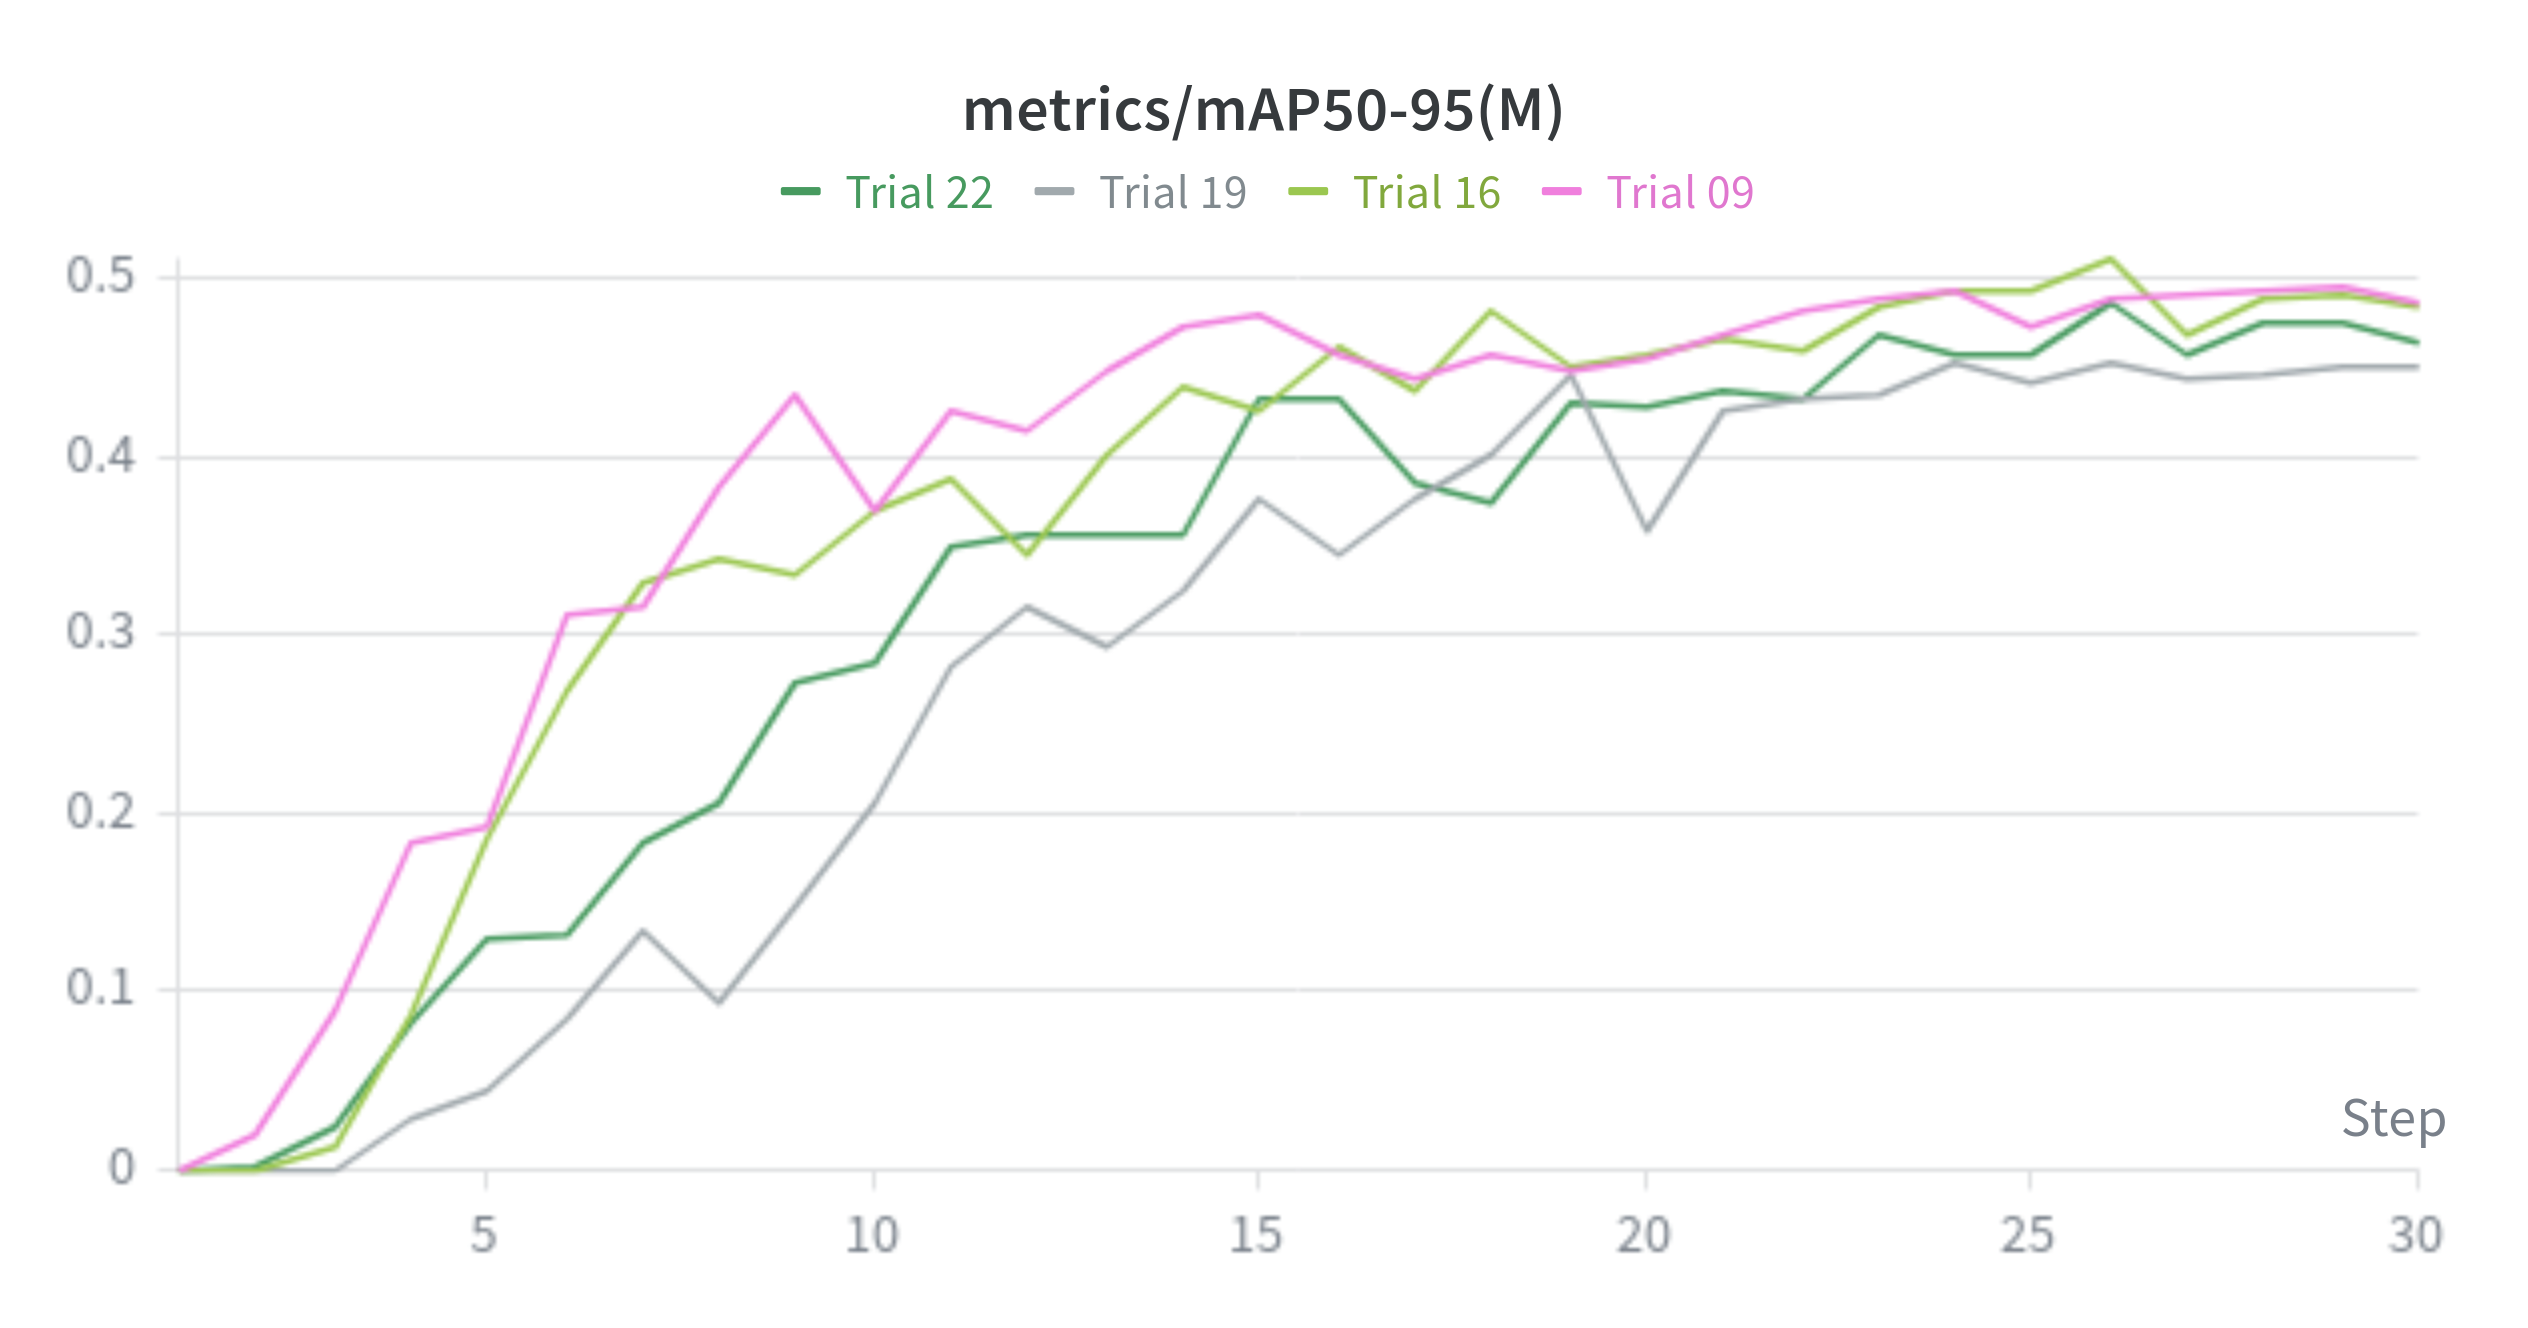
\includegraphics[width=0.82\textwidth]{figures/results/stage1_yolo_trials_mAP50-95_M.png}
    \caption{Validation mask $\mathrm{mAP}_{50\text{:}95}$ for the successful Stage 1 hyperparameter trials.}
    \label{fig:stage1_mask_map}
\end{figure}

\begin{figure}[H]
    \centering
    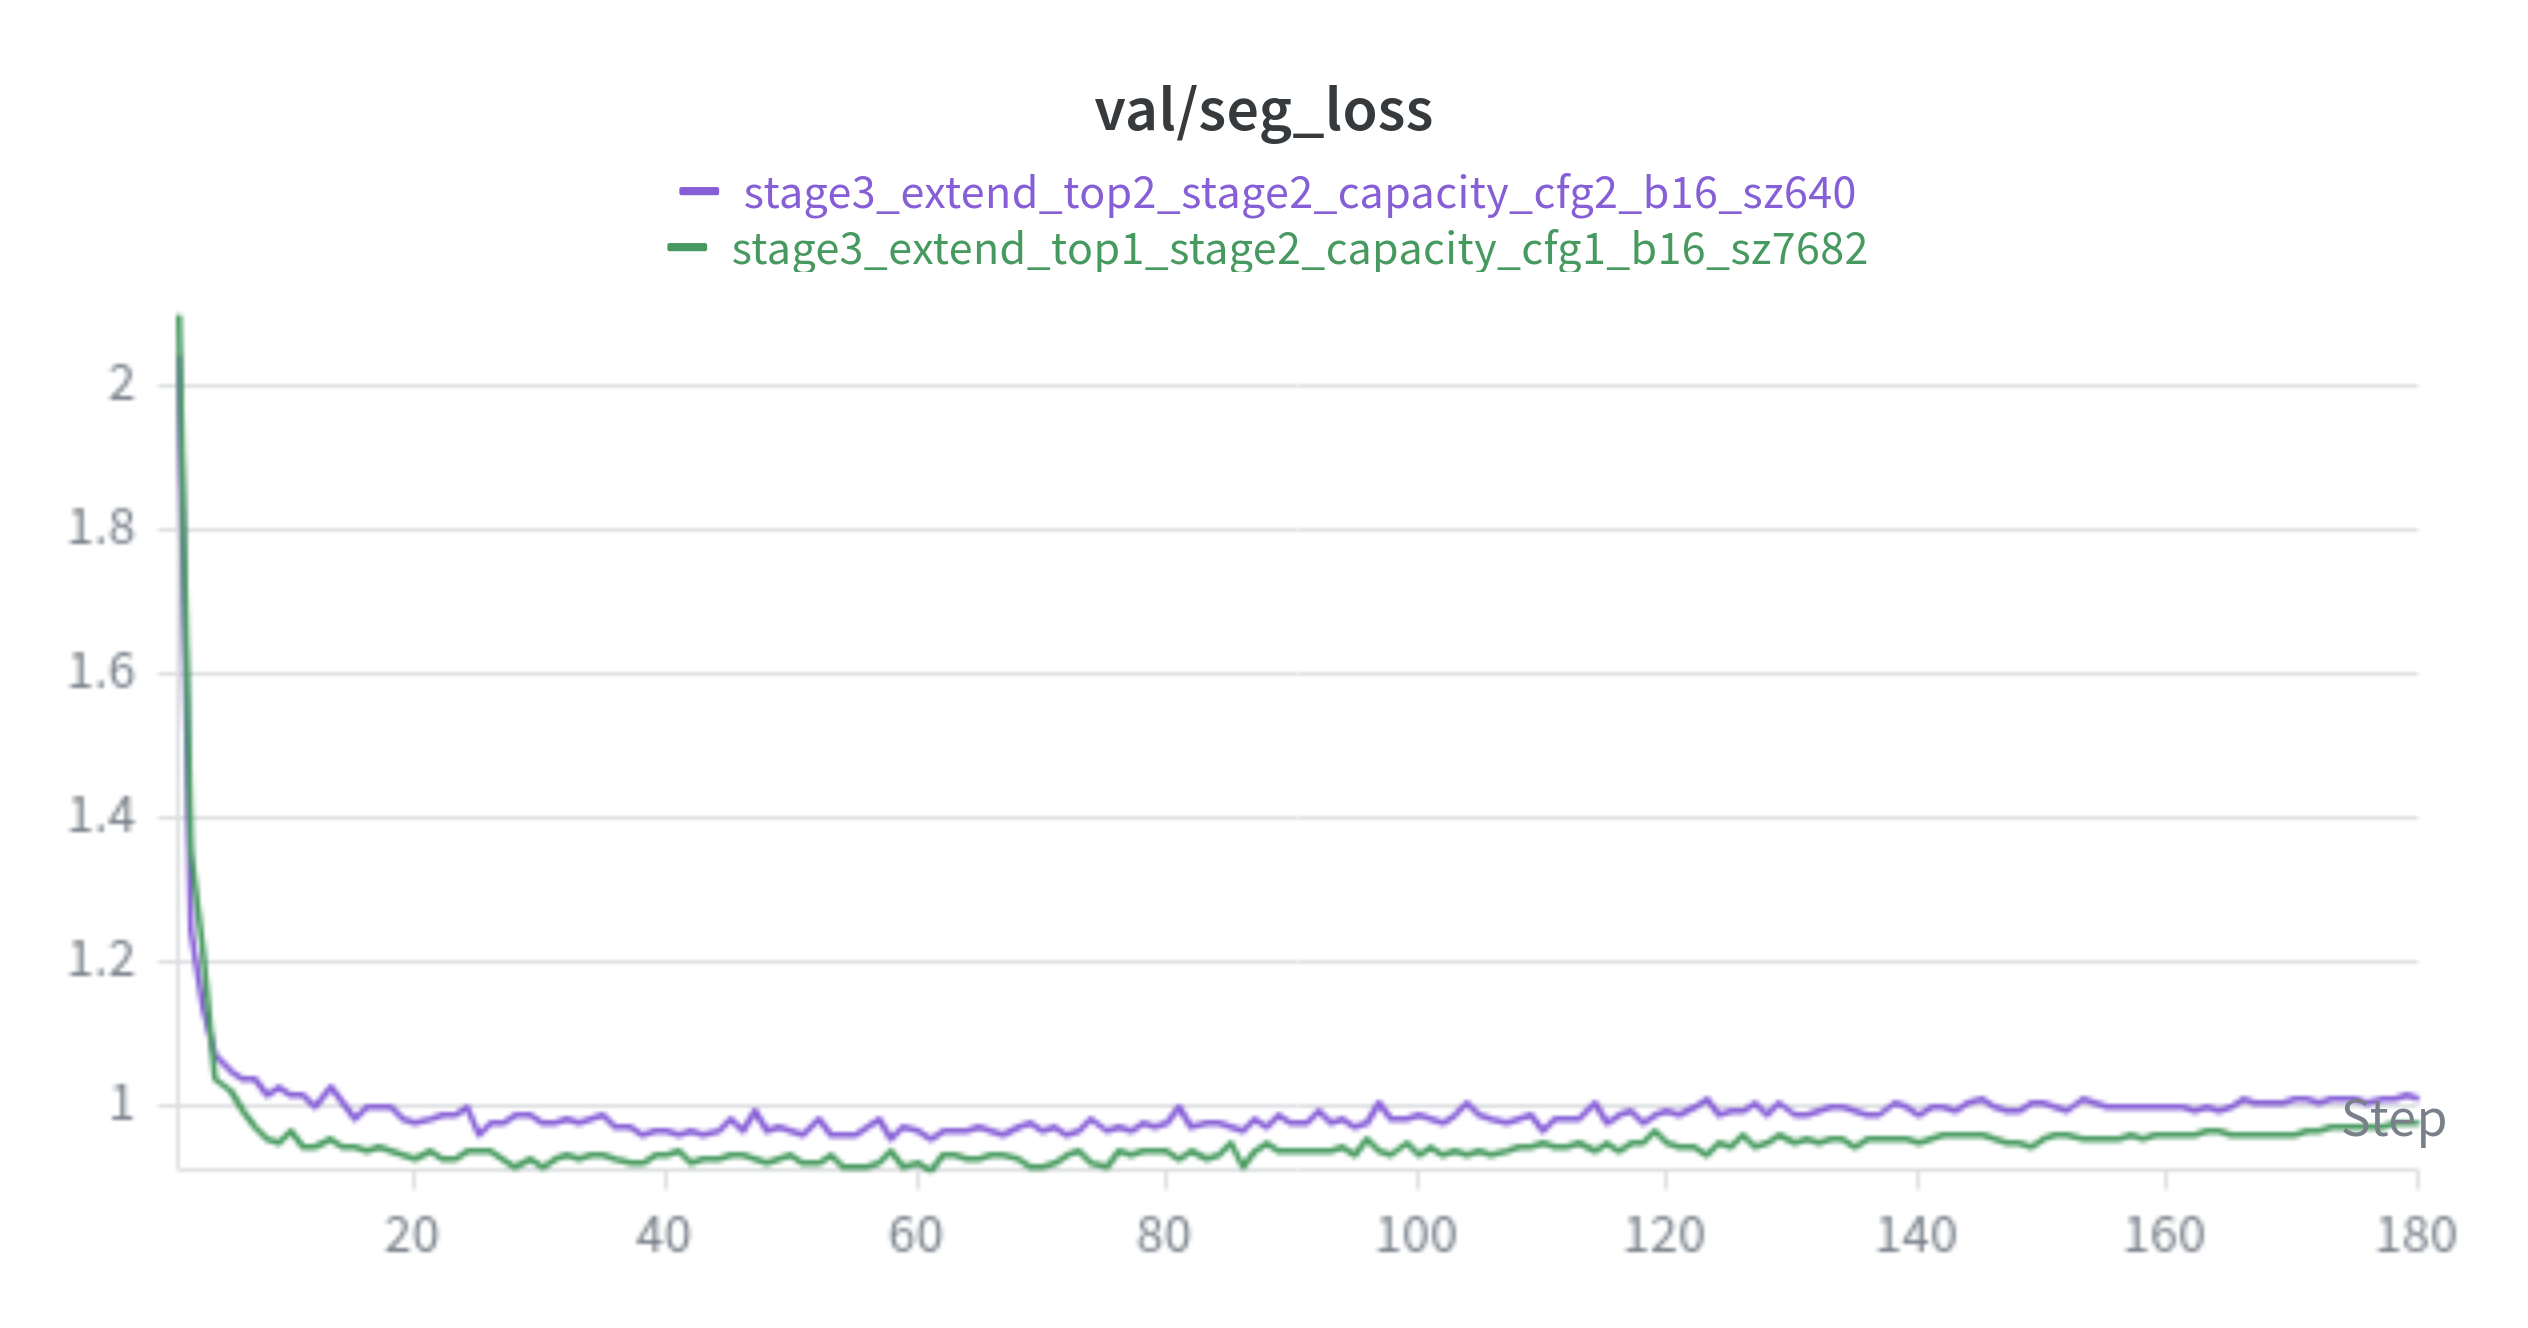
\includegraphics[width=0.82\textwidth]{figures/results/stage3_yolo_val_seg_loss.png}
    \caption{Stage 3 validation segmentation loss for the two refinement branches.}
    \label{fig:stage3_val_seg_loss}
\end{figure}

\begin{figure}[H]
    \centering
    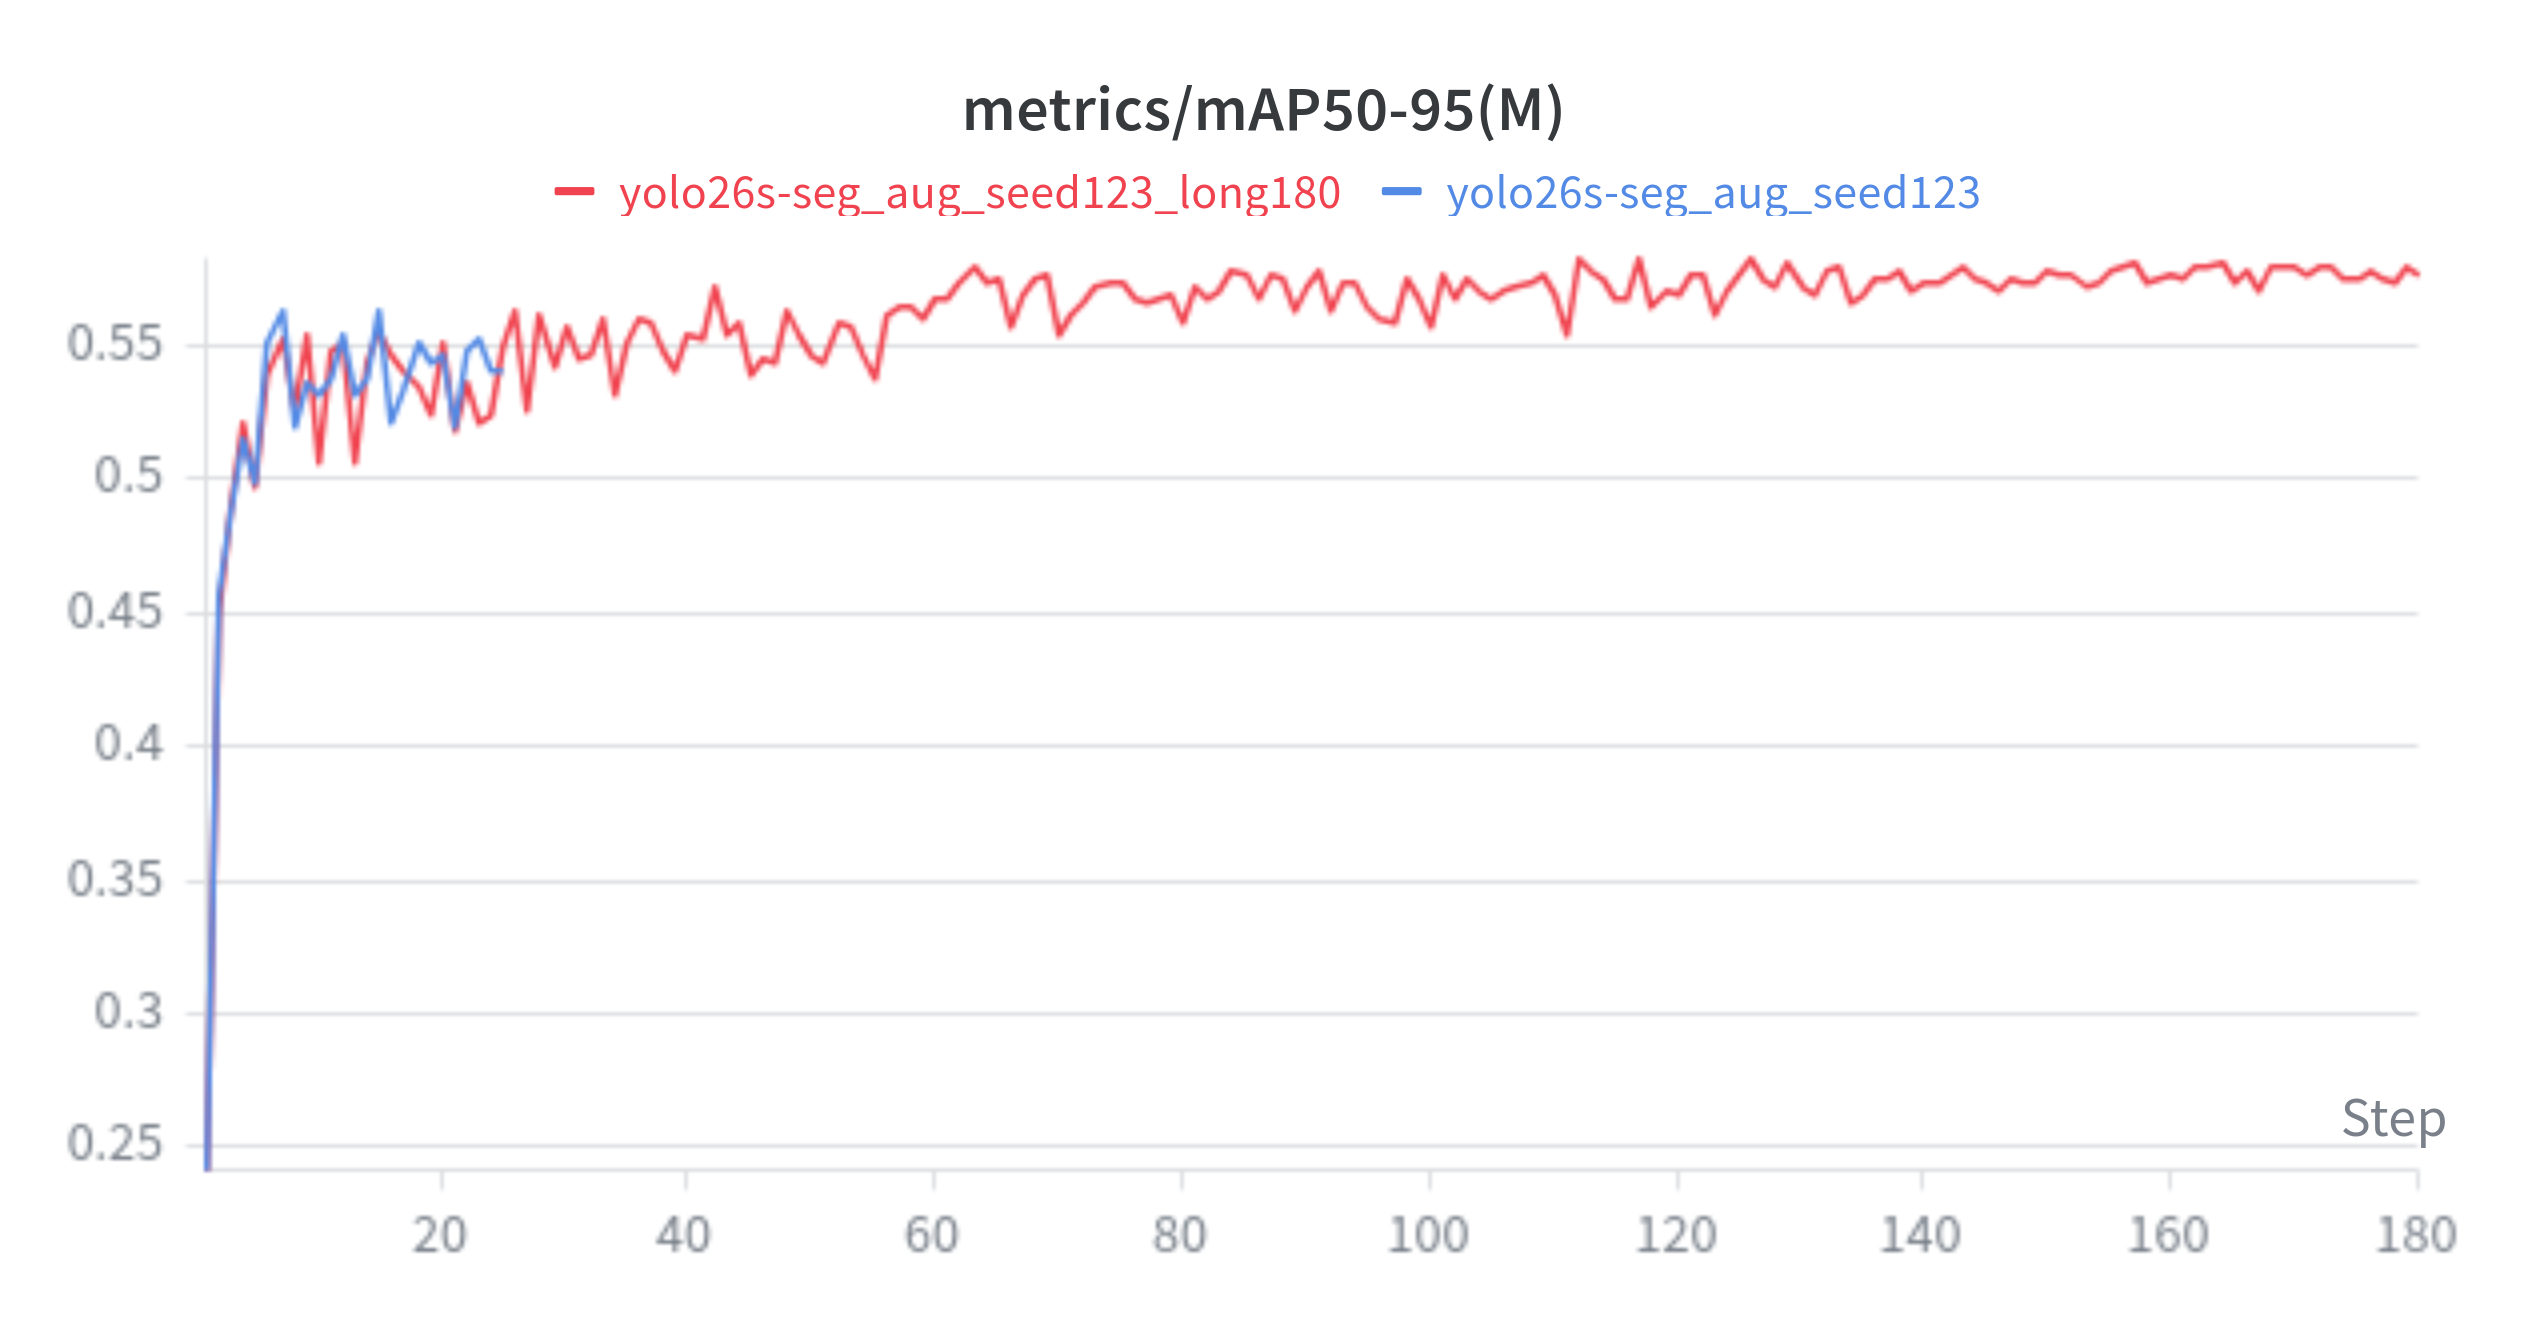
\includegraphics[width=0.82\textwidth]{figures/results/yolo26_mAP50-95_M.png}
    \caption{Validation mask $\mathrm{mAP}_{50\text{:}95}$ for the two YOLO26 training runs.}
    \label{fig:yolo26_mask_map}
\end{figure}

\section{OCR hyperparameter tuning curves}
\label{app:ocr_hparam_curves}

This appendix collects supporting \gls{ocr} hyperparameter-tuning curves that
complement the main validation-accuracy figure and the stage-summary tables in
Chapter~\ref{ch:results}.

\begin{figure}[H]
    \centering
    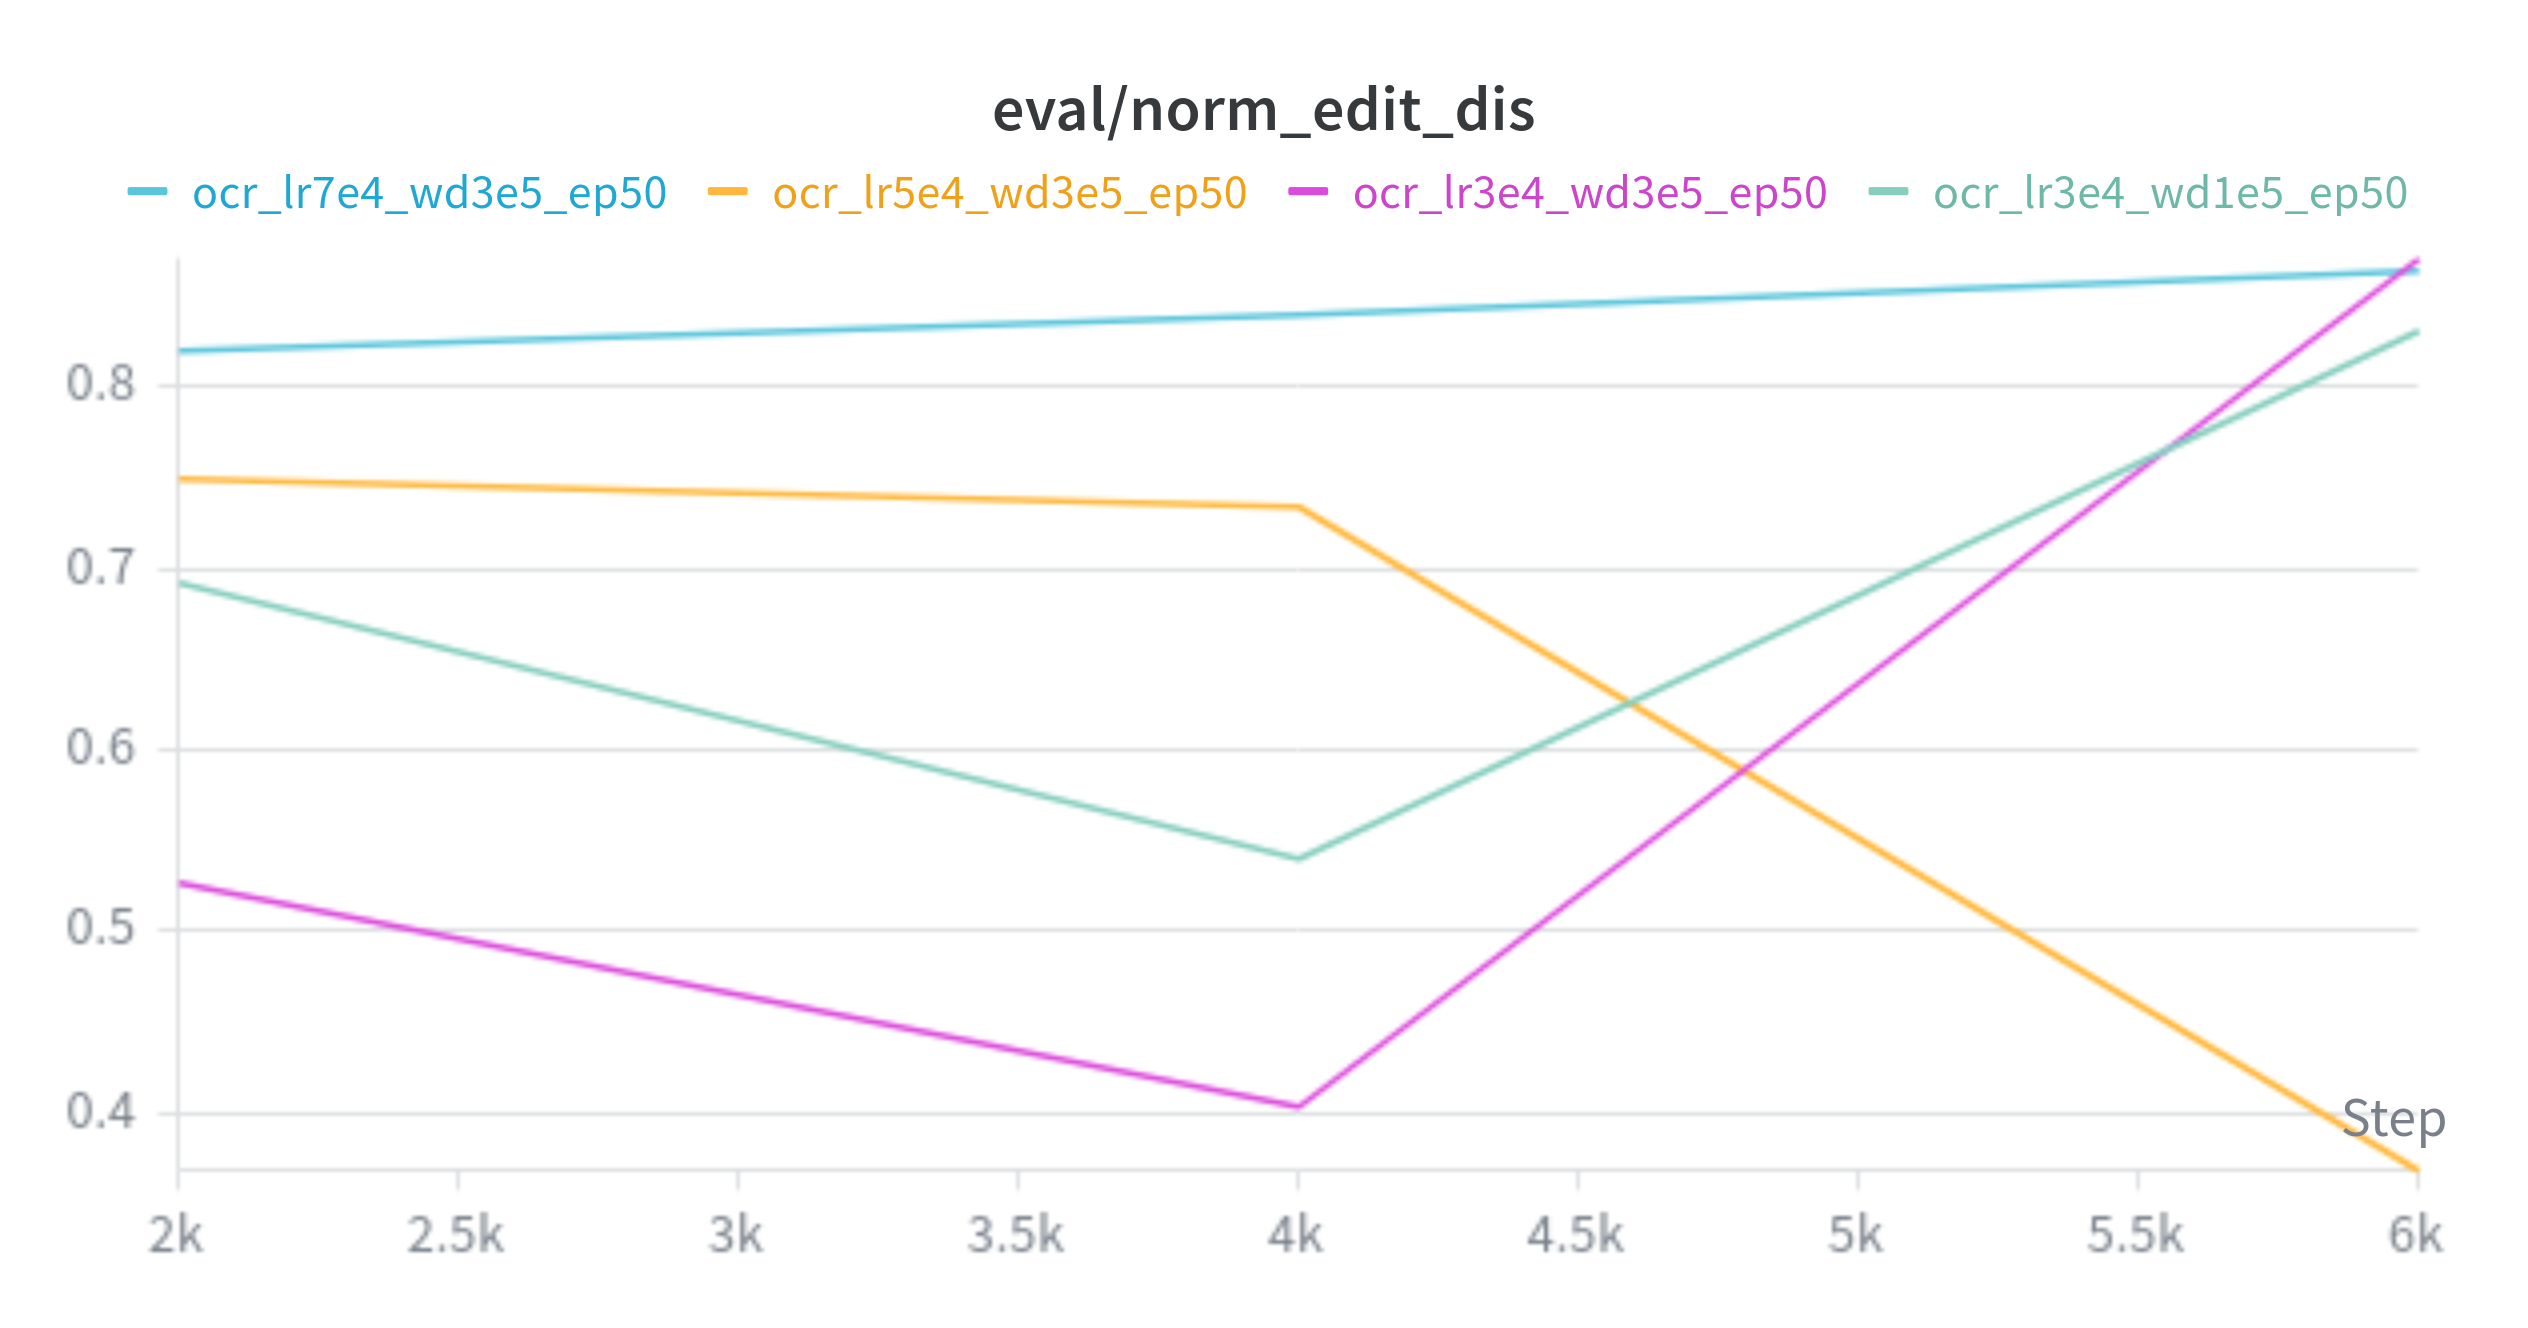
\includegraphics[width=0.82\textwidth]{figures/results/stage2_ocr_eval_norm_edit_dis.png}
    \caption{Stage 2 \gls{ocr} normalized edit distance for the learning-rate and weight-decay sweep.}
    \label{fig:ocr_stage2_ned}
\end{figure}

\clearpage

\chapter{Supplementary model evaluations}
\label{app:maskrcnn_checkpoints}

\section{Mask R-CNN checkpoint progression during annotation support}

The \gls{maskrcnn} model was used as an annotation-support model within the
\gls{cvat}--Nuclio workflow, rather than as the final deployment model. During
dataset construction, the model was retrained several times as more annotated
images became available. To quantify the effect of this iterative retraining, four
checkpoints were evaluated on the same held-out test split used for the
annotation dataset. Table~\ref{tab:maskrcnn_checkpoint_progression} reports both
bounding-box and mask metrics, with mask \gls{ap} treated as the primary
segmentation indicator.

\begin{table}[htbp]
    \centering
    \caption{Held-out test-set performance of the annotation-support \gls{maskrcnn}
    checkpoints as the training set grew during the annotation process.}
    \label{tab:maskrcnn_checkpoint_progression}
    \begin{tabular}{lcccc}
        \toprule
        Checkpoint stage & Training images & BBox AP@[.50:.95] & Mask AP@[.50:.95] & Mask AP@0.50 \\
        \midrule
        Initial checkpoint & 90 & 0.5878 & 0.5844 & 0.7776 \\
        Retrained checkpoint & 449 & 0.6682 & 0.6660 & 0.8284 \\
        Retrained checkpoint & 900 & 0.7007 & 0.6903 & 0.8772 \\
        Final checkpoint & 1400 & 0.7192 & 0.7000 & 0.8990 \\
        \bottomrule
    \end{tabular}
\end{table}

The results show a consistent improvement trend as the amount of annotated data
increased. The largest gain was observed between the initial 90-image checkpoint
and the first larger retrained checkpoint at 449 images, while later retraining
to 900 and 1400 images provided smaller but still measurable improvements. On
the primary mask metric, AP@[0.50:0.95] increased from 0.5844 to 0.7000. This
supports the annotation strategy adopted in this project: iterative retraining of
the pre-annotation model improved the quality of automatically proposed
instances, thereby reducing the manual correction burden in later annotation
rounds.

\chapter{Supplementary deployment experiments}
\label{app:adc_replay_appendix}

This appendix collects supplementary deployment-oriented analyses that support the
main-body results of Section~\ref{sec:adc_finetuning_results} and
Section~\ref{sec:ros_pipeline_results}. The main chapter presents the most
compact figures under page constraints, while the appendix retains additional
deployment behavior that was informative during interpretation.

\section{Unfiltered single-button detector comparison}

Table~\ref{tab:appendix_unfiltered_single_button} shows the same controlled R29
single-button experiment before the baseline-model detections above 1.5~m were
removed. It is included to document the full deployment behavior of both models.
The apparent long-range advantage of the baseline model in the unfiltered distance
statistics should not be interpreted as better valid detection range, because manual
review showed that all twelve baseline detections above 1.5~m were false positives.

\begin{table}[htbp]
    \centering
    \caption{Unfiltered controlled single-button comparison on the same recorded \gls{ros} bag from HAN Building R29.}
    \label{tab:appendix_unfiltered_single_button}
    \small
    \begin{tabular}{lcc}
        \toprule
        Metric & Baseline model & \glsentryshort{adc} fine-tuned model \\
        \midrule
        Frames with detected buttons & 116 & 138 \\
        Mean target confidence & 0.7855 & 0.8069 \\
        Median target confidence & 0.8328 & 0.8423 \\
        Mean valid-target distance [m] & 0.4408 & 0.4282 \\
        Median valid-target distance [m] & 0.3353 & 0.4102 \\
        Maximum valid-target distance [m] & 1.6536 & 0.8761 \\
        \bottomrule
    \end{tabular}
\end{table}

\section{Single-button end-to-end confidence behavior}

Besides the detector-only baseline-versus-\glsentryshort{adc} comparison shown in the main
body, the controlled single-button R29 replay was also inspected at the full
\gls{yolo}+\gls{ocr} pipeline level. Figure~\ref{fig:appendix_single_button_yolo_ocr_confidence}
shows the detector confidence together with the downstream \gls{ocr} confidence
for the same run. Correct \texttt{UP} reads remain clustered in the lower-to-mid
distance range, while the few \gls{ocr} errors appear at larger distances within
that run.

\begin{figure}[htbp]
    \centering
    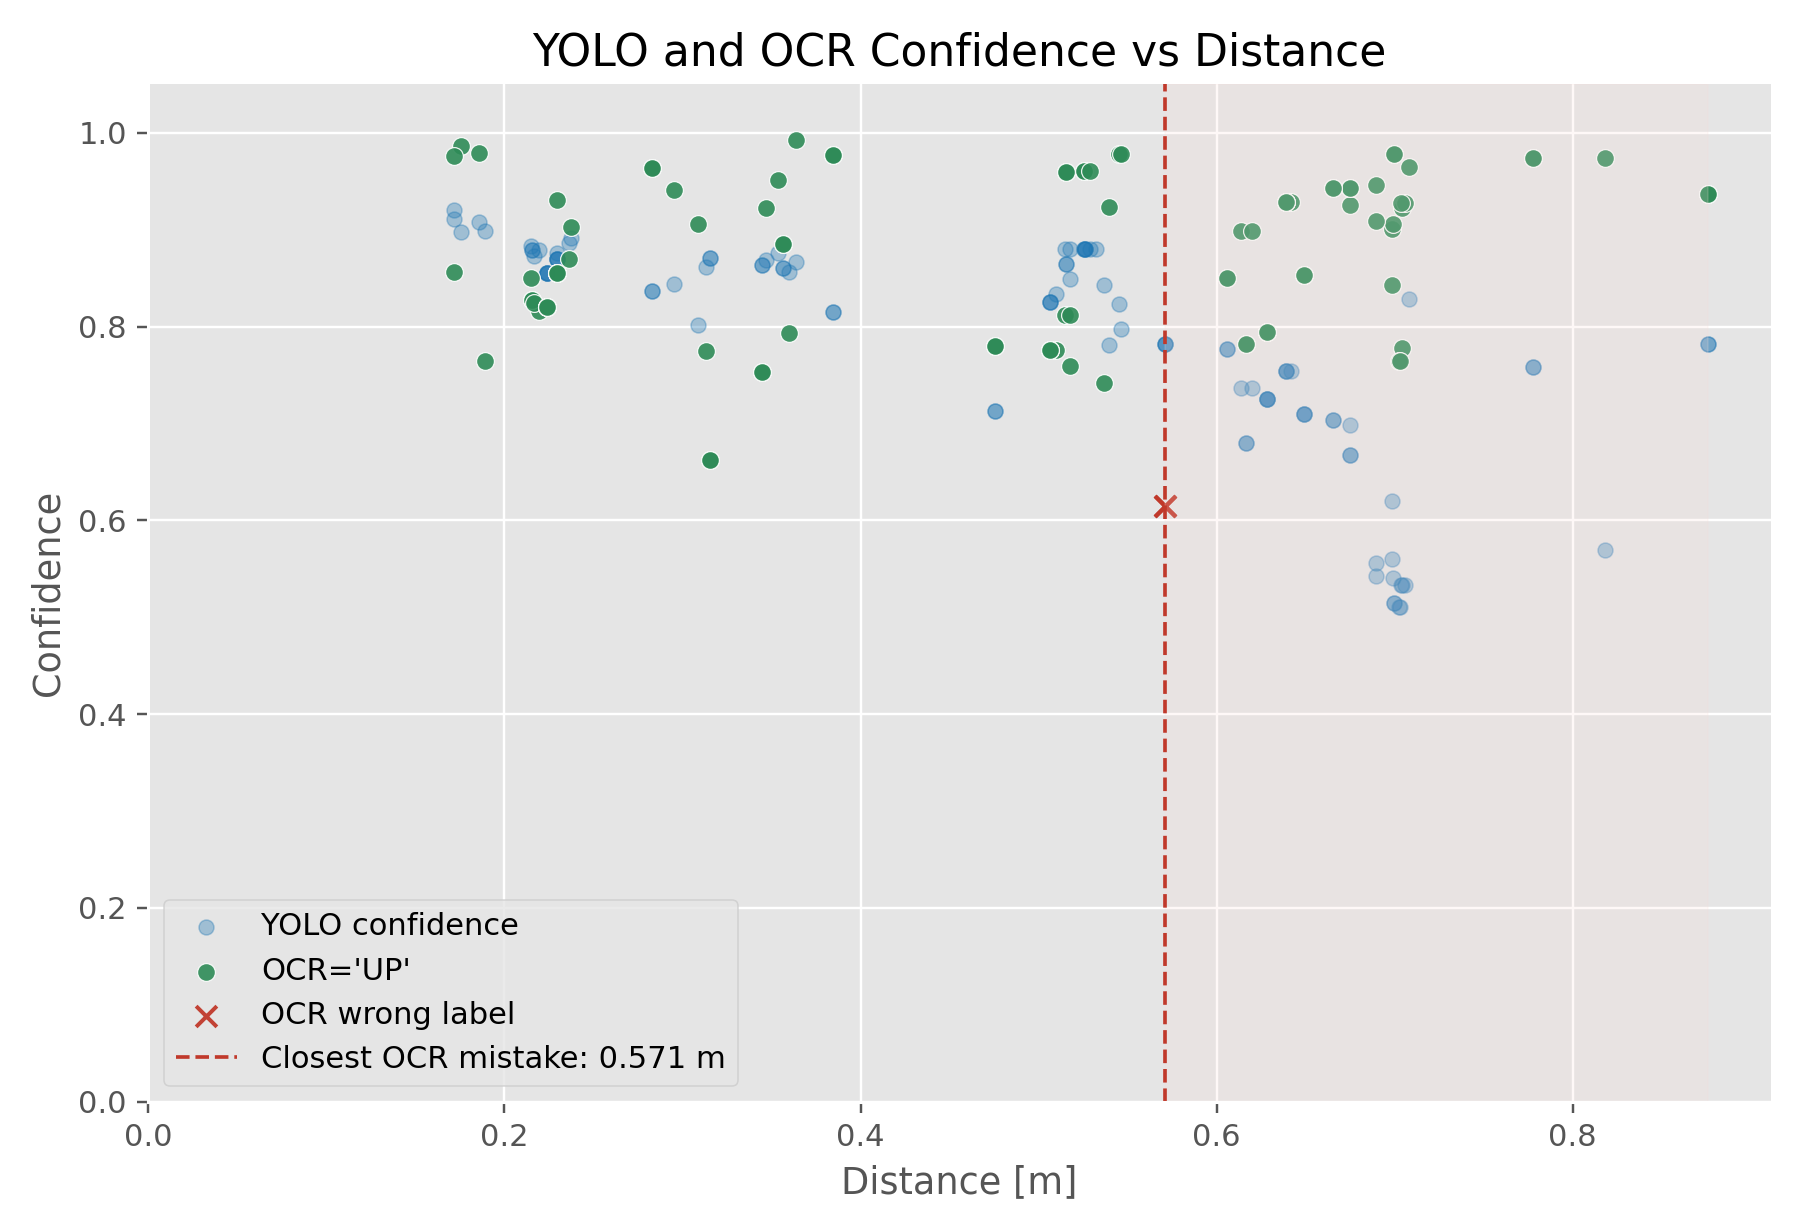
\includegraphics[width=0.82\textwidth]{figures/appendices/single_button_yolo_ocr_confidence_distance.png}
    \caption{Supplementary single-button R29 replay plot showing \gls{yolo} confidence, \gls{ocr} confidence, and the distances at which \gls{ocr} stopped reading the \texttt{UP} button correctly.}
    \label{fig:appendix_single_button_yolo_ocr_confidence}
\end{figure}

\section{Mixed-environment replay review by distance bin}

A second replay analysis was performed on a longer university elevator bag that
contained multiple panels, cluttered backgrounds, and changing viewpoints. The
detections were manually reviewed as true positives or false positives after
replay. Figure~\ref{fig:appendix_reviewed_tp_fp_distance_bins} shows the reviewed
true- and false-positive counts by distance bin for that broader run. The figure
is included as supporting evidence for the realistic deployment trend discussed
in Section~\ref{sec:ros_pipeline_results}: reviewed detections were highly
reliable below roughly 1.5~m, whereas the longer-range bins were dominated by
false positives.

\begin{figure}[htbp]
    \centering
    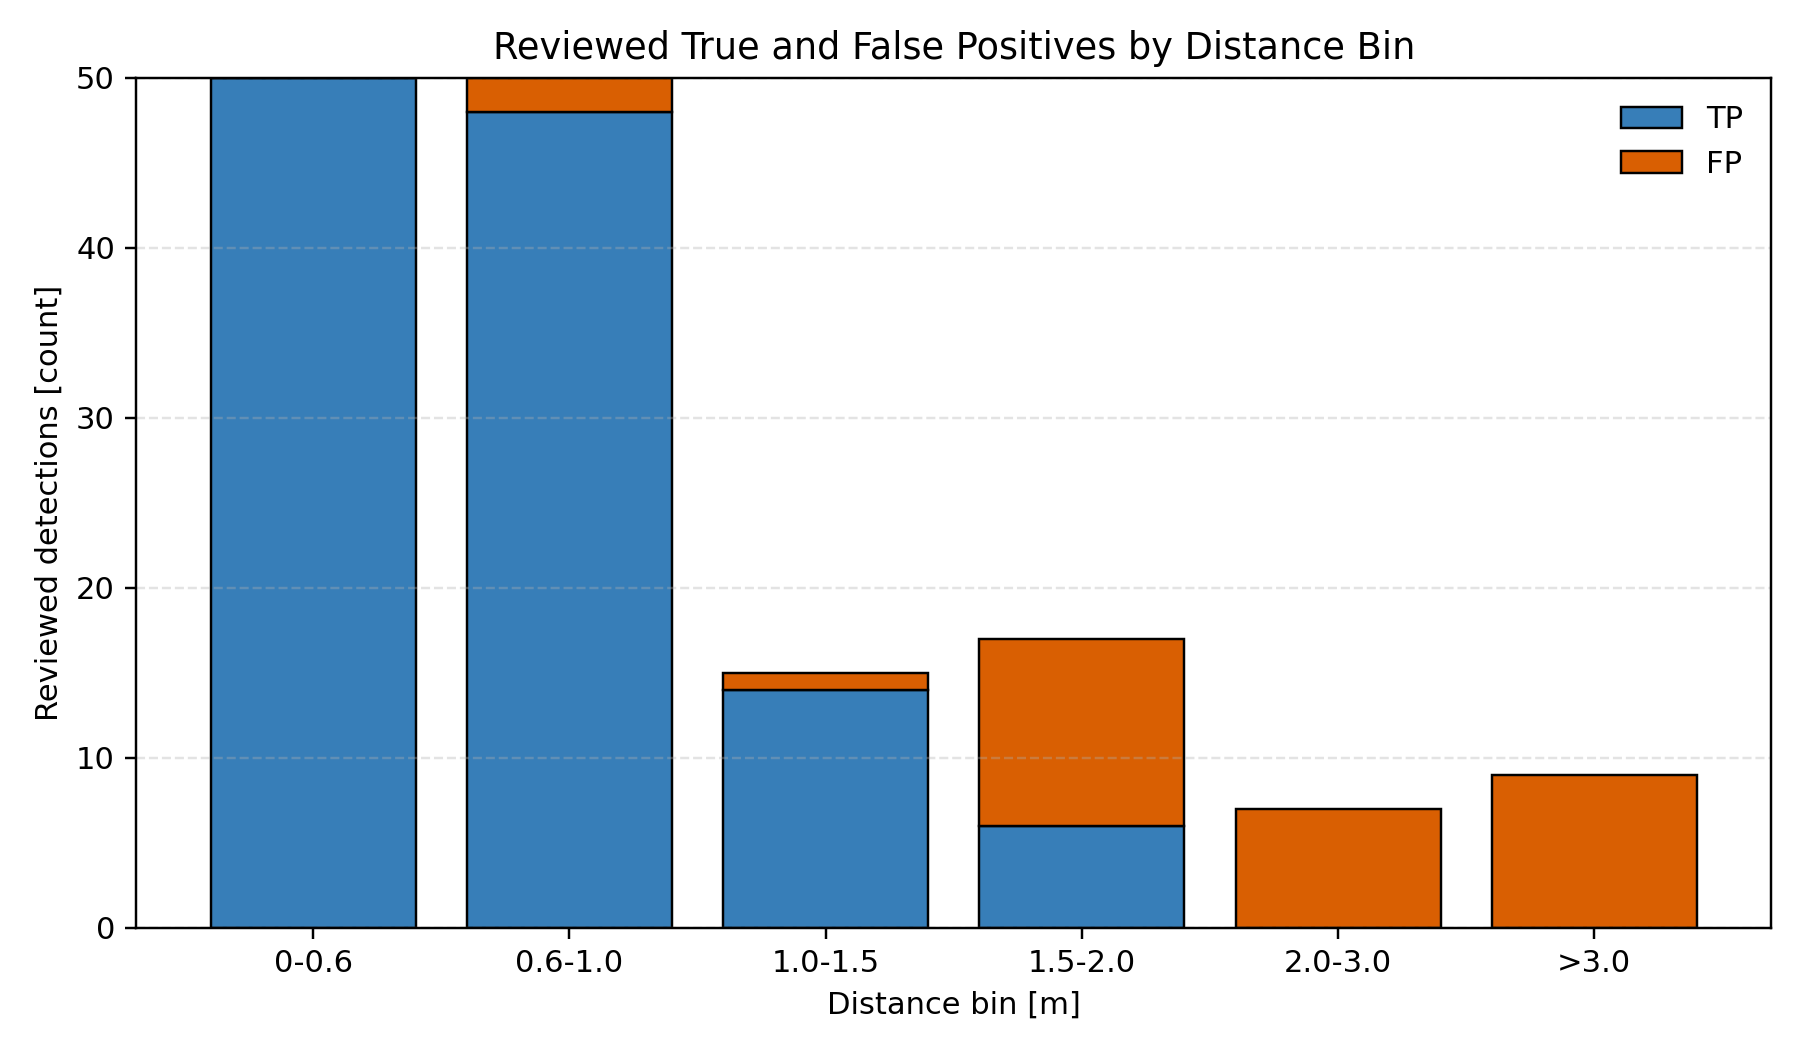
\includegraphics[width=0.82\textwidth]{figures/appendices/reviewed_tp_fp_by_distance_bin.png}
    \caption{Reviewed true and false positive detections by distance bin on the longer university replay run. Close-range bins were sampled, while the longer-distance bins were reviewed exhaustively.}
    \label{fig:appendix_reviewed_tp_fp_distance_bins}
\end{figure}

\chapter{Supplementary dataset quality plots}
\label{app:dataset_quality_plots}

This appendix provides compact visual support for the dataset quality
assessment summarized in Chapter~4. The figures are included only as supporting
material and are not required to follow the main argument of the report.

\section{Image-level quality distributions}

\begin{figure}[htbp]
    \centering
    
\includegraphics[width=0.82\textwidth]
    {../../master_thesis_carebot_2025/annotations_zips/dataset_quality_analysis/quality_plots/01_blur_distribution.png}
    \caption{Distribution of the blur indicator computed from the training
    images. The spread confirms that the dataset contains both softer and
    sharper images instead of a single tightly controlled acquisition setting.}
    \label{fig:app_blur_distribution}
\end{figure}

\begin{figure}[htbp]
    \centering
    
\includegraphics[width=0.82\textwidth]
    {../../master_thesis_carebot_2025/annotations_zips/dataset_quality_analysis/quality_plots/05_brightness_distribution.png}
    \caption{Distribution of the mean grayscale intensity across the training
    images. The dataset spans a broad but still usable range of illumination
    conditions.}
    \label{fig:app_brightness_distribution}
\end{figure}

\section{Spatial button distribution}

\begin{figure}[htbp]
    \centering
    
\includegraphics[width=0.82\textwidth]
    {../../master_thesis_carebot_2025/annotations_zips/dataset_quality_analysis/geometry_plots/B_button_centroid_heatmap.png}
    \caption{Heatmap of annotated button-centroid locations in normalized image
    coordinates. Most button instances lie within a central field-of-view band,
    while edge-of-frame occurrences are less frequent.}
    \label{fig:app_button_centroid_heatmap}
\end{figure}

\chapter{\Gls{ros2} pipeline parameter reference}
\label{app:ros2_params}

This appendix summarizes the main runtime parameters of the deployed
\gls{ros2} perception pipeline. The tables are intended as a practical reference
for reproducing experiments or adjusting node behavior during deployment. Values
shown in the ``Default / configured value'' column correspond to the final thesis
configuration where this was defined explicitly in the YAML files; otherwise the
node's declared software default is reported.

\section{YOLO inference node}

\small
\begin{longtable}{p{4.2cm} p{3.2cm} p{7.3cm}}
\caption{Main parameters of \texttt{yolo\_engine\_node}.}
\label{tab:app_yolo_params}\\
\toprule
\textbf{Parameter} & \textbf{Default / configured value} & \textbf{Purpose} \\
\midrule
\endfirsthead
\toprule
\textbf{Parameter} & \textbf{Default / configured value} & \textbf{Purpose} \\
\midrule
\endhead
\texttt{engine\_path} & launch-time path & Path to the \gls{tensorrt} \gls{yolo} engine. \\
\texttt{image\_topic} & \texttt{/zed/zed\_node/rgb/color/rect/image} & Input image topic. \\
\texttt{depth\_topic} & \texttt{/zed/zed\_node/depth/depth\_registered} & Input depth topic used for 3D projection. \\
\texttt{camera\_info\_topic} & \texttt{/zed/zed\_node/rgb/color/rect/camera\_info} & Camera intrinsics topic. \\
\texttt{detections\_topic} & \texttt{/detections} & Optional 2D detection topic retained for debugging. \\
\texttt{targets\_3d\_topic} & \texttt{/button\_targets\_3d} & Main 3D target output topic. \\
\texttt{conf} & 0.50 & Confidence threshold for accepted detections. \\
\texttt{infer\_hz} & 8.0 & Timer frequency for inference callbacks. \\
\texttt{enable\_distance\_estimation} & \texttt{true} & Enables depth-based 3D target estimation. \\
\texttt{max\_depth\_age\_ms} & 150.0 & Maximum allowed age of buffered depth data. \\
\texttt{min\_depth\_m} & 0.10 & Minimum accepted depth value. \\
\texttt{max\_depth\_m} & 10.0 & Maximum accepted depth value. \\
\texttt{min\_valid\_depth\_pixels} & 20 & Minimum number of valid masked depth pixels. \\
\texttt{depth\_percentile} & 50.0 & Percentile used for representative target depth. \\
\texttt{enable\_ocr} & \texttt{false} & Legacy inline \gls{ocr} mode; disabled in the split-node pipeline. \\
\texttt{ocr\_engine\_path} & empty & Optional legacy inline \gls{ocr} engine path. \\
\texttt{ocr\_input\_name} & \texttt{x} & Legacy inline \gls{ocr} input tensor name. \\
\texttt{ocr\_charset\_path} & empty & Optional legacy inline \gls{ocr} character set path. \\
\texttt{ocr\_input\_h} & 48 & Legacy inline \gls{ocr} input height. \\
\texttt{ocr\_input\_w} & 320 & Legacy inline \gls{ocr} input width. \\
\texttt{ocr\_min\_conf} & 0.60 & Legacy inline \gls{ocr} confidence threshold. \\
\texttt{ocr\_max\_rois\_per\_frame} & 8 & Legacy inline \gls{ocr} ROI cap. \\
\texttt{warmup\_runs} & 3 & Number of startup warmup inferences. \\
\texttt{enable\_mask\_rle\_export} & \texttt{false} & Enables direct mask export for dataset collection. \\
\texttt{publish\_debug\_image} & \texttt{true} & Enables publication of a visual debug image. \\
\texttt{debug\_image\_topic} & \texttt{/yolo/debug\_image} & Debug image output topic. \\
\texttt{enable\_perf\_logging} & \texttt{true} & Enables periodic runtime timing logs. \\
\texttt{perf\_log\_every\_n} & 50 & Logging interval for performance statistics. \\
\bottomrule
\end{longtable}
\normalsize

\section{\Gls{ocr} inference node}

\small
\begin{longtable}{p{4.2cm} p{3.2cm} p{7.3cm}}
\caption{Main parameters of \texttt{ocr\_trt\_node}.}
\label{tab:app_ocr_params}\\
\toprule
\textbf{Parameter} & \textbf{Default / configured value} & \textbf{Purpose} \\
\midrule
\endfirsthead
\toprule
\textbf{Parameter} & \textbf{Default / configured value} & \textbf{Purpose} \\
\midrule
\endhead
\texttt{image\_topic} & \texttt{/zed/zed\_node/rgb/color/rect/image} & Input image topic used for buffered crops. \\
\texttt{targets\_topic\_in} & \texttt{/button\_targets\_3d} & Input topic from the \gls{yolo} node. \\
\texttt{targets\_topic\_out} & \texttt{/button\_targets\_3d\_ocr} & Output topic with text-enriched targets. \\
\texttt{debug\_image\_topic} & \texttt{/ocr/debug\_image} & Debug visualization topic. \\
\texttt{ocr\_engine\_path} & launch-time path & Path to the \gls{tensorrt} \gls{ocr} engine. \\
\texttt{ocr\_input\_name} & \texttt{x} & Name of the input tensor in the engine. \\
\texttt{ocr\_charset\_path} & empty & Optional character set file path. \\
\texttt{ocr\_input\_h} & 48 & Input crop height for recognition. \\
\texttt{ocr\_input\_w} & 320 & Input crop width for recognition. \\
\texttt{ocr\_min\_conf} & 0.60 & Minimum accepted text confidence. \\
\texttt{ocr\_max\_rois\_per\_msg} & 8 & Maximum number of button crops processed per message. \\
\texttt{warmup\_runs} & 3 & Number of startup warmup inferences. \\
\texttt{max\_image\_age\_ms} & 220.0 & Maximum age of buffered image data matched to a target message. \\
\texttt{image\_buffer\_size} & 30 & Number of recent images retained for matching. \\
\texttt{publish\_debug\_image} & declared default \texttt{true} & Enables publication of the \gls{ocr} debug image. \\
\texttt{enable\_perf\_logging} & declared default \texttt{true} & Enables periodic timing logs. \\
\texttt{perf\_log\_every\_n} & declared default 50 & Logging interval for performance statistics. \\
\texttt{enable\_fuzzy\_map} & \texttt{true} & Enables post-recognition vocabulary correction. \\
\texttt{label\_vocab\_path} & configured file path & Path to known elevator button labels. \\
\texttt{fuzzy\_max\_dist} & 1 & Maximum edit distance for fuzzy label correction. \\
\texttt{fuzzy\_min\_len} & 3 & Minimum string length before fuzzy matching is applied. \\
\texttt{fuzzy\_min\_score} & 0.0 & Minimum score required before fuzzy correction is considered. \\
\bottomrule
\end{longtable}
\normalsize

\section{\Gls{adc}}

\small
\begin{longtable}{p{4.2cm} p{3.2cm} p{7.3cm}}
\caption{Main parameters of \texttt{active\_data\_collector}.}
\label{tab:app_adc_params}\\
\toprule
\textbf{Parameter} & \textbf{Default / configured value} & \textbf{Purpose} \\
\midrule
\endfirsthead
\toprule
\textbf{Parameter} & \textbf{Default / configured value} & \textbf{Purpose} \\
\midrule
\endhead
\texttt{image\_topic} & \texttt{/zed/zed\_node/rgb/color/rect/image} & Input image topic. \\
\texttt{targets\_topic} & \texttt{/button\_targets\_3d\_ocr} & Input target topic from the \gls{ocr} node. \\
\texttt{dataset\_root} & configured dataset path & Root folder for collected sessions. \\
\texttt{session\_name} & empty & Optional explicit session name. \\
\texttt{save\_overlay\_image} & \texttt{true} & Saves an annotated overlay image for each accepted sample. \\
\texttt{overlay\_font\_scale} & 0.30 & Font size used in overlay rendering. \\
\texttt{overlay\_font\_thickness} & 1 & Font thickness used in overlay rendering. \\
\texttt{max\_image\_age\_ms} & 250.0 & Maximum age of the buffered image matched to a target message. \\
\texttt{image\_buffer\_size} & 40 & Number of recent images retained for timestamp matching. \\
\texttt{enable\_perf\_logging} & declared default \texttt{true} & Enables periodic collector timing logs. \\
\texttt{perf\_log\_every\_n} & declared default 20 & Logging interval for collector performance statistics. \\
\texttt{min\_targets\_per\_frame} & 1 & Minimum number of accepted targets required for export. \\
\texttt{min\_target\_score} & 0.45 & Minimum detector score for a target candidate. \\
\texttt{require\_text} & \texttt{True} & Requires accepted \gls{ocr} output before export. \\
\texttt{min\_text\_score} & 0.45 & Minimum accepted \gls{ocr} confidence. \\
\texttt{min\_export\_interval\_sec} & 0.75 & Minimum time gap between accepted exports. \\
\texttt{min\_bbox\_area\_pixels} & 100.0 & Minimum target bounding-box area. \\
\texttt{min\_bbox\_short\_side\_pixels} & 10.0 & Minimum short side of the target box. \\
\texttt{min\_image\_brightness} & 35.0 & Lower image brightness gate. \\
\texttt{max\_image\_brightness} & 235.0 & Upper image brightness gate. \\
\texttt{max\_saturated\_ratio} & 0.25 & Maximum saturated-pixel ratio. \\
\texttt{enable\_sharpness\_gate} & \texttt{true} & Enables whole-image sharpness filtering. \\
\texttt{min\_laplacian\_var} & 120.0 & Minimum whole-image Laplacian variance. \\
\texttt{enable\_roi\_sharpness\_gate} & \texttt{true} & Enables target-ROI sharpness filtering. \\
\texttt{min\_roi\_laplacian\_var} & 40.0 & Minimum ROI Laplacian variance. \\
\texttt{enable\_stability\_gate} & \texttt{true} & Enables temporal stability filtering across frames. \\
\texttt{stability\_required\_frames} & 3 & Number of supporting frames required for export. \\
\texttt{stability\_iou\_threshold} & 0.40 & IoU threshold for matching targets across frames. \\
\texttt{stability\_depth\_tolerance\_m} & 0.20 & Depth consistency threshold in meters. \\
\texttt{stability\_track\_ttl\_sec} & 1.2 & Lifetime of a temporary stability track. \\
\texttt{stability\_require\_ocr\_consistency} & \texttt{true} & Requires stable \gls{ocr} content across the track. \\
\texttt{enable\_dedup} & \texttt{true} & Enables duplicate-frame rejection. \\
\texttt{dedup\_hamming\_threshold} & 8 & Hamming threshold for duplicate detection. \\
\texttt{dedup\_history\_size} & 50 & Number of recent accepted samples used for deduplication. \\
\texttt{analysis\_ocr\_score\_threshold} & 0.60 & Threshold used for analysis-only \gls{ocr} statistics. \\
\texttt{distance\_bin\_size\_m} & 0.25 & Bin size for distance-distribution statistics. \\
\texttt{max\_analysis\_distance\_m} & 5.0 & Maximum distance included in exported analysis summaries. \\
\bottomrule
\end{longtable}
\normalsize


\end{document}
